%--------------------------------------------------------------------%
%
% Berkas utama templat LaTeX.
%
% author Petra Barus, Peb Ruswono Aryan, Faris Rizki Ekananda
%
%--------------------------------------------------------------------%
%
% Berkas ini berisi struktur utama dokumen LaTeX yang akan dibuat.
%
%--------------------------------------------------------------------%

\documentclass[bahasa, 12pt, a4paper, onecolumn, oneside, final]{report}

%-------------------------------------------------------------------%
%
% Konfigurasi dokumen LaTeX untuk laporan tesis IF ITB
%
% @author Petra Novandi
%
%-------------------------------------------------------------------%
%
% Berkas asli berasal dari Steven Lolong
%
%-------------------------------------------------------------------%

% Ukuran kertas
\special{papersize=210mm,297mm}

% Setting margin
\usepackage[top=2cm,bottom=2cm,left=4cm,right=3cm]{geometry}

% remove hyphenation
% \hbadness=99999

% % Disable hyphenation
% \hyphenpenalty=10000
% \exhyphenpenalty=10000
% \tolerance=1000

% Math package
\usepackage{mathptmx}

% 4th Sectioning
\usepackage{titlesec}
\newcommand{\subsubsubsection}[1]{\paragraph{#1}\mbox{}\\}

\titleformat{\subsubsubsection}
{\normalfont\normalsize\bfseries}{\theparagraph}{1em}{}
\titlespacing*{\subsubsubsection}
{0pt}{3.25ex plus 1ex minus .2ex}{1.5ex plus .2ex}

% Judul bahasa Indonesia
\usepackage[bahasa]{babel}

% Format citation
\usepackage[utf8]{inputenc}
% \usepackage[style=authoryear,backend=biber,sorting=nyt]{biblatex}
% \DeclareLanguageMapping{bahasa-cms}{bahasa-cms}
\usepackage[authordate,backend=biber, language=bahasa]{biblatex-chicago}
\AtEveryBibitem{\clearfield{month}}
\usepackage[format=hang, justification=raggedright]{caption}

% Custom settings for tables
\captionsetup[table]{justification=raggedright, singlelinecheck=false, format=hang} % Left-align and hang for tables

\usepackage{csquotes} % Untuk kutipan
\usepackage{amsmath}
\usepackage{longtable}
\usepackage{graphicx}
\usepackage{subfig}
\usepackage{titling}
\usepackage{booktabs}
\usepackage{tabularx}
\usepackage{multirow}

% Define a new column type 'C' for centered columns in tabularx
\newcolumntype{C}{>{\centering\arraybackslash}X}

\usepackage{blindtext}
\usepackage{sectsty}
\usepackage{chngcntr}
\usepackage{etoolbox}
\usepackage{array}
\usepackage[hidelinks]{hyperref}       % Package untuk link di daftar isi. Ubah jadi \usepackage[hidelinks]{hyperref} apabila ingin menghilangkan kotak merah disekitar link
\usepackage{titlesec}       % Package Format judul
\usepackage{titletoc}       % Package Format judul di toc
\usepackage{tocbibind}      % Package untuk masukkan toc, lot, lof ke Daftar Isi
\usepackage{scrwfile}       % Package untuk membuat Daftar Lampiran dari toc
\usepackage{parskip}
\usepackage{afterpage}
\usepackage{relsize}
\usepackage{xcolor, colortbl}
\usepackage{setspace}
\usepackage{listings}

\graphicspath{{resources/}}   % letak direktori penyimpanan gambar

% Setting daftar lampiran
\newcommand*{\lopname}{DAFTAR LAMPIRAN}
\TOCclone[\lopname]{toc}{atoc}
\addtocontents{atoc}{\protect\value{tocdepth}=-1}
\newcommand\listofappendices{
	\cleardoublepage
	\phantomsection
	\listofatoc
	\addcontentsline{toc}{chapter}{\lopname}
}

\newcommand*\savedtocdepth{}
\AtBeginDocument{%
	\edef\savedtocdepth{\the\value{tocdepth}}%
}

\let\originalappendix\appendix
\renewcommand\appendix{%
	\originalappendix
	\cleardoublepage
	\addtocontents{toc}{\protect\value{tocdepth}=-1}%
	\addtocontents{atoc}{\protect\value{tocdepth}=\savedtocdepth}%

	\titlecontents{chapter}
	[0pt]
	{\bfseries}
	{Lampiran \thecontentslabel.\quad}
	{}
	{\hfill\contentspage}

	\titleformat{\chapter}[block]
	{\bfseries}
	{\chaptertitlename\ \thechapter.\quad}{0pt}
	{\bfseries}
}

% \makeatletter
% \def\tagform@#1{\maketag@@@{#1}}
% \makeatother

\makeatletter
\renewcommand{\eqref}[1]{\textup{\ref{#1}}}
\makeatother

% Hilangkan titik pada toc
\makeatletter
\renewcommand{\@dotsep}{1}
\makeatother

% Setel title pada chapter-chapter di toc, lof, lot
\titlecontents{chapter}
[0pt]
{\bfseries}
{\MakeUppercase{Bab} \thecontentslabel\quad\uppercase}
{}
{\mdseries\titlerule*[0.35em]{.}\bfseries\contentspage}
\titlecontents{figure}
[0pt]
{}
{Gambar \thecontentslabel.\quad}
{}
{\mdseries\titlerule*[0.35em]{.}\bfseries\contentspage}
\titlecontents{table}
[0pt]
{}
{Tabel \thecontentslabel.\quad}
{}
{\mdseries\titlerule*[0.35em]{.}\bfseries\contentspage}

% Masukin Daftar Pustaka ke toc
\let\originalprintbibliography\printbibliography
\renewcommand\printbibliography{%
	\phantomsection
	\cleardoublepage
	\originalprintbibliography
	\addcontentsline{toc}{chapter}{\bibname}
}

% Line satu setengah spasi
\renewcommand{\baselinestretch}{1.5}

% Setting judul
\chapterfont{\centering \large}
\titleformat{\chapter}[display]
{\Large\centering\bfseries}
{\chaptertitlename\ \thechapter}{0pt}
{\Large\bfseries\uppercase}

% Setting nomor pada subbsubsubbab
\setcounter{secnumdepth}{4}
            
\makeatletter

\makeatother

% Counter untuk figure dan table.
\counterwithin{figure}{chapter}
\counterwithin{table}{chapter}

% Define blank page
\newcommand*{\blankpage}{\afterpage{\null\newpage}}

% Translate autoref into Indonesian
\renewcommand*{\equationautorefname}{Persamaan}%
\renewcommand*{\footnoteautorefname}{catatan kaki}%
\renewcommand*{\itemautorefname}{item}%
\renewcommand*{\figureautorefname}{Gambar}%
\renewcommand*{\tableautorefname}{Tabel}%
\renewcommand*{\partautorefname}{Bagian}%
\renewcommand*{\appendixautorefname}{Lampiran}%
\renewcommand*{\chapterautorefname}{Bab}%
\renewcommand*{\sectionautorefname}{Subbab}%
\renewcommand*{\subsectionautorefname}{Subsubbab}%
\renewcommand*{\subsubsectionautorefname}{Subsubsubbab}%
\renewcommand*{\paragraphautorefname}{paragraf}%
\renewcommand*{\subparagraphautorefname}{subparagraf}%
\renewcommand*{\FancyVerbLineautorefname}{garis}%
\renewcommand*{\theoremautorefname}{Teorema}%
\renewcommand*{\pageautorefname}{halaman}%

% Format to ignore underflow hbadness
\hbadness=99999
%--------------------------------------------------------------------%
%
% Hypenation untuk Bahasa Indonesia
%
% @author Petra Barus
%
%--------------------------------------------------------------------%
%
% Secara otomatis LaTeX dapat langsung memenggal kata dalam dokumen,
% tapi sering kali terdapat kesalahan dalam pemenggalan kata. Untuk
% memperbaiki kesalahan pemenggalan kata tertentu, cara pemenggalan
% kata tersebut dapat ditambahkan pada dokumen ini. Pemenggalan
% dilakukan dengan menambahkan karakter '-' pada suku kata yang
% perlu dipisahkan.
%
% Contoh pemenggalan kata 'analisa' dilakukan dengan 'a-na-li-sa'
%
%--------------------------------------------------------------------%

\hyphenation {
	% A
	%
	a-na-li-sis
	a-pli-ka-si
	a-lo-ka-si
	an-ta-ra
	ada-nya
	a-kan
	a-da-lah
	% B
	%
	be-be-ra-pa
	ber-ge-rak
	be-ri-kut
	ber-ko-mu-ni-ka-si
	bu-ah
	Bouvet
	ber-fo-kus
	ber-fung-si
	ber-ja-lan
	bound-ing
	bi-di-rec-tio-nal
	% C
	%
	ca-ri
	Carzaniga
	cloud
	CloudFormation
	con-tain-er
	ClusterIP
	% D
	%
	da-e-rah
	di-nya-ta-kan
	de-fi-ni-si
	di-bu-tuh-kan
	di-gu-na-kan
	di-tam-bah-kan-nya
	di-tem-pat-kan
	di-la-ku-kan
	di-kem-bang-kan
	di-im-ple-men-ta-si-kan
	da-pat
	di-gi-tal
	di-ka-te-go-ri-kan
	de-ngan
	di-kem-bang-kan
	da-ta
	di-lun-cur-kan
	di-a-pli-ka-si-kan
	di-wan
	di-pro-yek-si-kan
	di-ban-ding-kan
	% E
	%
	e-ner-gi
	eks-klu-sif
	eks-ter-nal
	% F
	FastAPI
	%
	fa-si-li-tas
	% G
	%
	ga-bung-an
	% H
	%
	ha-lang-an
	ha-sil
	hell
	hyperspectral
	% I
	% 
	i-nduk
	in-for-ma-si
	im-ple-men-ta-si
	% J
	%
	jenis
	% K
	%
	kom-po-si-si
	kom-pre-si
	ka-lang-an
	ka-re-na
	ke-sa-ba-ran-nya
	ka-me-ra
	ku-a-li-tas
	ke-nang-an
	kom-plek-si-tas
	ke-ti-ka
	ke-le-bi-han-nya
	ke-gi-a-tan
	ko-mu-ni-ka-si
	ke-cil
	ke-du-a
	ke-ce-pa-tan
	% L
	%
	la-ya-nan
	language
	% M
	%
	me-mer-lu-kan
	me-nge-mu-di
	mem-be-ri-kan
	me-ngu-rang-i
	meng-eva-lu-a-si
	me-nge-na-i
	me-nge-lo-la
	men-da-lam
	men-ja-lan-kan
	mak-si-mal
	me-nye-le-sai-kan
	me-ngun-jung-i
	men-du-kung
	me-nu-rut
	me-la-ku-kan
	mem-bu-at
	men-daf-tar-kan
	meng-u-sul-kan
	me-mi-li-ki
	meng-gu-na-kan
	men-ja-di
	me-ru-pa-kan
	men-ja-ga
	me-mu-dah-kan
	me-ne-rus-kan
	mem-pro-ses
	meng-ha-sil-kan
	meng-e-va-lu-a-si
	me-ngem-bang-kan
	ma-chine
	me-nun-juk-kan
	me-re-pre-sen-ta-si-kan
	mem-fo-kus-kan
	me-nam-bah-kan
	% N
	%
	Na-mun
	% O
	%
	ob-so-lete
	or-kes-tra-si
	o-to-ma-ti-sa-si
	out-put
	% P
	%
	peng-a-lam-an
	pe-mro-ses-an
	pro-vi-der
	pe-ru-sa-ha-an
	pe-rang-kat
	pro-ses
	plat-form
	pro-duk-si
	pe-ne-li-tian
	pe-ru-ba-han
	pa-ra-dig-ma
	pe-man-tau-an
	pe-ngum-pu-lan
	pack-age
	per-kem-bang-an-nya
	pe-sat-nya
	% Q
	%
	quality
	% R
	r-cnn
	%
	% S
	Sub-bab
	state
	se-la-in
	stan-dar-di-sasi
	se-cu-ri-ty
	so-lu-si
	se-lu-ruh
	Soft-ware
	soft-ware
	se-buah
	se-ca-ra
	ShopeePay
	re-search
	au-to-re-gress-ive
	%
	% T
	% 
	ter-li-bat
	trans-for-mer
	ter-pi-sah-kan
	ter-mi-nal
	ter-ba-tas
	ter-na-ma
	trans-fer
	% U
	%
	un-tuk
	% V
	%
	% W
	%
	% X
	%
	% Y
	% 
	% Z
	%
}

%--------------------------------------------------------------------%
%
% Hypenation untuk Bahasa Inggris
%
% @author Muhammad Garebaldhie ER Rahman
%
%--------------------------------------------------------------------%
%
% LaTeX can automatically hyphenate words within a document,
% but often there are errors in the hyphenation. To
% correct specific hyphenation errors, the desired hyphenation
% can be added to this document. Hyphenation is done by
% adding the character '-' between the syllables to be separated.
%
% For example, the word 'constrained' can be hyphenated as 'con-strained'.
%
%--------------------------------------------------------------------%

\hyphenation {
	% A
	%
	% B
	backend
	%
	% C
	%
	con-strained
	% D
	de-ploy-ed
	%
	de-ploy-ment
	de-activation
	% E
	%
	% F
	Fallback
	%
	% G
	ground
	%
	% H
	%
	% I
	% 
	% J
	%
	% K
	%
	% L
	lay-out
	learn-ing
	%
	% M
	Mechanism
	mo-bile
	%
	% N
	Net-work
	%
	% O
	%
	% P
	pack-age
	pipe-line
	%
	% Q
	%
	% R
	%
	re-source
	re-mote
	% S
	ser-vice
	start-up
	%
	% T
	TrackMyBills
	Trans-form-er
	% 
	% U
	%
	% V
	%
	% W
	%
	% X
	%
	% Y
	% 
	% Z
	%
	zoo-keeper
}

%--------------------------------------------------------------------%
%
% Custom Commands and Definitions for Vincent Franstyo's Thesis
% OCR-free Payment Receipt Data Extraction System
%
%--------------------------------------------------------------------%

% Configure caption format - remove colon separator
\usepackage{caption}
\captionsetup{labelsep=space}  % Use space instead of colon

% Configure enumeration spacing
\usepackage{enumitem}
\setlist{nosep}  % Removes all vertical spacing in lists

\newcommand{\namapenulis}{Vincent Franstyo}
\newcommand{\nimpenulis}{18221100}

\newcommand{\namadosbing}{Riza Satria Perdana}
\newcommand{\namadosbingfull}{Riza Satria Perdana, S.T., M.T.}
\newcommand{\nipdosbing}{19700609 199512 1 002}

\newcommand{\namadosenpengsatufull}{Monterico Adrian, S.T., M.T.}
\newcommand{\namadospengduafull}{Atina Putri, S.Kom., M.T.}

\newcommand{\tanggalpengesahan}{18 Juli 2025}

%--------------------------------------------------------------------%
% Technical Terms - Consistent Formatting
%--------------------------------------------------------------------%

% dataset attributes
\newcommand{\iden}{\texttt{transaction\_id}}
\newcommand{\total}{\texttt{total\_amount}}
\newcommand{\ttime}{\texttt{transaction\_time}}
\newcommand{\target}{\texttt{target\_name}}
\newcommand{\app}{\texttt{application}}
\newcommand{\type}{\texttt{type}}

\newcommand{\trainset}{\texttt{train\_dataset}}
\newcommand{\validationset}{\texttt{validation\_dataset}}
\newcommand{\testset}{\texttt{test\_dataset}}

% Core Technologies
\newcommand{\cvfull}{\emph{computer vision} (CV)}
\newcommand{\cv}{CV}
\newcommand{\dl}{\emph{deep learning}}
\newcommand{\dlfl}{\emph{Deep learning}}
\newcommand{\ml}{\emph{machine learning}}
\newcommand{\mlfl}{\emph{Machine learning}}
\newcommand{\aifull}{\emph{Artificial Intelligence} (AI)}
\newcommand{\ai}{AI}
\newcommand{\nlp}{NLP}
\newcommand{\nlpfull}{\emph{Natural Language Processing} (NLP)}
\newcommand{\dataset}{\emph{dataset}}
\newcommand{\datasetfl}{\emph{Dataset}}

% Model Architectures
\newcommand{\transformer}{Transformer}
\newcommand{\donut}{Donut}
\newcommand{\donutcord}{\emph{donut fine-tuned on} CORD-v2}
\newcommand{\donutqristf}{\emph{donut fine-tuned on} QRIS-TF \dataset}
\newcommand{\donutfull}{\emph{Document Understanding Transformer} (Donut)}
\newcommand{\swin}{Swin Transformer}
\newcommand{\bart}{BART}
\newcommand{\bartfull}{\emph{Bidirectional and Auto-Regressive Transformer} (BART)}
\newcommand{\layoutlm}{LayoutLM}
\newcommand{\bert}{BERT}
\newcommand{\bertfull}{\emph{Bidirectional Encoder Representations from Transformers} (BERT)}
\newcommand{\templatematching}{Template Matching}
\newcommand{\coverage}{\emph{coverage}}
\newcommand{\coveragefl}{\emph{Coverage}}

% Technical Components
\newcommand{\nn}{\emph{Neural Network}}
\newcommand{\cnnfull}{\emph{Convolutional Neural Network} (CNN)}
\newcommand{\cnn}{CNN}
\newcommand{\rnnfull}{\emph{Recurrent Neural Network} (RNN)}
\newcommand{\rnn}{RNN}
\newcommand{\vit}{ViT}
\newcommand{\vitfull}{\emph{Vision Transformer} (ViT)}
\newcommand{\annfull}{\emph{Artificial Neural Network} (ANN)}
\newcommand{\ann}{ANN}
\newcommand{\crnnfull}{\emph{Convolutional Recurrent Neural Network} (CRNN)}
\newcommand{\crnn}{CRNN}
\newcommand{\objectdetection}{\emph{Object Detection}}
\newcommand{\yolofull}{\emph{You Only Look Once} (YOLO)}
\newcommand{\rcnnfull}{\emph{Region-Based Convolutional Neural Network} (R-CNN)}
\newcommand{\yolo}{YOLO}
\newcommand{\rcnn}{R-CNN}
\newcommand{\ee}{\emph{end-to-end}}
\newcommand{\shiftedwindow}{\emph{shifted window}}
\newcommand{\shiftedwindowfl}{\emph{Shifted window} (Swin)}

% Development Technologies
\newcommand{\flutter}{Flutter}
\newcommand{\onnx}{ONNX}
\newcommand{\pytorch}{PyTorch}
\newcommand{\tensorflow}{TensorFlow}

%--------------------------------------------------------------------%
% Acronyms - Small Caps Formatting
%--------------------------------------------------------------------%

% Financial/Payment Systems
\newcommand{\qris}{\MakeUppercase{qris}}
\newcommand{\qrisfull}{\MakeUppercase{qris} (\emph{Quick Response Code Indonesian Standard})}

% Metrics and Standards
\newcommand{\accuracy}{\textit{accuracy}}
\newcommand{\accuracyfl}{\textit{Accuracy}}
\newcommand{\precision}{\textit{precision}}
\newcommand{\precisionfl}{\textit{Precision}}
\newcommand{\recall}{\textit{recall}}
\newcommand{\recallfl}{\textit{Recall}}
\newcommand{\fscore}{F1-\textit{score}}
\newcommand{\mcer}{m\MakeUppercase{cer}}
\newcommand{\mcerfull}{\emph{mean Character Error Rate} (m\MakeUppercase{cer})}
\newcommand{\ted}{\MakeUppercase{ted}}
\newcommand{\tedfull}{\MakeUppercase{ted} (\emph{Token Error Rate})}

% Technical Acronyms
\newcommand{\ocr}{\MakeUppercase{ocr}}
\newcommand{\ocrfull}{\emph{Optical Character Recognition} (\MakeUppercase{ocr}) }
\newcommand{\api}{\MakeUppercase{api}}
\newcommand{\apifull}{\MakeUppercase{api} (\emph{Application Programming Interface})}
\newcommand{\gpu}{\MakeUppercase{gpu}}
\newcommand{\cpu}{\MakeUppercase{cpu}}
\newcommand{\ram}{\MakeUppercase{ram}}
\newcommand{\pdf}{\MakeUppercase{pdf}}
\newcommand{\json}{\MakeUppercase{json}}
\newcommand{\jsonfull}{\textit{JavaScript Object Notation} (\MakeUppercase{json})}
\newcommand{\attention}{\emph{attention}}
\newcommand{\attentionfl}{\emph{Attention}}
\newcommand{\patch}{\emph{patch}}
\newcommand{\patchfl}{\emph{Patch}}
\newcommand{\grid}{\emph{grid}}
\newcommand{\gridfl}{\emph{Grid}}
\newcommand{\decoder}{\emph{decoder}}
\newcommand{\decoderfl}{\emph{Decoder}}
\newcommand{\encoder}{\emph{encoder}}
\newcommand{\encoderfl}{\emph{Encoder}}
\newcommand{\selfattention}{\emph{self-attention}}
\newcommand{\selfattentionfl}{\emph{Self-Attention}}
\newcommand{\sequence}{\emph{sequence}}
\newcommand{\sequencefl}{\emph{Sequence}}
\newcommand{\mha}{\emph{Multi-Head Attention}}
\newcommand{\ffnfull}{\emph{Feed Forward Network} (FFN)}
\newcommand{\ffn}{FFN}
\newcommand{\layer}{\emph{layer}}
\newcommand{\layerfl}{\emph{Layer}}
\newcommand{\sotafull}{\emph{State of the Art} (\MakeUppercase{sota})}
\newcommand{\sota}{\MakeUppercase{sota}}

% Methodology
\newcommand{\crisp}{\MakeUppercase{crisp-dm}}
\newcommand{\crispfull}{\emph{Cross-Industry Standard Process for Data Mining} (\MakeUppercase{crisp-dm})}
\newcommand{\dsrmfull}{\emph{Design Science Research Methodology} (\MakeUppercase{dsrm})}
\newcommand{\dsrm}{\MakeUppercase{dsrm}}

%--------------------------------------------------------------------%
% Indonesian Banks and Financial Institutions
%--------------------------------------------------------------------%

\newcommand{\bca}{\MakeUppercase{bca}}
\newcommand{\bni}{\MakeUppercase{bni}}
\newcommand{\bri}{\MakeUppercase{bri}}
\newcommand{\seabank}{SeaBank}
\newcommand{\neobank}{Neobank}

% E-wallets
\newcommand{\gopay}{Gopay}
\newcommand{\ovo}{\MakeUppercase{ovo}}
\newcommand{\shopeepay}{ShopeePay}

%--------------------------------------------------------------------%
% University and Academic Terms
%--------------------------------------------------------------------%

\newcommand{\itb}{\MakeUppercase{itb}}
\newcommand{\itbfull}{Institut Teknologi Bandung}
\newcommand{\stei}{\MakeUppercase{stei}}
\newcommand{\steifull}{Sekolah Teknik Elektro dan Informatika}
\newcommand{\stifull}{Sistem dan Teknologi Informasi}

%--------------------------------------------------------------------%
% Document and File Types
%--------------------------------------------------------------------%

\newcommand{\jpg}{\MakeUppercase{jpg}}
\newcommand{\jpeg}{\MakeUppercase{jpeg}}
\newcommand{\png}{\MakeUppercase{png}}
\newcommand{\latex}{\LaTeX}

%--------------------------------------------------------------------%
% Utility Commands
%--------------------------------------------------------------------%

% For Indonesian mixed with English terms
\newcommand{\sistem}{sistem}
\newcommand{\model}{model}
\newcommand{\arsitektur}{arsitektur}
\newcommand{\aplikasi}{aplikasi}

% For emphasis on first mention
\newcommand{\firstmention}[1]{\emph{#1}}

% For file names and code
\newcommand{\filename}[1]{\texttt{#1}}
\newcommand{\code}[1]{\texttt{#1}}

%--------------------------------------------------------------------%
% Thesis-Specific Commands
%--------------------------------------------------------------------%

% Your specific model and dataset names
\newcommand{\donutbase}{\texttt{naver-clova-ix/donut-base-finetuned-cord-v2}}
\newcommand{\mydataset}{Payment and Transfer Proof Dataset}

% Common Indonesian tech phrases
\newcommand{\berbasis}{berbasis}
\newcommand{\menggunakan}{menggunakan}
\newcommand{\implementasi}{implementasi}


\makeatletter

\makeatother

\addbibresource{references.thesis.bib}

\begin{document}

\title{Pengembangan Sistem Pemindaian dan Ekstraksi Data dari Bukti Pembayaran Berbasis \emph{Computer Vision} dan \emph{Deep Learning} Tanpa OCR}
\date{}
\author{
	\MakeUppercase{\namapenulis \\
		NIM: \nimpenulis}
}

\pagenumbering{roman}
\setcounter{page}{1}

\clearpage
\pagestyle{empty}

\begin{center}
	\smallskip

	\fontsize{16}{19.2}\selectfont\bfseries {\thetitle}
	\vfill

	\Large Laporan Tugas Akhir
	\vfill

	\large Disusun sebagai syarat kelulusan tingkat sarjana
	\vfill

	\large Oleh

	\Large \theauthor

	\vfill
	\begin{figure}[ht]
		\centering
		
\includegraphics[width=0.15\textwidth]{cover-ganesha.jpg}
	\end{figure}
	\vfill

	\large
	\uppercase{
		Program Studi Sistem dan Teknologi Informasi \\
		\MakeUppercase{\steifull \\ \itbfull}
	}

	\tanggalpengesahan

\end{center}

\clearpage

\clearpage
\pagestyle{empty}

\begin{center}
	\smallskip

	\Large \bfseries \MakeUppercase{\thetitle}
	\vfill

	\Large Laporan Tugas Akhir
	\vfill

	\large Oleh

	\Large \theauthor

	\large Program Studi Sistem dan Teknologi Informasi \\

	\normalsize \normalfont
	Sekolah Teknik Elektro dan Informatika \\
	Institut Teknologi Bandung \\

	\vfill
	\normalsize \normalfont
	Telah disetujui dan disahkan sebagai Laporan Tugas Akhir \\
	% Telah disetujui dan disahkan sebagai Draft Laporan Tugas Akhir \\
	di Bandung, pada tanggal \tanggalpengesahan

	\vspace{0.5cm}
	Pembimbing,

	\vfill
	\underline{\namadosbingfull
	} \\
	NIP. \nipdosbing

\end{center}
\clearpage

\chapter*{Lembar Pernyataan}

Dengan ini saya menyatakan bahwa:

\begin{enumerate}

	\item Pengerjaan dan penulisan Laporan Tugas Akhir ini dilakukan tanpa menggunakan bantuan yang tidak dibenarkan.
	\item Segala bentuk kutipan dan acuan terhadap tulisan orang lain yang digunakan di dalam penyusunan laporan tugas akhir ini telah dituliskan dengan baik dan benar.
	\item Laporan Tugas Akhir ini belum pernah diajukan pada program pendidikan di perguruan tinggi mana pun.

\end{enumerate}

Jika terbukti melanggar hal-hal di atas, saya bersedia dikenakan sanksi sesuai dengan Peraturan Rektor ITB No. 257 tahun 2019 tentang Penegakan Norma Akademik dan Kemahasiswaan Institut Teknologi Bandung.
\vspace{15mm}

Bandung, \tanggalpengesahan

\vspace{1.5cm}
\namapenulis \\
NIM \nimpenulis


\pagestyle{plain}

\clearpage
\chapter*{ABSTRAK}
\addcontentsline{toc}{chapter}{ABSTRAK}
\begin{center}
	\center
	\begin{singlespace}
		\large\bfseries{\thetitle}

		\normalfont\normalsize
		Oleh:

		\bfseries \theauthor
	\end{singlespace}
\end{center}

\begin{singlespace}
	% \small
	QRIS menjadi metode pembayaran yang semakin populer di Indonesia, terutama di kalangan Gen Z. Namun, banyak Gen Z yang masih kesulitan dalam mencatat pengeluaran mereka secara manual. Tugas akhir ini bertujuan untuk mengembangkan sistem pencatatan pengeluaran berbasis \emph{mobile} yang dapat membantu pengguna, yaitu Gen Z, dalam mencatat pengeluaran mereka. Sistem ini menggunakan model \donut{} untuk mengekstrak informasi penting dari gambar bukti pembayaran dan menyimpannya dalam format yang terstruktur untuk kemudian ditampilkan kepada pengguna. Model \donut{} adalah model SOTA \emph{end-to-end} yang dapat digunakan untuk mengekstrak informasi dari dokumen tanpa memerlukan OCR. Metodologi penelitian menggunakan metodologi \dsrm. Pengembangan model dilakukan secara bertahap, dimulai dari mengumpulkan data, eksplorasi data, \emph{modelling}, dan evaluasi terhadap model yang dihasilkan. Model \donut{} di \emph{fine-tune} pada \dataset{} CORD-v2 untuk dokumen struk pembayaran kertas dan \dataset{} QRIS-TF untuk dokumen pembayaran QRIS dan transfer. Dengan dua jenis model tersebut, layanan \emph{backend} DonutAPI dikembangkan dengan FastAPI sebagai antarmuka REST API untuk inferensi model. Aplikasi \emph{mobile} TrackMyBills dikembangkan dengan Flutter sebagai antarmuka pengguna. Pengujian pengalaman pengguna menunjukkan bahwa aplikasi memiliki tingkat kepuasan pengguna yang baik, dengan nilai SUS di angka 71,83 rata-rata di atas ambang batas nilai SUS, yaitu pada 68.  \emph{Base model} menunjuk \fscore{} 84,68\%, dan \mcer{} 18,85\%. \emph{Custom model} menunjukkan  \fscore{} 81,50\%, dan \mcer{} 17,20\%. Hasil evaluasi menunjukkan bahwa aplikasi TrackMyBills memiliki tingkat kepuasan pengguna yang baik dan dinilai \emph{usable} dan tidak membingungkan oleh mayoritas responden. Aplikasi ini dapat membantu Gen Z dalam mencatat pengeluaran mereka dengan lebih mudah dan efisien.

	\textbf{Kata kunci: QRIS, Donut, Sistem Pencatatan Pengeluaran, Gen Z, Tanpa OCR}

\end{singlespace}
\clearpage
% \clearpage
\chapter*{ABSTRACT}
\addcontentsline{toc}{chapter}{ABSTRACT}

\begin{center}
	\center
	\begin{singlespace}
		\large\bfseries\MakeUppercase{Judul TA Disini}

		\normalfont\normalsize
		By:

		\bfseries \theauthor
	\end{singlespace}
\end{center}

\begin{singlespace}
	\small
	Lorem Ipsum is simply dummy text of the printing and typesetting industry. Lorem Ipsum has been the industry's standard dummy text ever since the 1500s, when an unknown printer took a galley of type and scrambled it to make a type specimen book. It has survived not only five centuries, but also the leap into electronic typesetting, remaining essentially unchanged. It was popularised in the 1960s with the release of Letraset sheets containing Lorem Ipsum passages, and more recently with desktop publishing software like Aldus PageMaker including versions of Lorem Ipsum.

	It is a long established fact that a reader will be distracted by the readable content of a page when looking at its layout. The point of using Lorem Ipsum is that it has a more-or-less normal distribution of letters, as opposed to using 'Content here, content here', making it look like readable English. Many desktop publishing packages and web page editors now use Lorem Ipsum as their default model text, and a search for 'lorem ipsum' will uncover many web sites still in their infancy. Various versions have evolved over the years, sometimes by accident, sometimes on purpose (injected humour and the like).

	Contrary to popular belief, Lorem Ipsum is not simply random text. It has roots in a piece of classical Latin literature from 45 BC, making it over 2000 years old. Richard McClintock, a Latin professor at Hampden-Sydney College in Virginia, looked up one of the more obscure Latin words, consectetur, from a Lorem Ipsum passage, and going through the cites of the word in classical literature, discovered the undoubtable source. Lorem Ipsum comes from sections 1.10.32 and 1.10.33 of "de Finibus Bonorum et Malorum" (The Extremes of Good and Evil) by Cicero, written in 45 BC. This book is a treatise on the theory of ethics, very popular during the Renaissance. The first line of Lorem Ipsum, "Lorem ipsum dolor sit amet..", comes from a line in section 1.10.32.

	\textbf{\textit{Keywords: Lorem, Ipsum, Lorem Ipsum }}
\end{singlespace}
\clearpage

\clearpage

\chapter*{Kata Pengantar}
\addcontentsline{toc}{chapter}{KATA PENGANTAR}

Puji dan syukur penulis panjatkan kepada Tuhan Yang Maha Esa atas berkat dan rahmatnya, laporan tugas akhir yang berjudul "\thetitle" dapat diselesaikan dalam rangka memenuhi syarat kelulusan tingkat sarjana. Perlu diakui pengerjaan tugas akhir ini didukung oleh banyak pihak. Khususnya, penulis ingin mengucapkan terima kasih kepada:

\begin{enumerate}
	\item Bapak \namadosbingfull, selaku dosen pembimbing atas segala bentuk dukungan yang telah diberikan dan kesabarannya dalam membimbing penulis serta memberikan saran dalam pengerjaan tugas akhir.
	\item Bapak \namadosenpengsatufull{} dan Bapak \namadospengduafull, selaku dosen penguji atas segala masukan dan kritik yang telah diberikan terhadap tugas akhir penulis.
	\item Bapak Ir. I Gusti Bagus Baskara Nugraha, S.T., M.T., Ph.D. dan Ibu Dr. Fetty Fitriyanti Lubis, S.T., M.T.  selaku dosen koordinator tim tugas akhir atas usahanya mengingatkan mahasiswa program studi \stifull{} untuk mengerjakan tugas akhirnya.
	\item Seluruh dosen program studi \stifull{} \itb{} yang telah memberikan ilmu pengetahuan yang sangat berharga bagi penulis.
	\item Ibu Lenny Wijaya dan Alm. Bapak Teddy selaku kedua orangtua penulis atas dukungan yang telah diberikan baik sebelum, selama, dan sesudah penulisan tugas akhir.
	\item Teman-teman SUDO 2021 yang telah menemani, memberikan inspirasi, serta dukungan moral kepada penulis dalam menempuh kuliah pada program studi \stifull.
	\item Kos Padma Homestay yang telah menjadi tempat menulis tugas akhir penulis, berkumpul dan menjalin silaturahmi dengan teman-teman baru, serta menjadi tempat yang nyaman untuk belajar.
	\item Teman-teman terdekat penulis yang tetap konsisten mengajak penulis bermain \textit{game}, berolahraga, dan melakukan kegiatan lain yang menyenangkan sehingga penulis tetap bisa menjaga kesehatan selama mengerjakan tugas akhir dan membuat kenangan-kenangan baru.
	\item Alysia yang telah menemani perjuangan dari TPB hingga saat ini, menjadi \textit{emotional support} di segala situasi, membantu penulis dalam proses menyelesaikan tugas akhir, serta membuat hari-hari menjadi lebih berwarna.
	\item Video Youtube \textit{Study With Me} yang telah menemani penulis dalam mengerjakan tugas akhir, memberikan motivasi, dan membuat penulis tetap fokus dalam menyelesaikan tugas akhir.
	\item Seluruh pihak lain yang tidak bisa disebutkan disini yang telah membantu dalam proses pengerjaan tugas akhir.
\end{enumerate}

Akhir kata, penulis mengucapkan terima kasih kepada semua pihak yang telah terlibat dalam pengerjaan tugas akhir ini. Penulis juga ingin menyampaikan mohon maaf apabila terdapat kesalahan maupun kekurangan dalam laporan tugas akhir ini. Penulis berharap semoga tugas akhir ini dapat bermanfaat bagi pembaca dan riset-riset kedepannya.

\begin{flushright}
	\vspace{0.5cm}
	Bandung, \tanggalpengesahan
	\vspace{1.5cm}

	% 
\includegraphics[width=0.15\textwidth]{images/sign.png}

	\namapenulis
\end{flushright}

% Ensure chapter formatting is properly applied for TOC/LOF/LOT
\makeatletter
% Reset chapter formatting to ensure 14pt centered titles
\titleformat{\chapter}[display]
{\fontsize{14}{16.8}\selectfont\centering\bfseries}
{\chaptertitlename\ \thechapter}{0pt}
{\fontsize{14}{16.8}\selectfont\bfseries\uppercase}
% Reset chapter spacing for proper title formatting
\titlespacing*{\chapter}{0pt}{0pt}{16pt}
\makeatother

% Setting judul toc, lot, lof, bib
\renewcommand{\contentsname}{DAFTAR ISI}
\renewcommand{\listfigurename}{DAFTAR GAMBAR}
\renewcommand{\listtablename}{DAFTAR TABEL}
\renewcommand{\bibname}{DAFTAR PUSTAKA}

% daftar isi, lampiran, gambar, table
\newpage
% Manual override for Table of Contents title
\makeatletter
\begin{center}
\fontsize{14}{16.8}\selectfont\bfseries
DAFTAR ISI
\end{center}
\vspace{16pt}
\addcontentsline{toc}{chapter}{DAFTAR ISI}
\@starttoc{toc}
\makeatother

\listofappendices
\newpage

% Manual override for List of Figures title
\makeatletter
\begin{center}
\fontsize{14}{16.8}\selectfont\bfseries
DAFTAR GAMBAR
\end{center}
\vspace{16pt}
\addcontentsline{toc}{chapter}{DAFTAR GAMBAR}
\@starttoc{lof}
\makeatother

\newpage
% Manual override for List of Tables title
\makeatletter
\begin{center}
\fontsize{14}{16.8}\selectfont\bfseries
DAFTAR TABEL
\end{center}
\vspace{16pt}
\addcontentsline{toc}{chapter}{DAFTAR TABEL}
\@starttoc{lot}
\makeatother

\newpage
% Manual override for List of Equations title
\makeatletter
\begin{center}
\fontsize{14}{16.8}\selectfont\bfseries
DAFTAR PERSAMAAN
\end{center}
\vspace{16pt}
\addcontentsline{toc}{chapter}{DAFTAR PERSAMAAN}
\@starttoc{loe}
\makeatother

\newpage

% Uniform section formatting - all levels at 12pt (normalsize)
% MOVED: Section formatting moved after chapter config for proper application
% \titleformat*{\section}{\normalfont\normalsize\bfseries}
% \titleformat*{\subsection}{\normalfont\normalsize\bfseries}
% \titleformat*{\subsubsection}{\normalfont\normalsize\bfseries}

% Custom 4th level formatting (subsubsubsection)
% \titleformat{\subsubsubsection}
% {\normalfont\normalsize\bfseries}{\theparagraph}{1em}{}
% \titlespacing*{\subsubsubsection}
% {0pt}{3.25ex plus 1ex minus .2ex}{1.5ex plus .2ex}
\pagenumbering{arabic}

%----------------------------------------------------------------%
% Konfigurasi Bab
%----------------------------------------------------------------%
\setcounter{page}{1}
\renewcommand{\chaptername}{BAB}
\renewcommand{\thechapter}{\Roman{chapter}}
%----------------------------------------------------------------%

% CRITICAL: Apply uniform section formatting - all levels at 12pt (normalsize)
% This placement after chapter config ensures it overrides document class defaults
\makeatletter
% Ensure chapter formatting remains consistent for numbered chapters
\titleformat{\chapter}[display]
{\fontsize{14}{16.8}\selectfont\centering\bfseries}
{\chaptertitlename\ \thechapter}{0pt}
{\fontsize{14}{16.8}\selectfont\bfseries\uppercase}

\titleformat*{\section}{\normalfont\normalsize\bfseries}
\titleformat*{\subsection}{\normalfont\normalsize\bfseries}
\titleformat*{\subsubsection}{\normalfont\normalsize\bfseries}

% Custom 4th level formatting (subsubsubsection)
\titleformat{\subsubsubsection}
{\normalfont\normalsize\bfseries}{\theparagraph}{1em}{}
\titlespacing*{\subsubsubsection}
{0pt}{3.25ex plus 1ex minus .2ex}{1.5ex plus .2ex}

% Force font size consistency - override any document class variations
\def\section{\@startsection{section}{1}{\z@}{-3.5ex plus -1ex minus -.2ex}{2.3ex plus .2ex}{\normalfont\normalsize\bfseries}}
\def\subsection{\@startsection{subsection}{2}{\z@}{-3.25ex plus -1ex minus -.2ex}{1.5ex plus .2ex}{\normalfont\normalsize\bfseries}}
\def\subsubsection{\@startsection{subsubsection}{3}{\z@}{-3.25ex plus -1ex minus -.2ex}{1.5ex plus .2ex}{\normalfont\normalsize\bfseries}}
\makeatother

%----------------------------------------------------------------%
% Dafter Bab
% Untuk menambahkan daftar bab, buat berkas bab misalnya `chapter-6` di direktori `chapters`, dan masukkan ke sini.
%----------------------------------------------------------------%
\chapter{Pendahuluan}
\label{chapter:pendahuluan}

\section{Latar Belakang}
\label{sec:latar-belakang}

Transaksi pembayaran merupakan bagian penting dari aktivitas ekonomi, baik dalam lingkup individu maupun organisasi. Proses ini mencakup pengalihan dana antara pihak yang terlibat untuk memenuhi kewajiban finansial. Dalam perkembangannya, metode pembayaran telah bertransformasi dari yang awalnya menggunakan uang tunai dan cek menjadi transfer bank dan sistem yang lebih modern berbasis digital. Transformasi ini bertujuan untuk meningkatkan efisiensi, keamanan, dan kenyamanan dalam melakukan transaksi.

\qrisfull{} menjadi salah satu faktor pesatnya perkembangan teknologi pembayaran digital di Indonesia. \qris{} diluncurkan oleh Bank Indonesia pada tahun 2019 dan menjadi metode pembayaran yang populer dalam waktu kurang dari lima tahun karena kemudahannya \parencite{qris}. Generasi Z, sebagai pengguna utama metode pembayaran ini, merasakan kemudahan dalam melakukan pembayaran. Goodstats menunjukkan bahwa 38\% Gen Z menggunakan \qris{} dalam kehidupan sehari-hari \parencite{qris2023goodstats}.

% , sedangkan di kalangan milenial angkanya mencapai 25\% .

Pada bulan April 2024, Bank Indonesia melaporkan jumlah pengguna \qris{} mencapai angka 48,12 juta dan jumlah \emph{merchant} yang menggunakan mencapai 31,61 juta \parencite{CNNqris2024}. Total nilai transaksi dengan menggunakan metode pembayaran \qris{} telah mencapai Rp 31,65 triliun, yaitu meningkat sebesar 149,46\% secara tahunan pada bulan Februari 2024 \parencite{Tempo2024BIQRIS}. Peningkatan ini mencerminkan adopsi yang signifikan di kalangan masyarakat, khususnya Gen Z yang cenderung memilih transaksi nontunai. Survei dari Jawa Pos Radar Lawu mengungkapkan bahwa 57\% dari Gen Z ini lebih memilih transaksi nontunai, dengan \qris{} menjadi salah satu metode yang paling efektif \parencite{jawapos2024qris}.

Studi yang dilakukan oleh \textciteyear{beck2019managing} tentang mengatur keuangan pribadi menunjukkan bahwa Gen Z memiliki pengetahuan akan finansial yang cukup terbatas, tetapi mereka paham akan pentingnya pengelolaan keuangan yang baik. \textciteyear{johan2021effect} melakukan studi terhadap 521 mahasiswa Indonesia di IPB tentang hubungan pengetahuan finansial terhadap perilaku keuangan. Studi tersebut mengungkapkan bahwa 84\% dari mahasiswa yang belum mendapatkan pengetahuan finansial tidak melakukan pencatatan pengeluaran mereka. Hal yang serupa juga terjadi walaupun pengetahuan finansial telah diajarkan. Sebanyak 78\% dari mahasiswa yang telah mendapatkan pengetahuan finansial masih belum melakukan pencatatan pengeluaran. 

Peristiwa serupa juga terjadi pada Gen Z di Amerika Serikat. Berdasarkan studi yang dilakukan \textciteyear{lewis2019follow}, salah satu responden merasa frustrasi dan kesulitan untuk mengontrol pengeluaran digital yang "hanya beberapa klik" dalam wawancara terstrukturnya. Responden lainnya, dengan pemasukan dari uang saku, mengungkapkan bahwa ia tidak menyadari bahwa transaksi digital bisa tertumpuk dengan sangat cepat \parencite{lewis2019follow}. Studi tentang \emph{financial tracking} oleh \textciteyear{kaye2014money} menunjukkan bahwa salah satu alasan kesulitan pencatatan pengeluaran adalah karena sulitnya klasifikasi informasi pada bukti dan struk pembayaran yang menyebabkan pencatatan pada \emph{platform} secara manual menjadi tidak terstruktur. Walaupun Gen Z telah mengadopsi teknologi pembayaran digital, mereka masih merasa \textbf{malas} untuk mengelola dan mencatat pengeluaran mereka. Adapun yang tidak merasa malas, masih harus melakukan pencatatan manual untuk memantau pengeluaran mereka yang rentan terhadap kesalahan dan memakan waktu. \parencite{lewis2019bart} \parencite{lewis2018sus} \parencite{lewis2019follow}.

\textciteyear{Campfire2024GenZ} mengungkapkan bahwa 75\% Gen Z memilih menggunakan aplikasi \emph{mobile} sebagai gawai utama mereka. \textciteyear{wandhe2024new} menyatakan bahwa untuk menargetkan Gen Z secara efektif, pendekatan \emph{mobile-first} sangat penting. Argumen ini didukung dengan pernyataan bahwa Gen Z belum pernah merasakan dunia tanpa \emph{smartphone} dan Gen Z yang dikenal sebagai generasi yang mengutamakan \emph{mobile} karena fleksibilitas dan portabilitasnya. Oleh karena itu, sistem yang dapat membantu Gen Z dalam mengelola dan mencatat pengeluaran mereka secara efektif harus dirancang pada aplikasi \emph{mobile}.

Salah satu solusi potensial untuk masalah ini adalah penerapan teknologi berbasis \cvfull{} dan \dl{}. Implementasi teknologi tersebut memiliki kapabilitas untuk pemindaian dan ekstraksi data dari dokumen gambar secara akurat, seperti \ocrfull, \cnnfull, \transformer, dan lainnya. Hasil ekstraksi tersebut dapat dipetakan pada atribut terkait tanpa perlu adanya upaya manual untuk melakukan pemetaan terhadap atribut-atribut tersebut.

% \layoutlm{} dan \bert{} merupakan model \transformer{} yang menggabungkan informasi visual dan tekstual untuk memahami dokumen. Oleh karena itu, sistem yang dapat mengonversi dan mengekstrak data dari bukti pembayaran berbasis kertas menjadi dokumen digital.

\section{Rumusan Masalah}
\label{sec:rumusan-masalah}

Berdasarkan latar belakang dan masalah yang dihadapi oleh individu untuk melakukan mencatat pengeluaran, dapat dirumuskan masalah yang akan diselesaikan adalah sebagai berikut.

\begin{center}
	% "Bagaimana sistem yang dapat mengekstraksi dan mengklasifikasikan hasi ekstraksi dari bukti pembayaran QRIS, transfer, dan struk pembayaran berbasis kertas dengan format bervariasi?"
	"Bagaimana sistem yang dapat mempermudah Gen Z untuk melakukan pencatatan transaksi? Transaksi berupa pembayaran dari aplikasi dan cetak (QRIS, transfer, dan struk pembayaran)"
\end{center}

\section{Tujuan}
\label{sec:tujuan}

Berdasarkan rumusan masalah yang telah didefinisikan pada \autoref{sec:rumusan-masalah}, didapatkan jawaban dari rumusan masalah dan hasil akhir yang ingin diperoleh, yaitu sistem yang dapat mengekstrak dan memetakan data dari bukti pembayaran QRIS, transfer, dan struk pembayaran cetak berbasis kertas dalam format yang bervariasi untuk mempermudah proses pencatatan pengeluaran.

\section{Batasan Masalah}
\label{sec:batasan-masalah}

Dalam pemenuhan solusi untuk menjawab masalah yang ada, terdapat berbagai jenis batasan yang perlu dipertimbangkan. Batasan-batasan tersebut ditentukan berdasarkan jangka waktu yang tersedia dan lingkup masalah yang akan diselesaikan. Berikut adalah batasan selama pengerjaan tugas akhir ini:
\begin{enumerate}
	\item Sistem hanya dapat memproses dokumen keuangan, seperti bukti pembayaran QRIS, transfer, serta struk yang dicetak dan tidak ditulis
	\item Dokumen keuangan yang diterima hanya dalam format gambar digital dengan format JPG, JPEG, atau PNG dengan kualitas gambar yang jelas dan tidak blur.
	\item  Pengembangan sistem dibatasi untuk memproses dokumen dari bank-bank digital ternama, yaitu SeaBank dan Neobank, bank konvensional ternama, yaitu BCA, dan aplikasi pembayaran digital populer, yaitu \gopay{}.
	\item Data yang diekstrak dari bukti pembayaran QRIS dan transfer dibatasi pada informasi penting transaksi yaitu:
	      \begin{enumerate}
		      \item Nominal pembayaran
		      \item ID transaksi
		      \item Aplikasi pembayaran
		      \item Penerima pembayaran
		      \item Tanggal dan waktu transaksi
		      \item Tipe transaksi
	      \end{enumerate}
	\item Data yang diekstrak dari struk pembayaran dibatasi pada informasi penting transaksi yaitu:
	      \begin{enumerate}
		      \item Nominal pembayaran
		      \item Barang-barang transaksi
		      \item Jumlah tiap barang 
		      \item Harga tiap barang
	      \end{enumerate}
	\item Sistem dikembangkan untuk memproses satu dokumen bukti pembayaran dalam satu waktu.
	\item Sistem dirancang untuk beroperasi dalam \emph{platform mobile} Android, tidak mencakup pengembangan untuk \emph{platform desktop} dan iOS.
	\item Implementasi tidak mencakup integrasi dengan sistem akuntansi atau sistem pencatatan keuangan pihak ketiga.
	\item Pengembangan antarmuka pengguna dibatasi pada fitur-fitur dasar yang diperlukan untuk mengunggah gambar, memproses, dan menampilkan hasil ekstraksi data.
	\item Pengembangan sistem tidak mencakup fitur keamanan tingkat lanjut, seperti enkripsi data atau otentikasi pengguna.
	\item Sistem tidak akan menggunakan \emph{on-device inference} untuk model \dl{} yang digunakan sehingga memerlukan koneksi internet untuk melakukan ekstraksi data.
	\item Pengembangan sistem tidak mencakup fitur untuk menyimpan data pengguna pada \emph{cloud} atau basis data eksternal.
\end{enumerate}

\section{Metodologi}
\label{sec:metodologi}

Metodologi yang akan digunakan pada tugas akhir ini adalah \dsrmfull. Metodologi \dsrm{} menjadi metodologi yang cocok untuk digunakan karena menggabungkan prinsip, praktik, dan prosedur yang diperlukan, serta memenuhi tujuan menghasilkan artefak yang dapat digunakan untuk mempresentasikan dan mengevaluasi penelitian dalam bidang Sistem Informasi \parencite{peffers2007dsrm}. Tahapan \dsrm{} tergambar pada \autoref{fig:dsrm}.

\begin{figure}[htbp]
	\centering
	
\includegraphics[width=.8\textwidth]{images/dsrm.png}
	\caption{Proses dalam Metodologi \dsrm{} \parencite{peffers2007dsrm}.}
	\label{fig:dsrm}
\end{figure}

\dsrm{} mencakup beberapa tahapan, yakni sebagai berikut:
\begin{enumerate}
	\item \emph{Problem Identification and Motivation}~\\
	      Tahapan \emph{problem identification and motivation} bertujuan untuk mengidentifikasi masalah yang ada dan ingin diselesaikan. Pada tahap ini, peneliti melakukan analisis terhadap permasalahan yang ada, yaitu Gen Z yang merasa malas dan kesulitan untuk mencatat dan memetakan pengeluaran mereka secara manual.
	\item \emph{Define the Objectives for a Solution}~\\
	      Pada tahapan ini, peneliti akan mendefinisikan tujuan dari solusi yang akan dikembangkan. Tujuan dari penelitian ini adalah membangun sistem yang dapat mengekstrak dan memetakan data dari bukti pembayaran QRIS, transfer, dan struk pembayaran cetak berbasis kertas dengan format bervariasi untuk mempermudah proses pencatatan pengeluaran.
	\item \emph{Design and Development}~\\
	      Tahapan \emph{design and development} merupakan tahapan untuk merancang dan mengembangkan sistem yang akan digunakan untuk menyelesaikan masalah yang telah diidentifikasi. Pada tahap ini, peneliti akan merancang arsitektur sistem, membuat rancangan tahapan desain dari arsitektur sistem, dan mengembangkan sistem sesuai dengan spesifikasi yang telah ditentukan.
		  
		  Peneliti juga akan mengumpulkan dan melakukan eksplorasi pada data yang akan digunakan untuk melatih model \dl{} yang akan digunakan dalam sistem. Data yang digunakan adalah data bukti pembayaran digital dan struk pembayaran kertas yang dicetak digital dengan format yang bervariatif. Eksplorasi data dilakukan untuk mengidentifikasi variasi data yang diperlukan untuk mengembangkan sistem sesuai dengan spesifikasi yang diperlukan. Berdasarkan data yang telah dikumpulkan, peneliti akan melakukan pelatihan model \dl{} yang akan digunakan untuk mengekstrak data dari bukti pembayaran digital dan struk pembayaran kertas yang dicetak digital. Peneliti akan melakukan evaluasi terhadap model yang telah dilatih untuk memastikan bahwa model dapat bekerja dengan baik dan sesuai dengan spesifikasi yang telah ditentukan.

		  Dengan model yang telah dilatih, peneliti akan mengembangkan sistem pencatatan pengeluaran berbasis \emph{mobile} yang terintegrasi dengan model \dl{} yang telah dilatih. Sistem ini akan dibangun dengan spesifikasi yang telah ditentukan berdasarkan masalah pengguna dan tujuan yang telah didefinisikan.
	\item \emph{Demonstration}~\\
	      Tahapan \emph{demonstration} merupakan tahapan untuk mendemonstrasikan sistem yang telah dikembangkan. Pada tahap ini, peneliti akan melakukan pengujian terhadap sistem yang telah dikembangkan untuk memastikan bahwa sistem dapat berfungsi sesuai dengan spesifikasi yang telah ditentukan. Pengujian dilakukan dengan menggunakan \dataset{} asli yang telah dikumpulkan.
	\item \emph{Evaluation}~\\
	      Tahapan \emph{evaluation} merupakan tahapan untuk mengevaluasi sistem yang telah dikembangkan. Pada tahap ini, peneliti akan melakukan evaluasi terhadap sistem yang telah dikembangkan dengan metrik yang telah didefinisikan untuk setiap fitur yang ada pada sistem. Evaluasi akan dibagi menjadi dua jenis, yaitu evaluasi terhadap fungsionalitas sistem dan evaluasi terhadap kinerja model. \newpage
\item \emph{Communication}~\\
	      Tahapan \emph{communication} merupakan tahapan untuk mengkomunikasikan hasil penelitian yang telah dilakukan. Pada tahap ini, peneliti akan menyusun laporan penelitian yang akan digunakan sebagai media untuk mengkomunikasikan hasil penelitian yang telah dilakukan. Laporan penelitian akan mencakup pendahuluan, studi literatur, analisis masalah, desain solusi, evaluasi, dan kesimpulan dan saran yang perlu disampaikan dan diketahui oleh pembaca.
\end{enumerate}

\section{Related Work}

\subsection{Financial Document Processing}
Traditional financial document processing systems rely heavily on OCR-based approaches, where text extraction precedes information classification and extraction. Recent advances have introduced hybrid approaches combining visual and textual features. LayoutLM \cite{xu2020layoutlm} pioneered document understanding by integrating visual layout with textual information, though still dependent on OCR preprocessing.

\subsection{Transformer Architecture}
Transformer models have revolutionized both natural language processing and computer vision through their attention mechanisms \cite{vaswani2017attention}. The architecture's ability to capture long-range dependencies and enable parallel processing makes it particularly suitable for document understanding tasks. BERT \cite{koroteev2021bert} established transformer effectiveness for language understanding, while Vision Transformers like Swin Transformer \cite{liu2021swin} demonstrated superior computer vision performance through hierarchical window-based attention mechanisms. These developments laid the foundation for unified visual-textual document understanding systems.

\subsection{Donut Model}
\begin{figure}[htbp]
    \centerline{
\includegraphics[width=0.4\textwidth]{images/donut-pipeline.png}}
    \caption{Donut Pipeline}
    \label{fig:donut_pipeline}
\end{figure}

\begin{figure}[htbp]
    \centerline{
\includegraphics[width=0.45\textwidth]{images/non-donut-pipeline.png}}
    \caption{Non Donut Pipeline}
    \label{fig:non_donut_pipeline}
\end{figure}
Donut (Document Understanding Transformer) represents a paradigm shift by enabling end-to-end document understanding without OCR \cite{kim2021donut}. The architecture combines a Swin Transformer visual encoder for spatial feature extraction with a BART decoder \cite{lewis2019bart} for structured JSON generation. This unified approach eliminates OCR error propagation and enables holistic document understanding. Donut demonstrates state-of-the-art performance across document understanding benchmarks, excelling in complex layouts and diverse document types that challenge traditional OCR-based systems. \autoref{fig:donut_pipeline} illustrates the Donut pipeline, highlighting its end-to-end processing capabilities while \autoref{fig:non_donut_pipeline} contrasts it with traditional OCR-based approaches.

\subsection{Flutter Framework}
Flutter provides comprehensive cross-platform mobile development using a single codebase \cite{flutter2021}. Its widget-based architecture and Dart programming language enable rapid development while maintaining native performance across multiple platforms. For Gen Z-targeted financial applications, Flutter's reactive programming model and extensive UI component library facilitate intuitive, responsive interfaces. The framework's integration capabilities with REST APIs and native device features like camera access make it particularly suitable for document processing applications requiring real-time image capture and server communication.

\subsection{FastAPI Framework}
FastAPI serves as a modern, high-performance web framework for building REST APIs with Python \cite{ramirez2020fastapi}. Its automatic documentation generation, type validation, and asynchronous request handling capabilities make it ideal for machine learning model deployment. The framework's native support for request/response models and integration with popular ML libraries streamline development of scalable backend services. FastAPI's performance characteristics and built-in security features provide the reliability required for production financial document processing systems while maintaining simplicity.

\subsection{Evaluation Metrics}
Model performance evaluation employs standard information extraction metrics including Accuracy, Precision, Recall, F1-score, and mean Character Error Rate (mCER) \cite{neudecker2021survey}. These metrics provide comprehensive assessment of extraction quality at both field and character levels. User experience evaluation utilizes the System Usability Scale (SUS) \cite{brooke1996sus}, an industry-standard questionnaire providing scores from 0-100 where values above 68 indicate acceptable usability. The SUS methodology enables quantitative assessment of interface effectiveness and user satisfaction, crucial for validating system design decisions targeting Gen Z users.
% \blankpage
\section{Prepare Your Paper Before Styling}
Before you begin to format your paper, first write and save the content as a
separate text file. Complete all content and organizational editing before
formatting. Please note sections\ \ref{AA}--\ref{SCM} below for more information on
proofreading, spelling and grammar.

Keep your text and graphic files separate until after the text has been
formatted and styled. Do not number text heads---{\LaTeX} will do that
for you.

\subsection{Abbreviations and Acronyms}\label{AA}
Define abbreviations and acronyms the first time they are used in the text,
even after they have been defined in the abstract. Abbreviations such as
IEEE, SI, MKS, CGS, ac, dc, and rms do not have to be defined. Do not use
abbreviations in the title or heads unless they are unavoidable.

\subsection{Units}
\begin{itemize}
	\item Use either SI (MKS) or CGS as primary units. (SI units are encouraged.) English units may be used as secondary units (in parentheses). An exception would be the use of English units as identifiers in trade, such as ``3.5-inch disk drive''.
	\item Avoid combining SI and CGS units, such as current in amperes and magnetic field in oersteds. This often leads to confusion because equations do not balance dimensionally. If you must use mixed units, clearly state the units for each quantity that you use in an equation.
	\item Do not mix complete spellings and abbreviations of units: ``Wb/m\textsuperscript{2}'' or ``webers per square meter'', not ``webers/m\textsuperscript{2}''. Spell out units when they appear in text: ``$.\ .\ .\ $a few henries'', not ``$.\ .\ .\ $ a few H''.
	\item Use a zero before decimal points: ``0.25'', not ``.25''. Use ``cm\textsuperscript{3}'', not ``cc''.
\end{itemize}

\subsection{Equations}
Number equations consecutively. To make your
equations more compact, you may use the solidus (~/~), the exp function, or
appropriate exponents. Italicize Roman symbols for quantities and variables,
but not Greek symbols. Use a long dash rather than a hyphen for a minus
sign. Punctuate equations with commas or periods when they are part of a
sentence, as in:
\begin{equation}
	a+b=\gamma\label{eq}
\end{equation}

Be sure that the
symbols in your equation have been defined before or immediately following
the equation. Use ``\eqref{eq}'', not ``Eq.~\eqref{eq}'' or ``equation\ \eqref{eq}'', except at
the beginning of a sentence: ``Equation\ \eqref{eq} is $.\ .\ .\ $'

\subsection{\LaTeX-Specific Advice}

Please use ``soft'' (e.g., \verb|\eqref{Eq}|) cross references instead
of ``hard'' references (e.g., \verb|(1)|). That will make it possible
to combine sections, add equations, or change the order of figures or
citations without having to go through the file line by line.

Please don't use the \verb|{eqnarray}| equation environment. Use
\verb|{align}| or \verb|{IEEEeqnarray}| instead. The \verb|{eqnarray}|
environment leaves unsightly spaces around relation symbols.

Please note that the \verb|{subequations}| environment in {\LaTeX}
will increment the main equation counter even when there are no
equation numbers displayed. If you forget that, you might write an
article in which the equation numbers skip from (17) to (20), causing
the copy editors to wonder if you've discovered a new method of
counting.

	{\BibTeX} does not work by magic. It doesn't get the bibliographic
data from thin air but from \texttt{.bib} files. If you use {\BibTeX} to produce a
bibliography you must send the \texttt{.bib} files.

	{\LaTeX} can't read your mind. If you assign the same label to a
subsubsection and a table, you might find that Table I has been cross
referenced as Table IV-B3.

{\LaTeX} does not have precognitive abilities. If you put a
\verb|\label| command before the command that updates the counter it's
supposed to be using, the label will pick up the last counter to be
cross referenced instead. In particular, a \verb|\label| command
should not go before the caption of a figure or a table.

Do not use \verb|\nonumber| inside the \verb|{array}| environment. It
will not stop equation numbers inside \verb|{array}| (there won't be
any anyway) and it might stop a wanted equation number in the
surrounding equation.

\subsection{Some Common Mistakes}\label{SCM}
\begin{itemize}
	\item The word ``data'' is plural, not singular.
	\item The subscript for the permeability of vacuum $\mu_{0}$, and other common scientific constants, is zero with subscript formatting, not a lowercase letter ``o''.
	\item In American English, commas, semicolons, periods, question and exclamation marks are located within quotation marks only when a complete thought or name is cited, such as a title or full quotation. When quotation marks are used, instead of a bold or italic typeface, to highlight a word or phrase, punctuation should appear outside of the quotation marks. A parenthetical phrase or statement at the end of a sentence is punctuated outside of the closing parenthesis (like this). (A parenthetical sentence is punctuated within the parentheses.)
	\item A graph within a graph is an ``inset'', not an ``insert''. The word alternatively is preferred to the word ``alternately'' (unless you really mean something that alternates).
	\item Do not use the word ``essentially'' to mean ``approximately'' or ``effectively''.
	\item In your paper title, if the words ``that uses'' can accurately replace the word ``using'', capitalize the ``u''; if not, keep using lower-cased.
	\item Be aware of the different meanings of the homophones ``affect'' and ``effect'', ``complement'' and ``compliment'', ``discreet'' and ``discrete'', ``principal'' and ``principle''.
	\item Do not confuse ``imply'' and ``infer''.
	\item The prefix ``non'' is not a word; it should be joined to the word it modifies, usually without a hyphen.
	\item There is no period after the ``et'' in the Latin abbreviation ``\textnormal{et al.}''.
	\item The abbreviation ``\textnormal{i.e.}'' means ``that is'', and the abbreviation ``\textnormal{e.g.}'' means ``for example''.
\end{itemize}
An excellent style manual for science writers is\ \cite{b7}.

\subsection{Authors and Affiliations}
\textbf{The class file is designed for, but not limited to, six authors.} A
minimum of one author is required for all conference articles. Author names
should be listed starting from left to right and then moving down to the
next line. This is the author sequence that will be used in future citations
and by indexing services. Names should not be listed in columns nor group by
affiliation. Please keep your affiliations as succinct as possible (for
example, do not differentiate among departments of the same organization).

\subsection{Identify the Headings}
Headings, or heads, are organizational devices that guide the reader through
your paper. There are two types: component heads and text heads.

Component heads identify the different components of your paper and are not
topically subordinate to each other. Examples include Acknowledgments and
References and, for these, the correct style to use is ``Heading 5''. Use
``figure caption'' for your Figure captions, and ``table head'' for your
table title. Run-in heads, such as ``Abstract'', will require you to apply a
style (in this case, italic) in addition to the style provided by the drop
down menu to differentiate the head from the text.

Text heads organize the topics on a relational, hierarchical basis. For
example, the paper title is the primary text head because all subsequent
material relates and elaborates on this one topic. If there are two or more
sub-topics, the next level head (uppercase Roman numerals) should be used
and, conversely, if there are not at least two sub-topics, then no subheads
should be introduced.

\subsection{Figures and Tables}
\paragraph{Positioning Figures and Tables} Place figures and tables at the top and
bottom of columns. Avoid placing them in the middle of columns. Large
figures and tables may span across both columns. Figure captions should be
below the figures; table heads should appear above the tables. Insert
figures and tables after they are cited in the text. Use the abbreviation
``Fig.~\ref{fig}'', even at the beginning of a sentence.

\begin{table}[htbp]
	\caption{Table Type Styles}\label{tab1}
	\begin{center}
		\begin{tabular}{c c c c}
			\toprule
			\textbf{Table} & \multicolumn{3}{|c|}{\textbf{Table Column Head}}                                                         \\
			\cline{2-4}
			\textbf{Head}  & \textbf{\textit{Table column subhead}}           & \textbf{\textit{Subhead}} & \textbf{\textit{Subhead}} \\
			\midrule
			copy           & More table copy$^{\mathrm{a}}$                   &                           &                           \\
			\bottomrule
			\multicolumn{4}{l}{$^{\mathrm{a}}$Sample of a Table footnote.}
		\end{tabular}
	\end{center}
\end{table}

\begin{figure}[htbp]
	\centerline{
\includegraphics[width=0.3\textwidth]{resources/cover-ganesha.jpg}}
	\caption{Example of a figure caption.}\label{fig}
\end{figure}

Figure Labels: Use 8 point Times New Roman for Figure labels. Use words
rather than symbols or abbreviations when writing Figure axis labels to
avoid confusing the reader. As an example, write the quantity
``Magnetization'', or ``Magnetization, M'', not just ``M''. If including
units in the label, present them within parentheses. Do not label axes only
with units. In the example, write ``Magnetization (A/m)'' or ``Magnetization
\{A[m\@(1)]\}'', not just ``A/m''. Do not label axes with a ratio of
quantities and units. For example, write ``Temperature (K)'', not
``Temperature/K''.

\subsection{References}
Please number citations consecutively within brackets\ \cite{b1}. The
sentence punctuation follows the bracket\ \cite{b2}. Refer simply to the reference
number, as in\ \cite{b3}---do not use ``Ref.\ \cite{b3}'' or ``reference\ \cite{b3}'' except at
the beginning of a sentence: ``Reference\ \cite{b3} was the first $\ldots$''

Number footnotes separately in superscripts. Place the actual footnote at
the bottom of the column in which it was cited. Do not put footnotes in the
abstract or reference list. Use letters for table footnotes.

Unless there are six authors or more give all authors' names; do not use
``\textnormal{et al.}''. Papers that have not been published, even if they have been
submitted for publication, should be cited as ``unpublished''\ \cite{b4}. Papers
that have been accepted for publication should be cited as ``in press''\ \cite{b5}.
Capitalize only the first word in a paper title, except for proper nouns and
element symbols.

For papers published in translation journals, please give the English
citation first, followed by the original foreign-language citation\ \cite{b6}.

\chapter{Desain dan Implementasi Sistem Pencatatan Pengeluaran berbasis Mobile dengan Model Donut}
\label{chapter:desain-implementasi}
Bab ini membahas mengenai proses desain dan implementasi sistem pencatatan pengeluaran berbasis \emph{mobile} menggunakan model \donut. Perancangan solusi dilakukan berdasarkan metodologi \dsrm. Bab ini menjelaskan tahapan-tahapan desain yang dilakukan dan hasil desain yang diperoleh.

\section{Tahapan Desain}
\label{sec:tahapan-desain}
\begin{figure}[htbp]
    \centering
    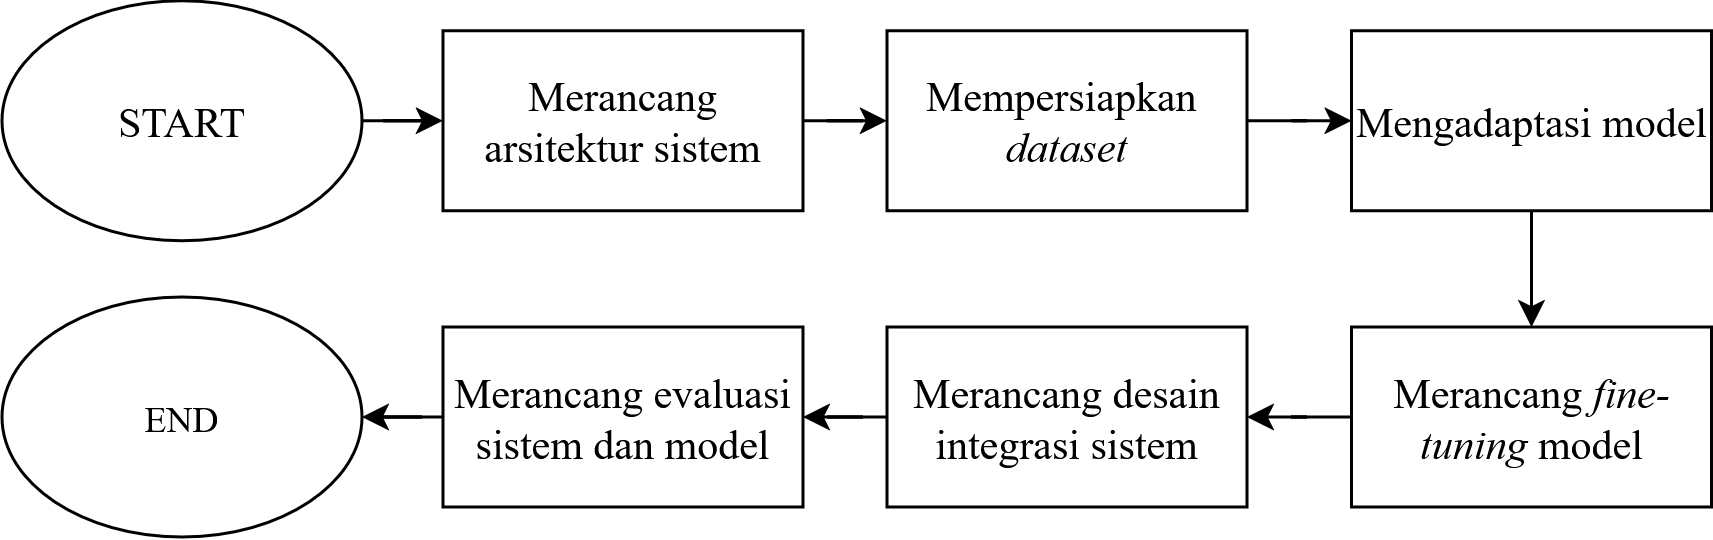
\includegraphics[width=\textwidth]{images/design-flow.png}
    \caption{Alur kerja tahapan desain sistem ekstraksi data struk dan bukti pembayaran}
    \label{fig:design-flow}
\end{figure}

\autoref{fig:design-flow} menunjukkan tahapan desain yang dilakukan dalam penelitian ini. Tahapan desain utama mencakup perancangan \emph{fine-tuning} model, perancangan konversi model, perancangan aplikasi \emph{mobile}, dan perancangan \emph{backend service} sebagai \emph{fallback mechanism}. Tahapan desain yang dihasilkan akan menjadi dasar untuk mengembangkan sistem ekstraksi data struk dan bukti pembayaran. Tahapan desain dirancang berdasarkan pada alternatif solusi yang telah diusulkan pada \autoref{sec:analisis-pemilihan-solusi} dan disesuaikan dengan tahap desain pada metodologi \dsrm.

\subsection{Perancangan \emph{Fine-Tuning} Model \donut}
\label{subsec:perancangan-fine-tuning-model}

Subbab ini menjelaskan rancangan proses \emph{fine-tuning} model \donut{} untuk tugas ekstraksi data bukti pembayaran. Perancangan ini mencakup pemilihan model dasar, konfigurasi arsitektur, desain format keluaran, strategi \emph{preprocessing} data, dan konfigurasi pelatihan untuk melakukan \emph{fine-tuning} model \donut{} pada \dataset{} yang telah dipersiapkan. Proses ini bertujuan untuk menghasilkan model yang mampu melakukan ekstraksi informasi dari bukti pembayaran dengan akurasi tinggi, serta dapat diintegrasikan ke dalam aplikasi \emph{mobile}.

\subsubsection{Pemilihan Model Dasar dan Konfigurasi Awal}
\label{subsubsec:pemilihan-model-dasar}

Model dasar yang dipilih untuk proses \emph{fine-tuning} pada \dataset{} bukti pembayaran QRIS dan transfer adalah model \donut{} yang telah di-\emph{fine-tune} pada \dataset{} CORD-v2 yang telah disediakan oleh naver-cloud-ix. Model tersebut diberi alias \donutcord. Model \donutcord{} dipilih dengan mempertimbangkan faktor-faktor berikut:

\begin{enumerate}
    \item \textbf{\emph{Domain similarity}}: Model \donutcord telah dilatih pada \dataset{} dokumen terstruktur yang memiliki kemiripan dengan struk dan bukti pembayaran dalam hal tata letak dan struktur informasi.
    \item \textbf{Pre-trained capabilities}: Model ini telah memiliki kemampuan dasar dalam memahami dokumen semi-terstruktur, sehingga dapat mempercepat proses konvergensi selama \emph{fine-tuning}.
    \item \textbf{Arsitektur optimal}: Kombinasi \swin{} \transformer{} sebagai \emph{encoder} visual dan \bart{} sebagai \emph{decoder} teks telah terbukti efektif untuk tugas \emph{Visual Document Understanding}.
\end{enumerate}

Konfigurasi awal model melibatkan ekspansi vocabulary tokenizer untuk menambahkan token khusus domain pembayaran. Penulis menambahkan 14 token khusus yang terdiri dari:
\begin{enumerate}
    \item Token pembuka dan penutup untuk setiap \emph{field}
    \begin{enumerate}
    \item \texttt{<s\_total\_amount>}, \texttt{</s\_total\_amount>}
    \item \texttt{<s\_transaction\_time>}, \texttt{</s\_transaction\_time>}
    \item \texttt{<s\_transaction\_identifier>}, \texttt{</s\_transaction\_identifier>}
    \item \texttt{<s\_type>}, \texttt{</s\_type>}
    \item \texttt{<s\_target\_name>}, \texttt{</s\_target\_name>}
    \item \texttt{<s\_application>}, \texttt{</s\_application>}
    \end{enumerate}
    \item Token \emph{task identifier}~\\ \texttt{<s\_payment\_proof>}, \texttt{</s\_payment\_proof>}
\end{enumerate}

Ekspansi vocabulary ini memerlukan penyesuaian dimensi embedding layer pada decoder dan konfigurasi ulang parameter \texttt{decoder\_start\_token\_id} untuk memastikan model memulai generasi dengan token task yang tepat.

\subsubsection{Desain Format Keluaran Terstruktur}
\label{subsubsec:desain-format-keluaran}

Penulis merancang format keluaran terstruktur yang memungkinkan ekstraksi informasi yang konsisten dan dapat diparsing secara otomatis. Format yang dirancang menggunakan markup berbasis XML dengan struktur hierarkis sebagai berikut:

\begin{verbatim}
<s_payment_proof>
<s_total_amount>nilai_total</s_total_amount>
<s_transaction_time>waktu_transaksi</s_transaction_time>
<s_transaction_identifier>id_transaksi</s_transaction_identifier>
<s_type>jenis_transaksi</s_type>
<s_target_name>nama_tujuan</s_target_name>
<s_application>aplikasi_pembayaran</s_application>
</s_payment_proof>
\end{verbatim}

Desain ini memiliki beberapa keunggulan:
\begin{enumerate}
    \item \textbf{Struktur yang jelas}: Setiap field memiliki delimiter yang eksplisit, memudahkan parsing dan validasi keluaran.
    \item \textbf{Fleksibilitas}: Field yang tidak terdeteksi dapat diabaikan tanpa merusak struktur keseluruhan.
    \item \textbf{Konsistensi}: Format yang tetap memungkinkan evaluasi otomatis dan sistem monitoring.
    \item \textbf{Extensibility}: Struktur dapat diperluas untuk menambahkan field baru tanpa mengubah parser yang ada.
\end{enumerate}

Token \texttt{<s\_payment\_proof>} berfungsi sebagai task prompt yang memberikan konteks kepada model bahwa tugas yang dijalankan adalah ekstraksi informasi dari dokumen pembayaran, berbeda dari tugas lain seperti ekstraksi dokumen umum.

\subsubsection{Strategi Preprocessing Data}
\label{subsubsec:strategi-preprocessing-data}

Mengingat karakteristik data metadata yang berpotensi mengalami korupsi atau format yang tidak konsisten, penulis merancang strategi preprocessing yang robust dengan beberapa tahapan:

\paragraph{Pembersihan Metadata}
Penulis mengimplementasikan parser multi-tahap untuk menangani file metadata yang berformat JSONL tetapi mengalami masalah formatting:
\begin{enumerate}
    \item \textbf{Parser Array JSON}: Mencoba parsing sebagai array JSON lengkap setelah menambahkan delimiter koma.
    \item \textbf{Parser Line-by-Line}: Jika gagal, melakukan parsing objek JSON per baris dengan tracking brace count untuk rekonstruksi objek yang terpisah.
    \item \textbf{Error Recovery}: Menangani karakter khusus dan trailing commas yang dapat menyebabkan parsing error.
\end{enumerate}

\paragraph{Pencocokan File Gambar}
Sistem pencarian file gambar yang fleksibel diimplementasikan untuk mengatasi inkonsistensi penamaan file:
\begin{itemize}
    \item Pencocokan direct path
    \item Pencocokan case-insensitive untuk handling variasi kapitalisasi
    \item Pencocokan dengan berbagai ekstensi gambar (.jpg, .jpeg, .png)
    \item Pencocokan partial untuk nama file tanpa ekstensi
\end{itemize}

\paragraph{Validasi dan Pembersihan Data}
Setiap sample data divalidasi untuk memastikan:
\begin{itemize}
    \item Keberadaan file gambar yang valid
    \item Kelengkapan ground truth annotation
    \item Konsistensi format field value (normalisasi spasi internal)
    \item Handling nilai null atau kosong
\end{itemize}

\subsubsection{Konfigurasi Pelatihan dan Optimisasi}
\label{subsubsec:konfigurasi-pelatihan}

Penulis merancang konfigurasi pelatihan yang mempertimbangkan keterbatasan sumber daya komputasi sambil memaksimalkan kualitas hasil \emph{fine-tuning}:

\paragraph{Hyperparameter Selection}
\begin{itemize}
    \item \textbf{Learning Rate}: 3e-5, dipilih sebagai trade-off antara kecepatan konvergensi dan stabilitas pelatihan
    \item \textbf{Batch Size}: 1 per device dengan gradient accumulation 8 steps, memberikan effective batch size 8
    \item \textbf{Epochs}: 40 dengan early stopping patience 3 untuk mencegah overfitting
    \item \textbf{Weight Decay}: 0.01 untuk regularisasi model
\end{itemize}

\paragraph{Optimisasi Memori}
Untuk mengatasi keterbatasan memori GPU, penulis mengimplementasikan beberapa teknik optimisasi:
\begin{enumerate}
    \item \textbf{Mixed Precision Training}: Menggunakan FP16 untuk mengurangi penggunaan memori hingga 50\%
    \item \textbf{Gradient Checkpointing}: Menukar komputasi tambahan dengan penghematan memori
    \item \textbf{Memory Management}: Disable pin memory dan multiprocessing pada dataloader
    \item \textbf{Garbage Collection}: Pembersihan cache CUDA secara eksplisit
\end{enumerate}

\paragraph{Data Collation Strategy}
Penulis merancang custom collation function yang menangani:
\begin{itemize}
    \item Forcing decoder input dengan task start token
    \item Proper label masking untuk padding tokens (-100 untuk ignore dalam loss calculation)
    \item Batch consistency handling untuk samples dengan ukuran berbeda
\end{itemize}

\subsubsection{Desain Sistem Evaluasi dan Monitoring}
\label{subsubsec:desain-evaluasi-monitoring}

Sistem evaluasi dirancang untuk memberikan insight mendalam tentang performa model pada level field individual maupun keseluruhan:

\paragraph{Metrik Evaluasi}
\begin{enumerate}
    \item \textbf{Field-wise Accuracy}: Akurasi ekstraksi untuk setiap field secara terpisah menggunakan regex parsing
    \item \textbf{Overall Sequence Accuracy}: Persentase prediksi yang tepat secara keseluruhan
    \item \textbf{Partial Match Analysis}: Evaluasi komponen-komponen yang benar meskipun keseluruhan prediksi salah
\end{enumerate}

\paragraph{Real-time Monitoring}
Penulis mengimplementasikan callback monitoring yang memberikan feedback real-time:
\begin{itemize}
    \item Sample prediction display setiap 5 epoch
    \item Progress tracking dengan tqdm integration
    \item Automatic model evaluation pada akhir setiap epoch
    \item Best model saving berdasarkan validation loss
\end{itemize}

\paragraph{Prediction Post-processing}
Sistem pembersihan output yang menangani:
\begin{itemize}
    \item Duplikasi start tokens
    \item Spasi berlebih dalam field values
    \item Normalisasi format output untuk konsistensi
\end{itemize}

\subsubsection{Strategi Robustness dan Generalisasi}
\label{subsubsec:strategi-robustness}

Untuk meningkatkan kemampuan generalisasi model pada berbagai variasi dokumen pembayaran, penulis merancang beberapa strategi:

\paragraph{Error Handling Mechanism}
\begin{enumerate}
    \item \textbf{Graceful Degradation}: Jika sample mengalami error processing, sistem menggunakan dummy sample untuk menjaga training continuity
    \item \textbf{Tokenization Safety}: Validasi range token ID untuk mencegah out-of-vocabulary errors
    \item \textbf{Decode Error Recovery}: Safe decoding dengan fallback ke empty string untuk token yang tidak valid
\end{enumerate}

\paragraph{Data Quality Assurance}
\begin{itemize}
    \item Filtering sample dengan ground truth yang tidak lengkap
    \item Validasi format gambar dan konversi otomatis ke RGB
    \item Normalisasi nilai field untuk konsistensi (handling numerical values, date formats)
\end{itemize}

\paragraph{Generation Configuration}
Konfigurasi generation yang dioptimalkan untuk task-specific requirements:
\begin{itemize}
    \item \textbf{Beam Search}: Menggunakan 4 beams untuk balance antara quality dan speed
    \item \textbf{Length Control}: Max length 512 tokens dengan early stopping
    \item \textbf{Repetition Prevention}: N-gram repetition penalty dan bad words filtering
    \item \textbf{Token Constraints}: Proper EOS dan padding token handling
\end{itemize}

Rancangan \emph{fine-tuning} ini dirancang untuk menghasilkan model yang robust, akurat, dan dapat diandalkan untuk ekstraksi informasi dari berbagai jenis struk dan bukti pembayaran yang umum digunakan di Indonesia. Implementasi yang telah dirancang akan dijelaskan lebih lanjut pada \autoref{subsec:fine-tuned-model}.

\subsection{Perancangan Konversi dan Kompresi Model}
\label{subsec:perancangan-konversi-dan-kompresi-model}

 Proses konversi dan kompresi model \donut{} dari format PyTorch \emph{orisinil} ke format yang \emph{optimized} untuk \emph{on-device inference}. Proses tersebut diperlukan untuk mencapai tujuan model yang dapat digunakan pada perangkat \emph{mobile} Android. Subbab ini menjelaskan pendekatan yang digunakan untuk konversi model ke format \emph{Open Neural Network Exchange} (ONNX) dan strategi kompresi yang akan diterapkan pada model.

\subsubsection{Perancangan Konversi dan Kompresi Model \donut{} ke ONNX}
\label{subsubsec:strategi-konversi-onnx}

\emph{Open Neural Network Exchange} (ONNX) dipilih sebagai target format konversi utama karena memberikan keunggulan dalam hal portabilitas lintas \emph{platform} dan optimasi \emph{inference}. ONNX menyediakan dukungan luas untuk berbagai \emph{framework} dan perangkat keras, sehingga memungkinkan integrasi yang lebih baik dengan \emph{platform mobile}. Perubahan format menuju \onnx{} merupakan langkah penting untuk memastikan model dapat dioptimalkan.

Arsitektur model \donut{} yang berbasis \textit{VisionEncoderDecoderModel} bukan merupakan arsitektur yang umum untuk dikonversi, sehingga konversi ke ONNX memerlukan pendekatan yang lebih kompleks dibandingkan model lainnya. \onnx{} telah menyediakan \emph{export tool}{}\footnote{\url{https://huggingface.co/spaces/onnx/export}} yang dapat digunakan untuk mengonversi model PyTorch ke format ONNX. \emph{Export tool} ini akan digunakan untuk melakukan konversi model \donut{} ke format ONNX dan model tersebut yang akan digunakan sebagai dasar untuk kompresi model lebih lanjut. 

\subsubsection{Strategi Kompresi dan Kuantisasi Model}
\label{subsubsec:strategi-kompresi-dan-kuantisasi-model}

Model \donut{} yang telah dikonversi ke format \onnx{} akan melalui tahap kompresi untuk mengurangi ukuran model dan meningkatkan kecepatan inferensi pada perangkat mobile. Kompresi ini penting untuk memastikan model dapat berjalan efisien pada perangkat dengan keterbatasan sumber daya, seperti pada perangkat Android. Metode yang digunakan untuk kompresi dan kuantisasi adalah \emph{Dynamic Quantization}. \emph{Dynamic quantization} dipilih sebagai pendekatan utama untuk melakukan kompresi dan kuantisasi model \donut. Metode \emph{Dynamic Quantization} yang dapat diterapkan adalah FP16, INT8, dan UINT8. Pendekatan ini memungkinkan model untuk tetap mempertahankan akurasi yang tinggi sambil mengurangi ukuran model secara signifikan.


\subsection{Perancangan Evaluasi Model}
\label{subsec:perancangan-evaluasi-model}

\subsection{Perancangan \emph{Backend Service} sebagai \emph{Fallback Mechanism}}
\label{subsec:perancangan-fallback-mechanism}   

\subsection{Perancangan Aplikasi \emph{Mobile}}
\label{subsec:perancangan-aplikasi-mobile}



\section{Hasil Desain}
\label{sec:hasil-desain}



\chapter{Penutup}

\section{Kesimpulan}
\blindtext

\section{Saran}
\blindtext

\chapter{Kesimpulan dan Saran}

\section{Kesimpulan}
\label{sec:kesimpulan}
Tugas akhir ini bertujuan untuk mengembangkan sistem pencatatan pengeluaran berbasis \emph{mobile} yang dapat membantu pengguna, yaitu Gen Z, dalam mencatat pengeluaran mereka dengan lebih mudah. Sistem ini menggunakan model \donut{} untuk mengekstrak informasi penting dari gambar bukti pembayaran dan menyimpannya dalam format yang terstruktur untuk kemudian dapat ditampilkan kepada pengguna. Hasil evaluasi sistem menunjukkan bahwa aplikasi TrackMyBills \textbf{berhasil} memenuhi seluruh evaluasi yang dilakukan, yaitu dari pengujian fungsionalitas, pengujian kinerja model, dan pengujian pengalaman pengguna. 

Pengujian fungsionalitas \emph{berhasil} menunjukkan bahwa seluruh skenario pengujian dapat dijalankan dengan baik dan sesuai dengan yang diharapkan. Pengujian pengalaman pengguna menunjukkan bahwa aplikasi memiliki tingkat kepuasan pengguna yang baik, dengan nilai SUS di angka \textbf{71,83} rata-rata di atas ambang batas nilai SUS, yaitu pada \textbf{68}. Hal ini menunjukkan bahwa aplikasi dapat memberikan pengalaman pengguna yang baik dan memenuhi kebutuhan pengguna dalam mencatat pengeluaran mereka.

Pengujian kinerja model menunjukkan bahwa kedua model yang digunakan, yaitu \donut{} yang di \emph{fine-tune} pada \dataset{} CORD-v2 (\emph{base model}) dan \donut{} yang di \emph{fine-tune} pada \dataset{} QRIS-TF (\emph{custom model}), menunjukkan hasil yang memuaskan dengan nilai \accuracy, \precision, \recall, \fscore, dan \mcer{} yang melewati standar yang telah ditetapkan. \emph{Base model} menunjukkan angka \accuracy{} \textbf{73,43\%}, \precision{} \textbf{90,53\%}, \recall{} \textbf{79,53\%}, \fscore{} \textbf{84,68\%}, dan \mcer{} \textbf{18,85\%}. \emph{Custom model} menunjukkan angka \accuracy{} \textbf{68,78\%}, \precision{} \textbf{100\%}, \recall{} \textbf{68,78\%}, \fscore{} \textbf{81,50\%}, dan \mcer{} \textbf{17,20\%}. Hal ini menunjukkan bahwa model dapat mengenali dan mengekstrak informasi penting dari gambar struk dengan hasil yang baik. 

\section{Saran}
\label{sec:saran}
Meskipun sistem TrackMyBills telah menunjukkan kinerja yang baik dan mendapatkan umpan balik positif dari pengguna, masih ada beberapa area yang dapat ditingkatkan. Kinerja model \donut{} masih dapat ditingkatkan dengan melatih model pada data yang lebih beragam dan representatif, terutama untuk dokumen pembayaran QRIS dan transfer. 

\datasetfl{} CORD-v2 yang digunakan untuk \emph{fine-tuning} model \donut{} belum dapat memberikan kebebasan kepada model untuk memahami dokumen secara holistik sehingga model masih memerlukan \emph{cropping} pada gambar bukti pembayaran sebelum diekstrak. Penelitian selanjutnya dapat membuat \dataset{} seperti CORD-v2 tanpa menghilangkan sebagian informasi yang tidak relevan dan melatihnya pada model \donut{} untuk menghilangkan kebutuhan pemotongan gambar.

TrackMyBills masih menggunakan dua model yang berbeda untuk menangani dua kasus yang berbeda, yaitu dokumen pembayaran QRIS dan transfer serta struk pembayaran. Penelitian selanjutnya dapat mencoba untuk menggunakan satu model yang dapat menangani kedua jenis dokumen tersebut dengan \emph{task prompt} yang sesuai untuk masing-masing jenis dokumen untuk mengurangi kompleksitas sistem yang dibangun.

Sistem TrackMyBills masih dapat dikembangkan lebih lanjut dengan menambahkan fitur-fitur penting, sebagai berikut.
\begin{enumerate}
    \item Integrasi dengan layanan perbankan\\~ Fitur ini akan memudahkan pengguna dalam mencatat pengeluaran mereka tanpa perlu mengunggah bukti pembayaran secara manual.
    \item Melihat detail transaksi lampau dan membuat perubahan\\~ Fitur ini akan memungkinkan pengguna untuk mengelola dan memperbaiki data transaksi yang telah dicatat sebelumnya.
    \item Integrasi dengan sistem basis data \emph{cloud}\\~
    Fitur ini akan memungkinkan pengguna untuk mengakses data mereka dari berbagai perangkat dan memastikan data tetap aman meskipun gawai pengguna hilang atau rusak.
\end{enumerate}
%---------------------------------------------------------------%

% Daftar pustaka
\printbibliography{}

% Setting judul lampiran
\titlespacing*{\chapter}{0pt}{0pt}{0pt}
\titlespacing*{\section}{0pt}{0pt}{*1}

% Setting judul anak lampiran - maintain 12pt consistency
\titleformat*{\section}{\normalfont\normalsize\bfseries}

\appendix

\chapter{Tautan Penting}
\label{chapter:tautan-penting}

\section{Tautan \emph{Script} Fine-Tuning}
\href{https://www.kaggle.com/code/vincentfranstyo/fine-tuned-for-qris-tf/}{https://www.kaggle.com/code/vincentfranstyo/fine-tuned-for-qris-tf/}

\section{Tautan \emph{Script} Evaluasi \emph{Base Model}}
\href{https://www.kaggle.com/code/vincentfranstyo/donut-fine-tuned-on-cord-v2-evaluation/}{https://www.kaggle.com/code/vincentfranstyo/donut-fine-tuned-on-cord-v2-evaluation/}

\section{Tautan \emph{Script} Evaluasi \emph{Custom Model}}
\href{https://www.kaggle.com/code/vincentfranstyo/qris-tf-eval-new}{https://www.kaggle.com/code/vincentfranstyo/qris-tf-eval-new}

\section{Tautan Repositori Kode Aplikasi \emph{Mobile} TrackMyBills}
\href{https://github.com/FYP-TrackMyBills/TrackMyBills}{https://github.com/FYP-TrackMyBills/TrackMyBills}

\section{Tautan Repositori Kode Layanan \emph{Backend} DonutAPI}
\href{https://github.com/FYP-TrackMyBills/Donut-Backend}
{https://github.com/FYP-TrackMyBills/Donut-Backend}

\section{Tautan Survei Evaluasi Pengguna}
\href{https://forms.gle/LwDiEJtcAL2gKyBfA}{https://forms.gle/LwDiEJtcAL2gKyBfA}

\section{Tautan Hasil Survei Pengguna}
\href{https://docs.google.com/spreadsheets/d/1a2Q1Kio0whC7-fwUD3y7AQzv5Cw0PaTOwEdsp9prtck/edit?resourcekey=&gid=529123852#gid=529123852}{Google Sheets: Hasil Survei Pengguna}
\chapter{Tangkapan Layar Antarmuka}
\label{chapter:tangkapan-layar-antarmuka}

\begin{tabular}{lll}
    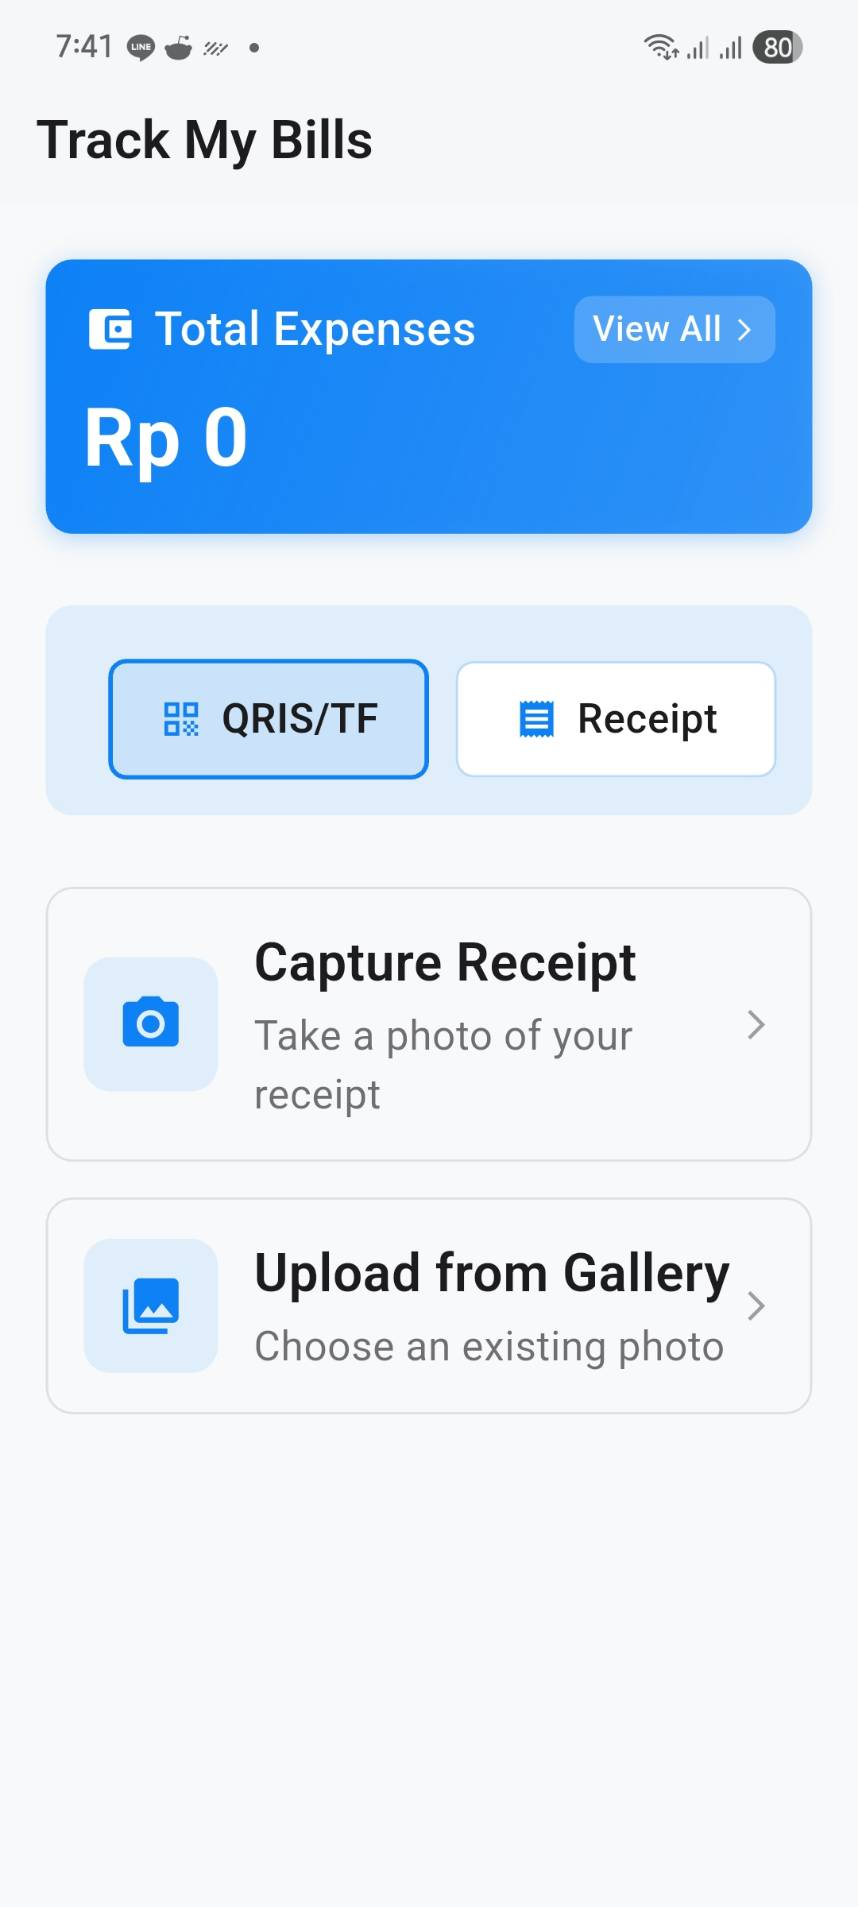
\includegraphics[width=0.33\textwidth]{images/UI/choose-document-2.jpg} &
    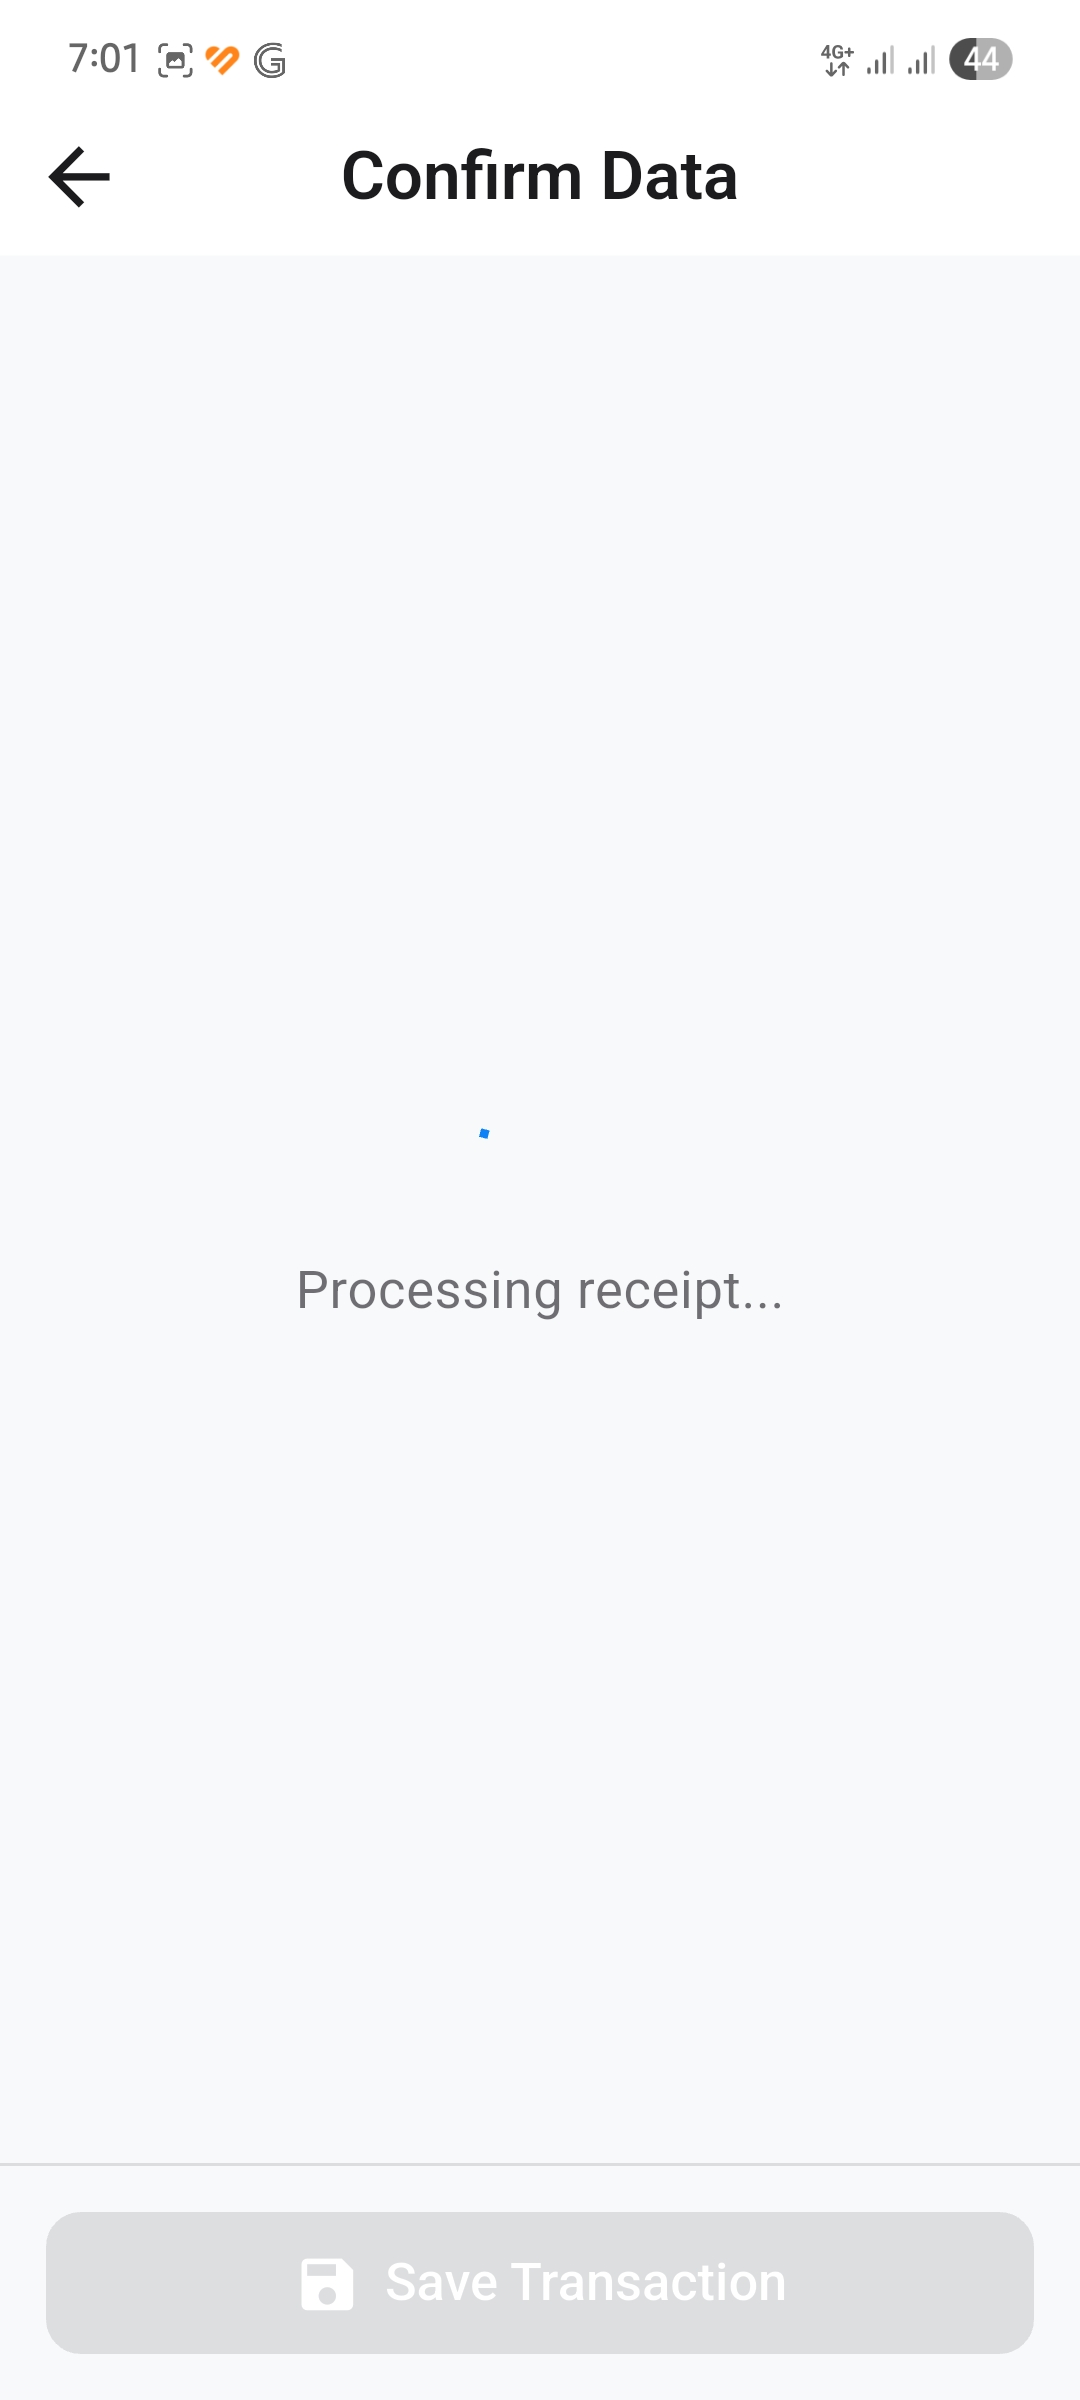
\includegraphics[width=0.33\textwidth]{images/UI/extracting.jpg} &
    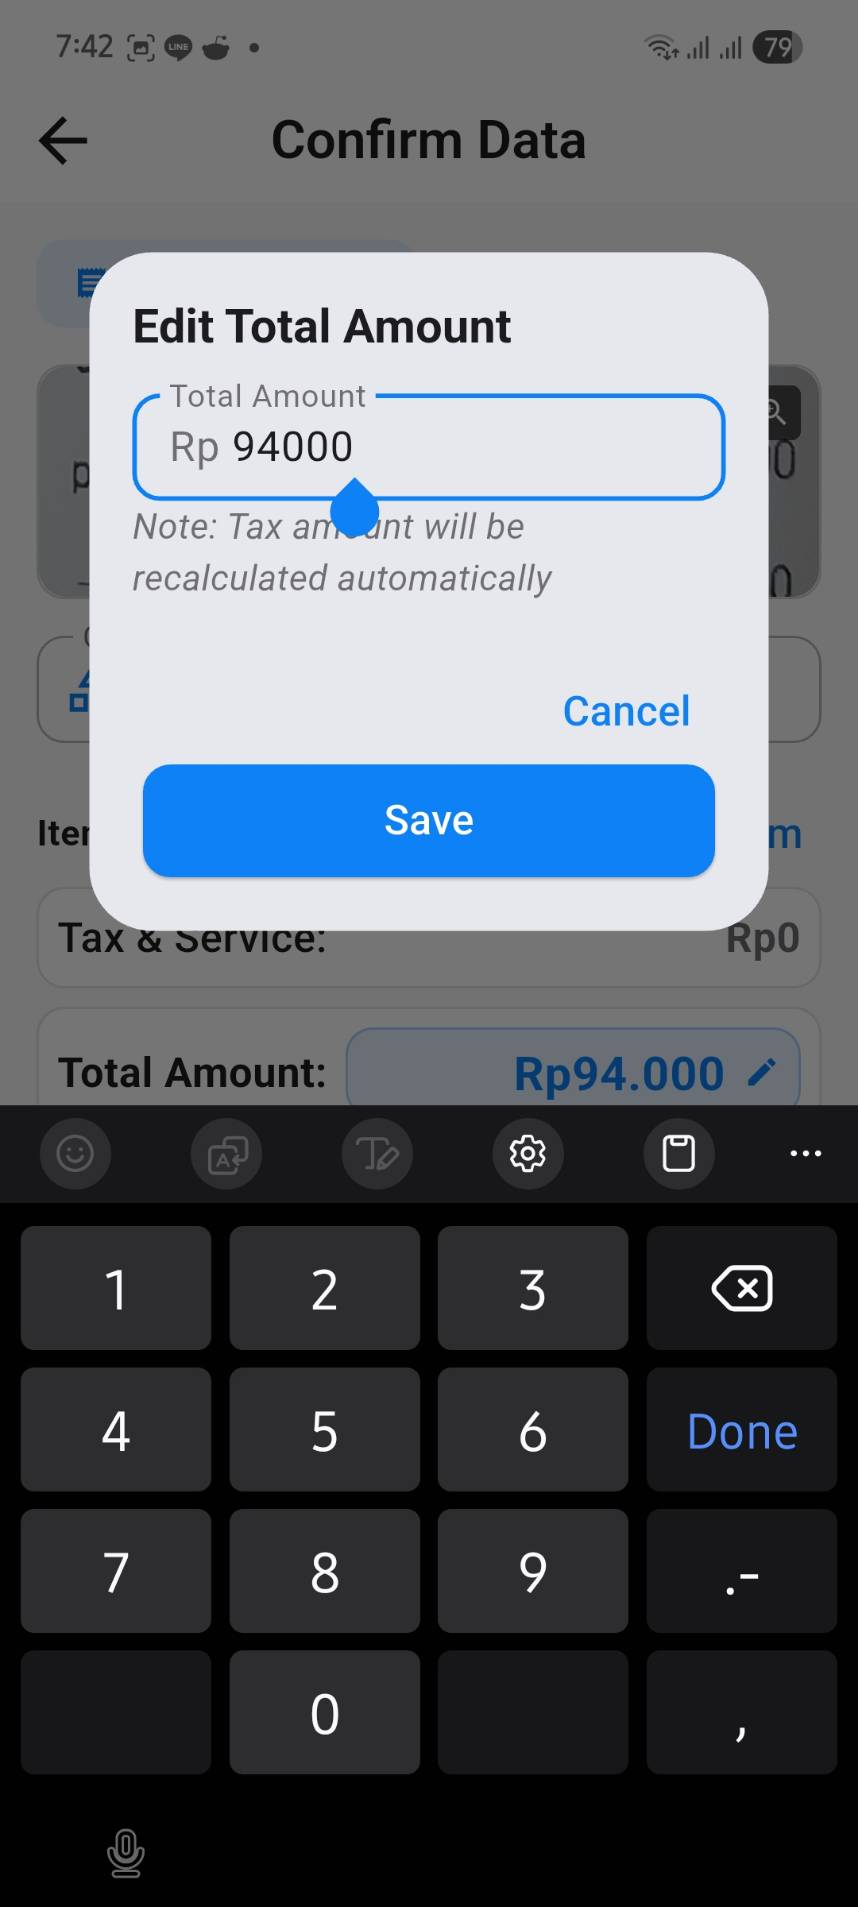
\includegraphics[width=0.33\textwidth]{images/UI/struk-edit-ta.jpg}
    \\
    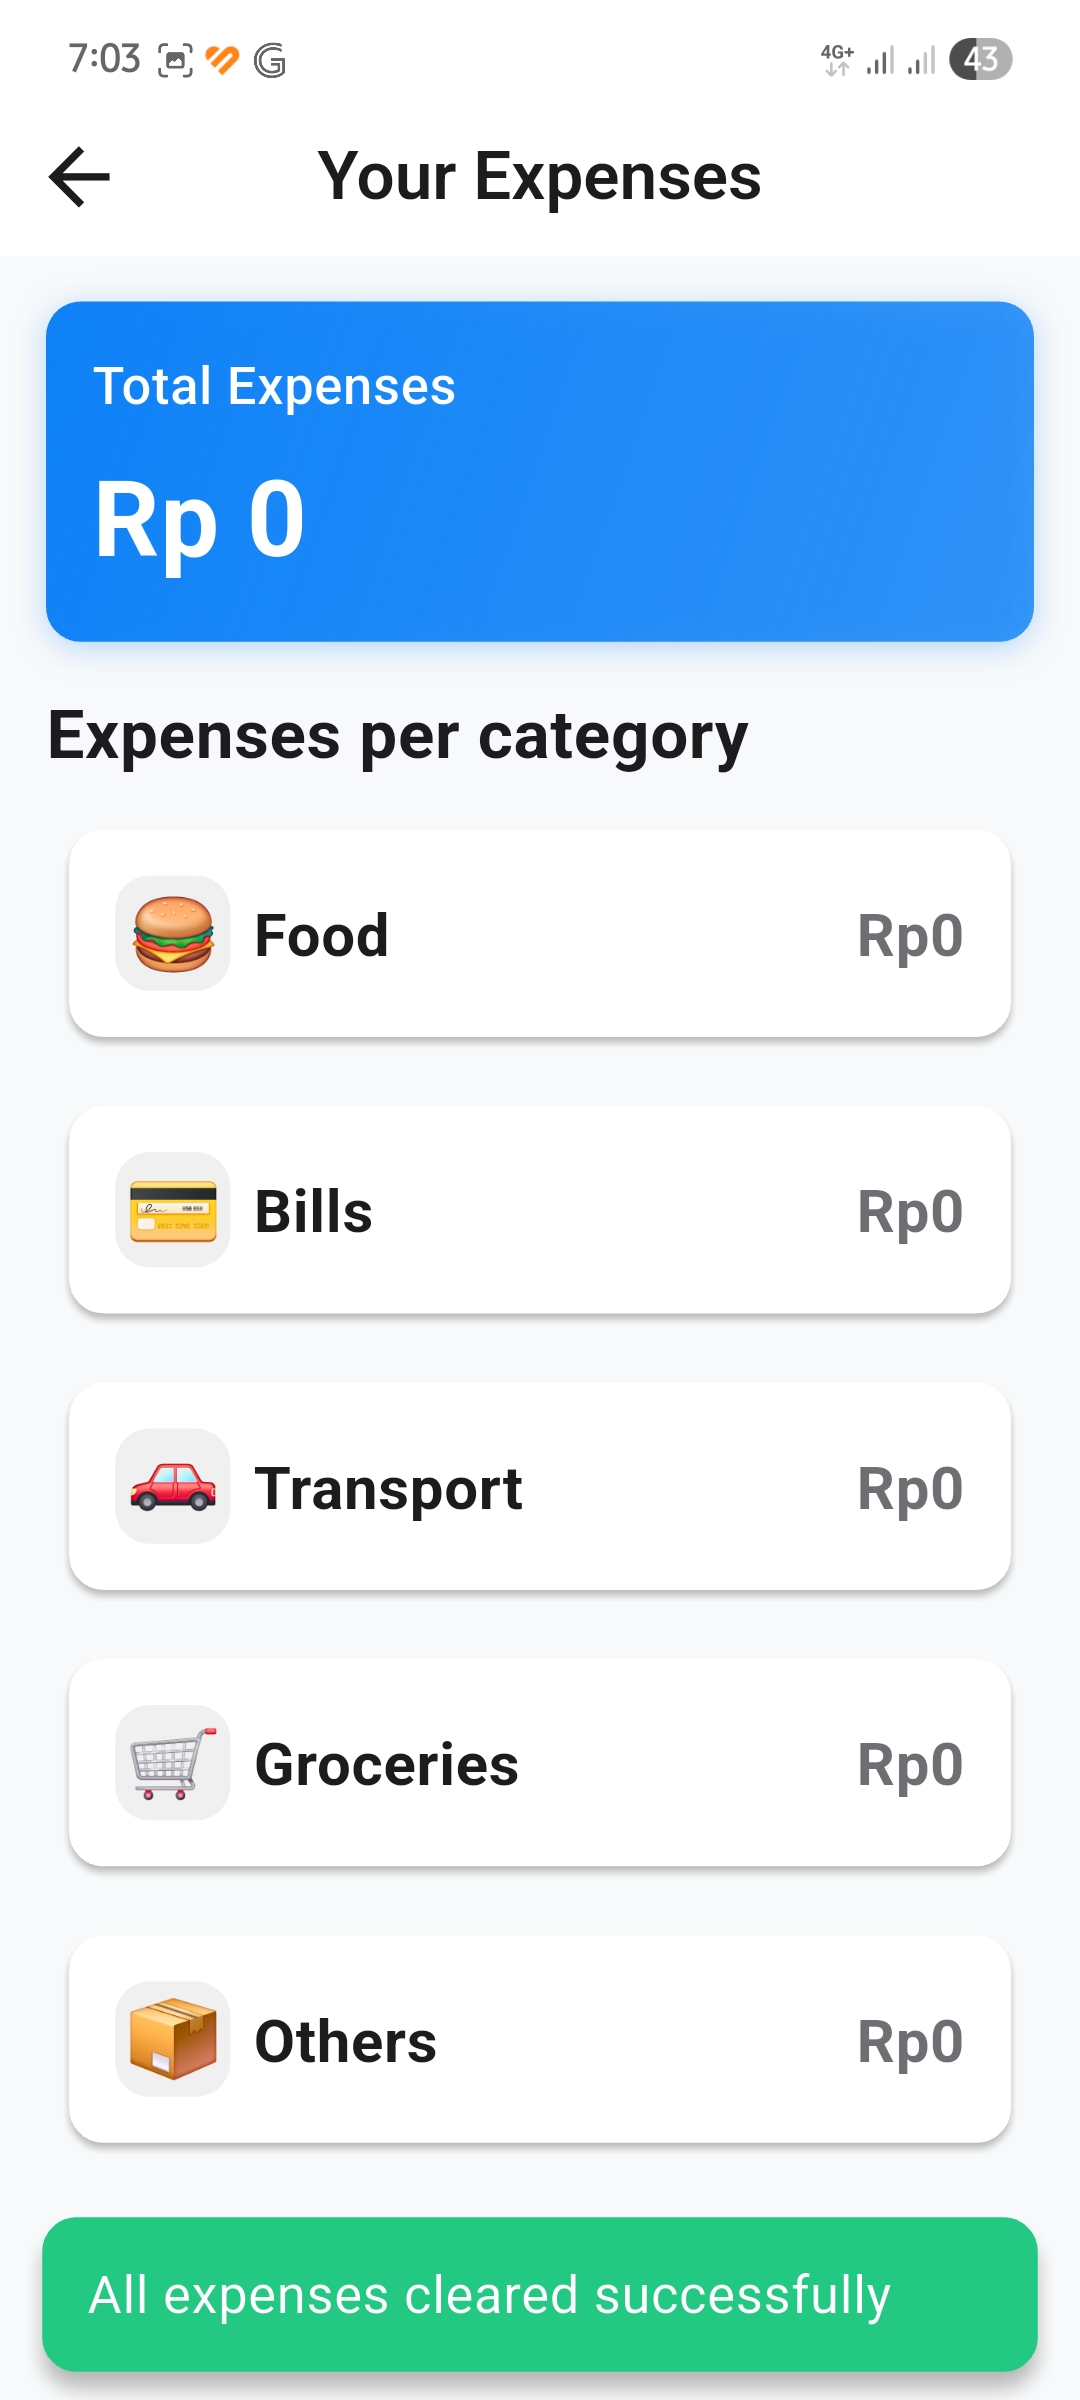
\includegraphics[width=0.33\textwidth]{images/UI/expense-0.jpg} &
    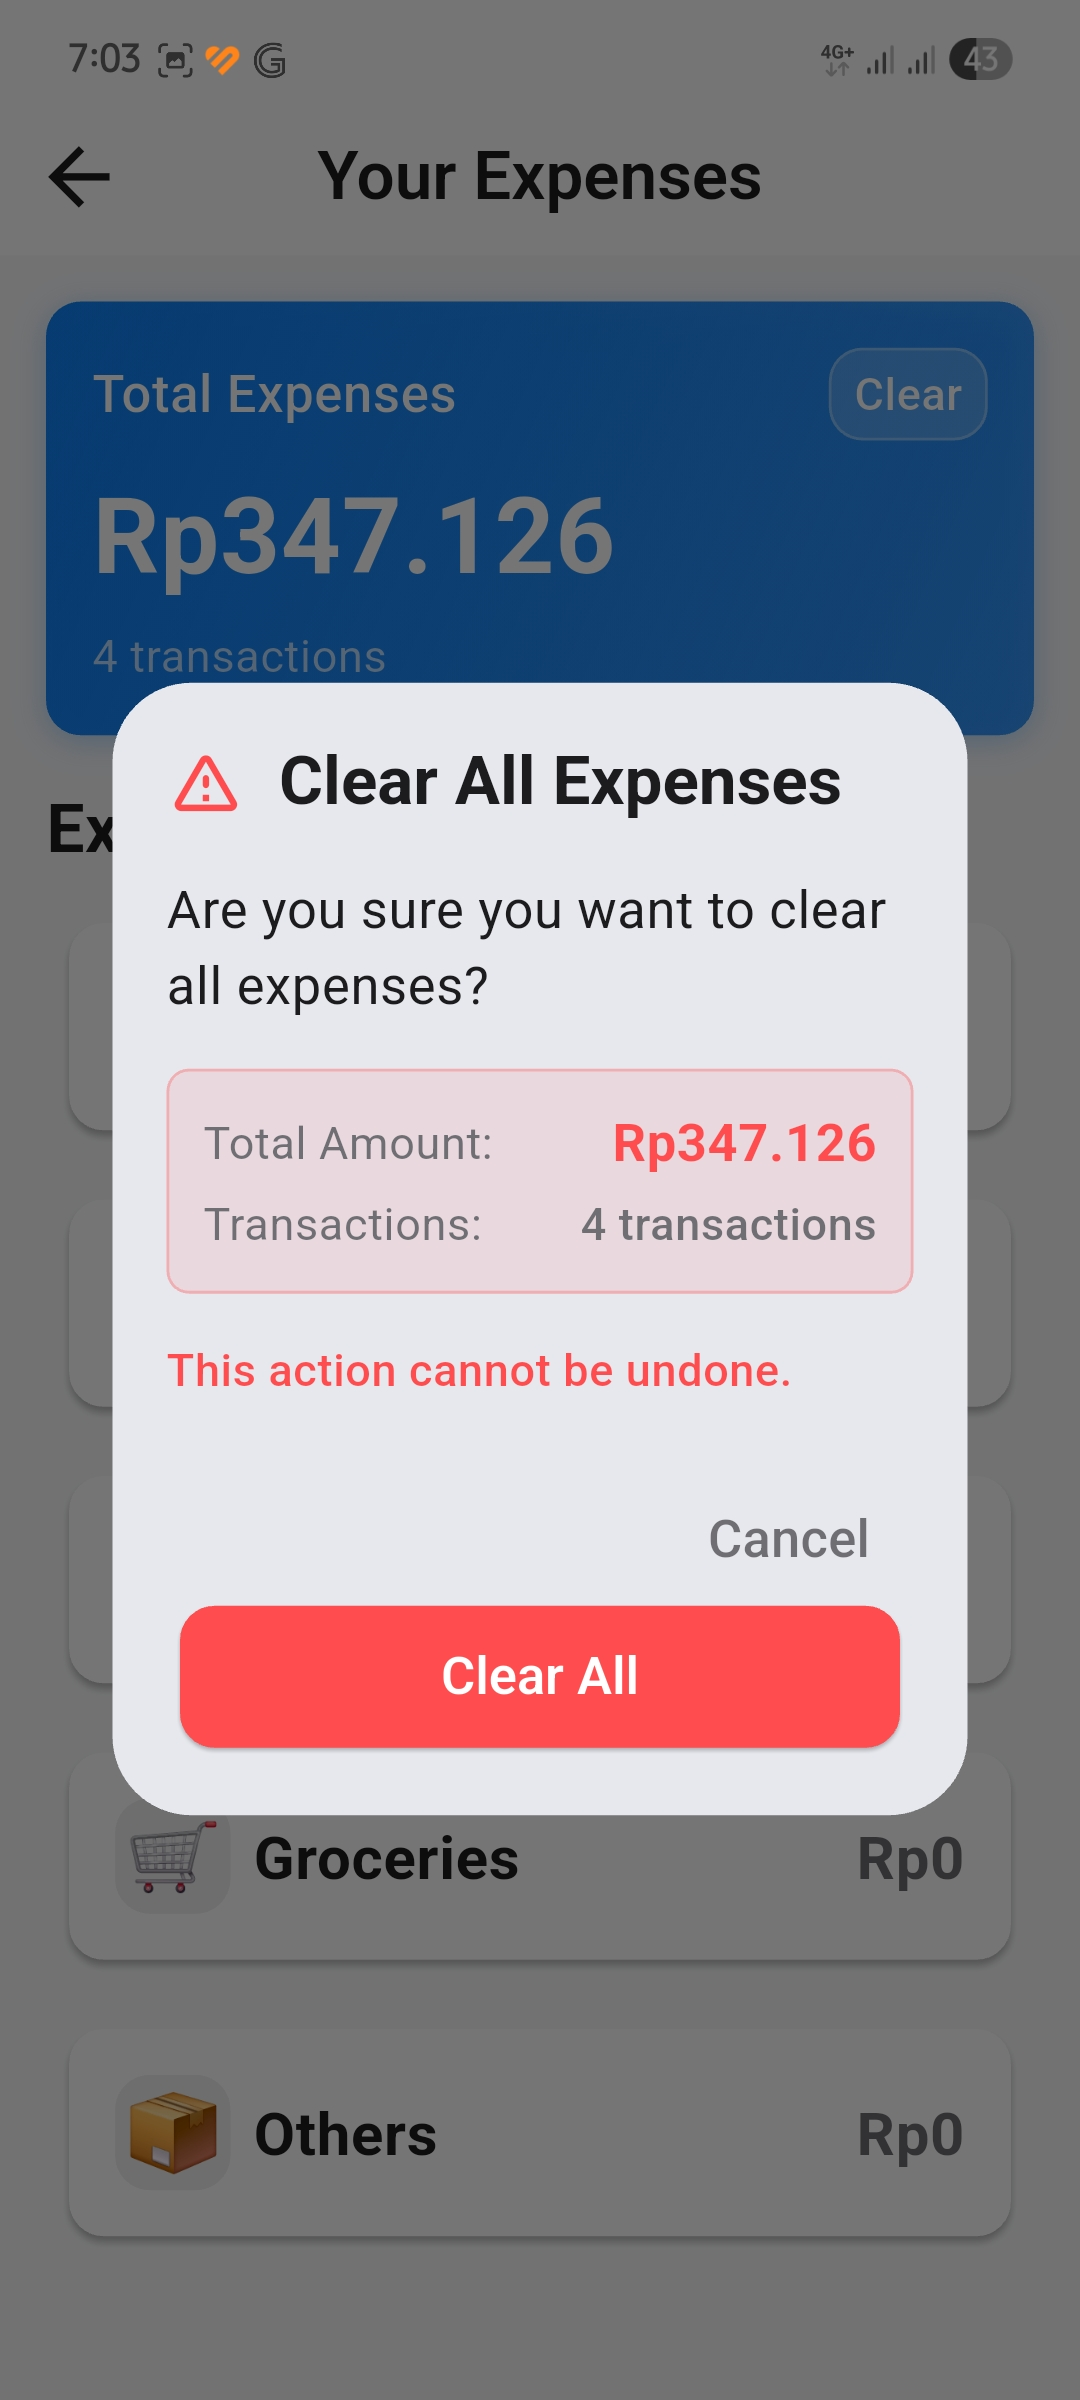
\includegraphics[width=0.33\textwidth]{images/UI/expense-clear.jpg} &
    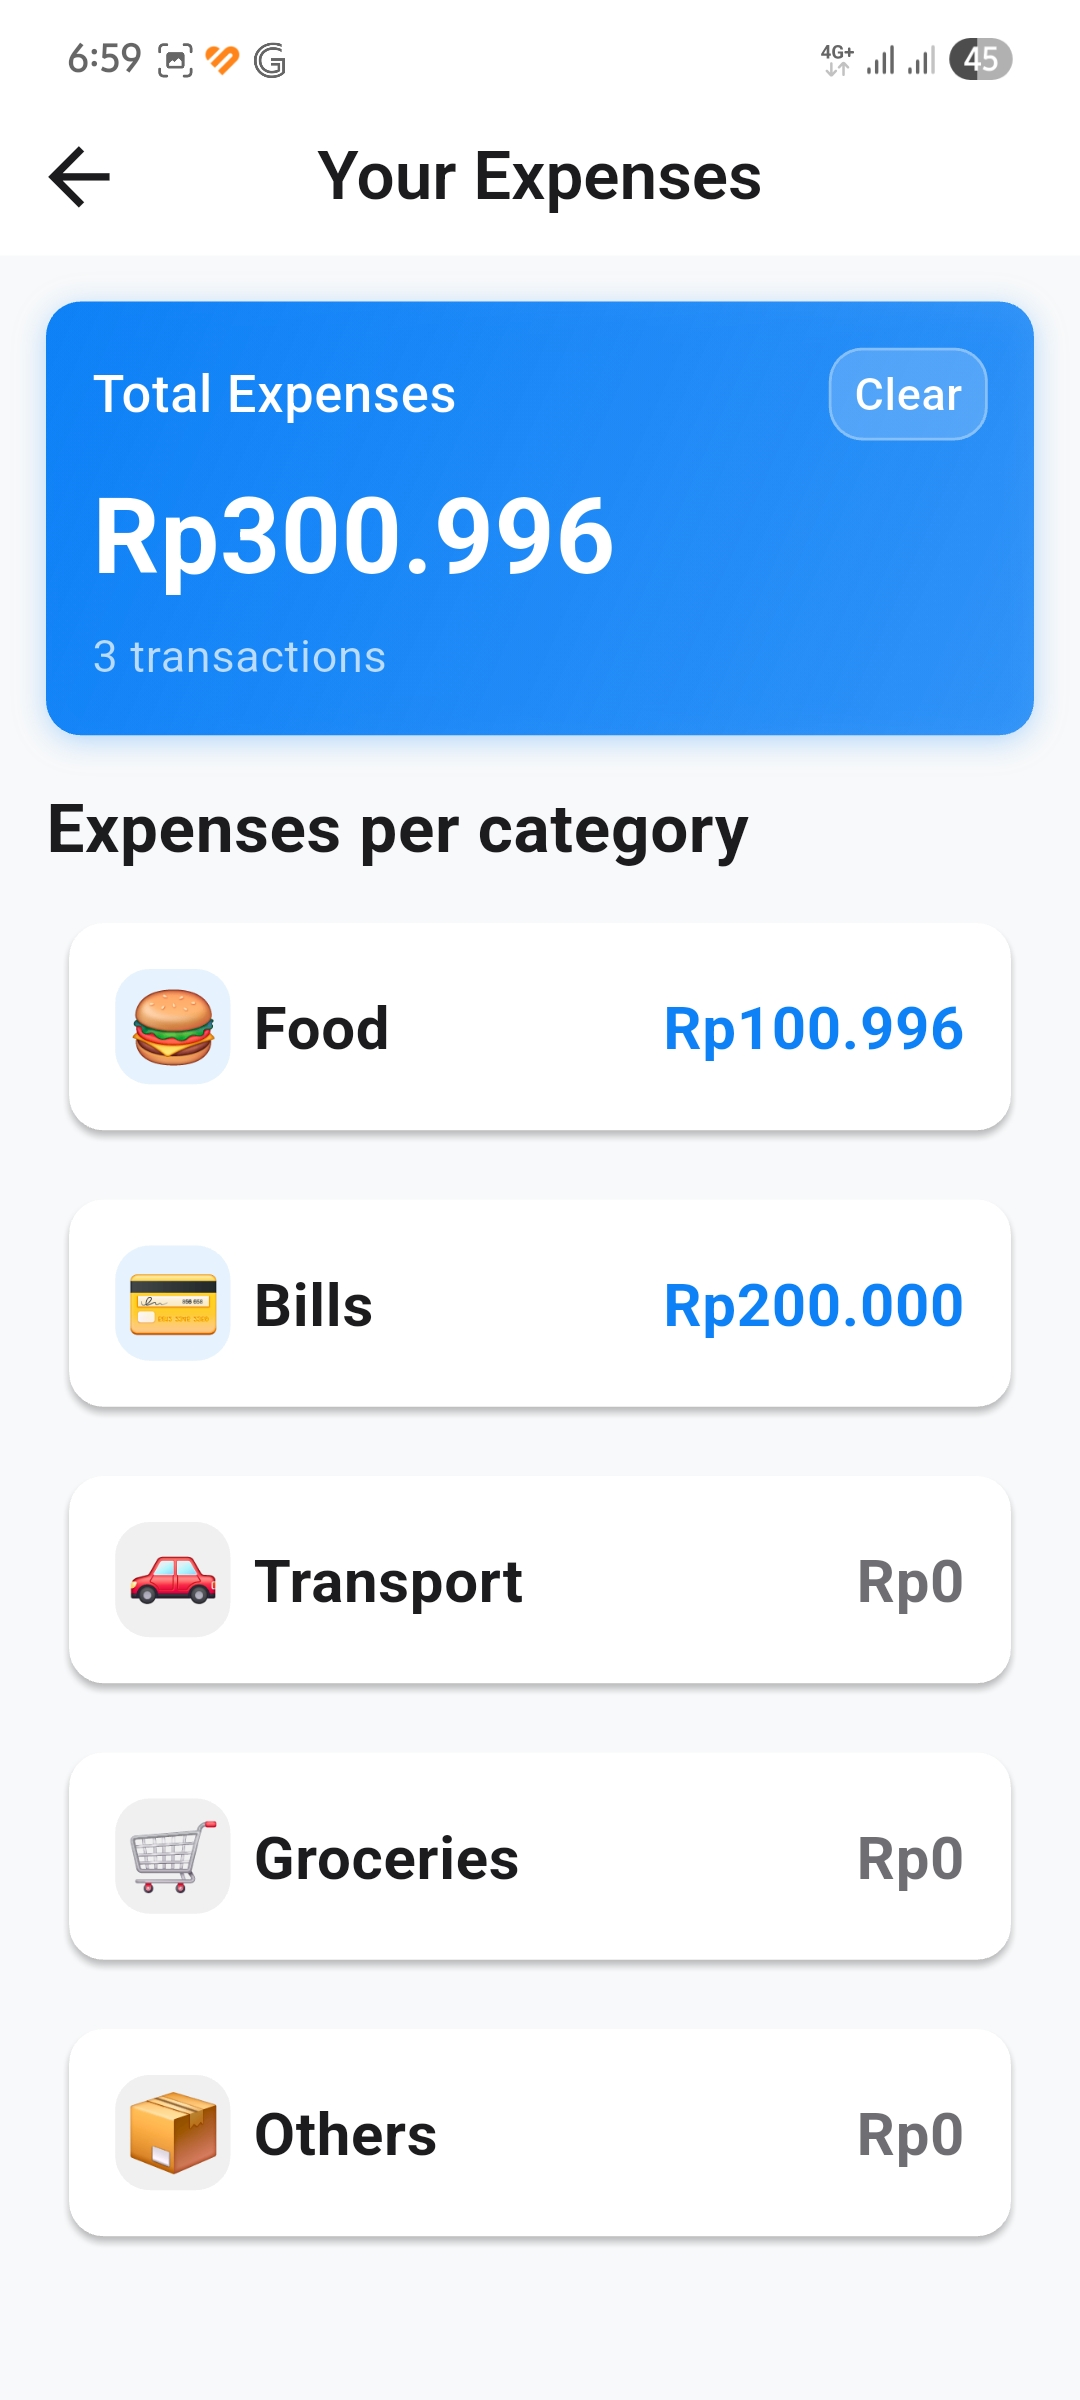
\includegraphics[width=0.33\textwidth]{images/UI/expense.jpg} \\
\end{tabular}

\begin{tabular}{lll}
    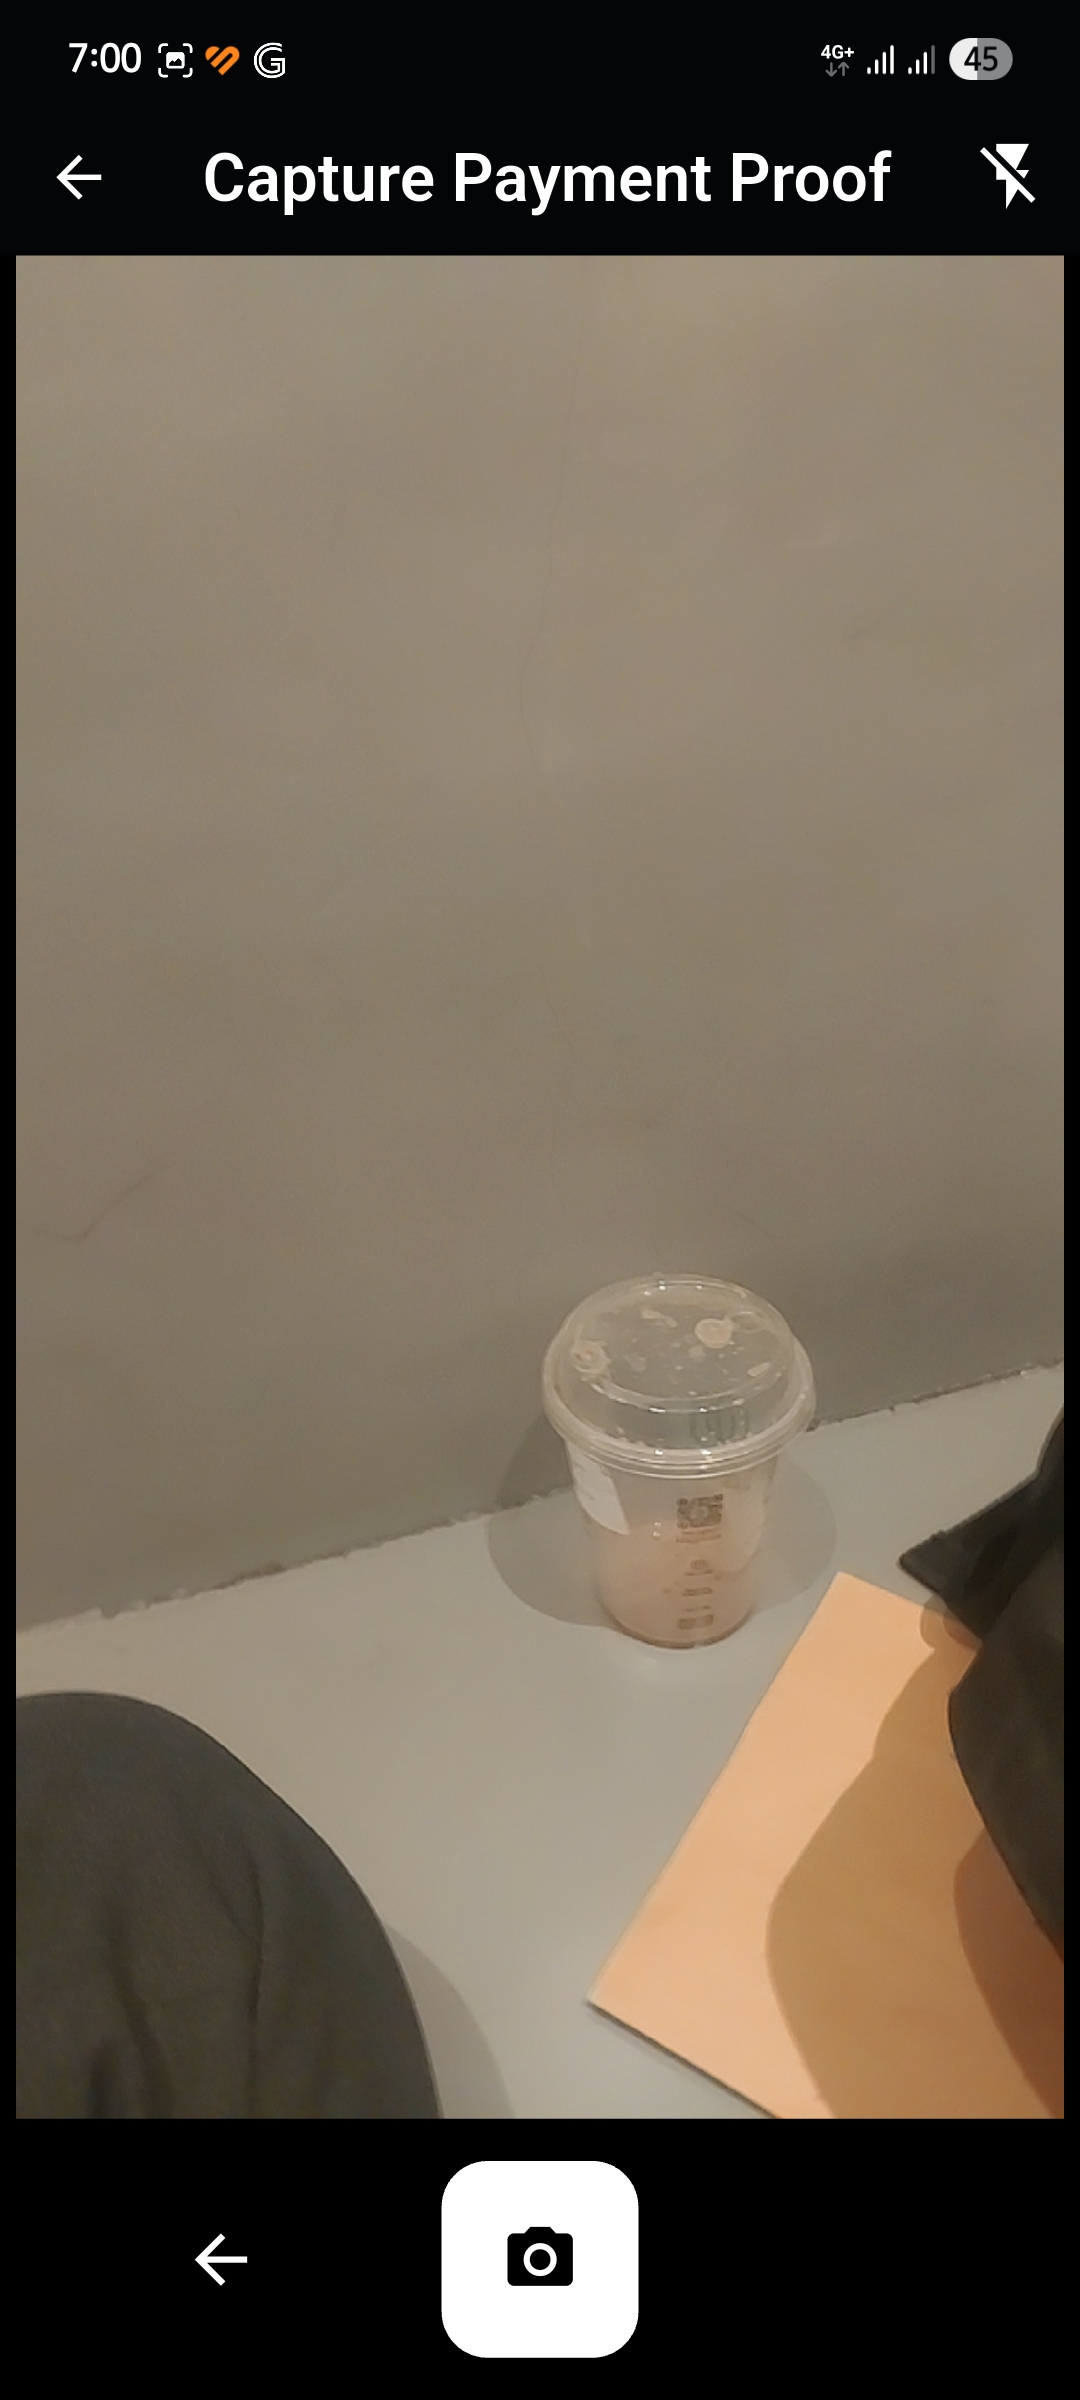
\includegraphics[width=0.33\textwidth]{images/UI/qris-cam.jpg} &
    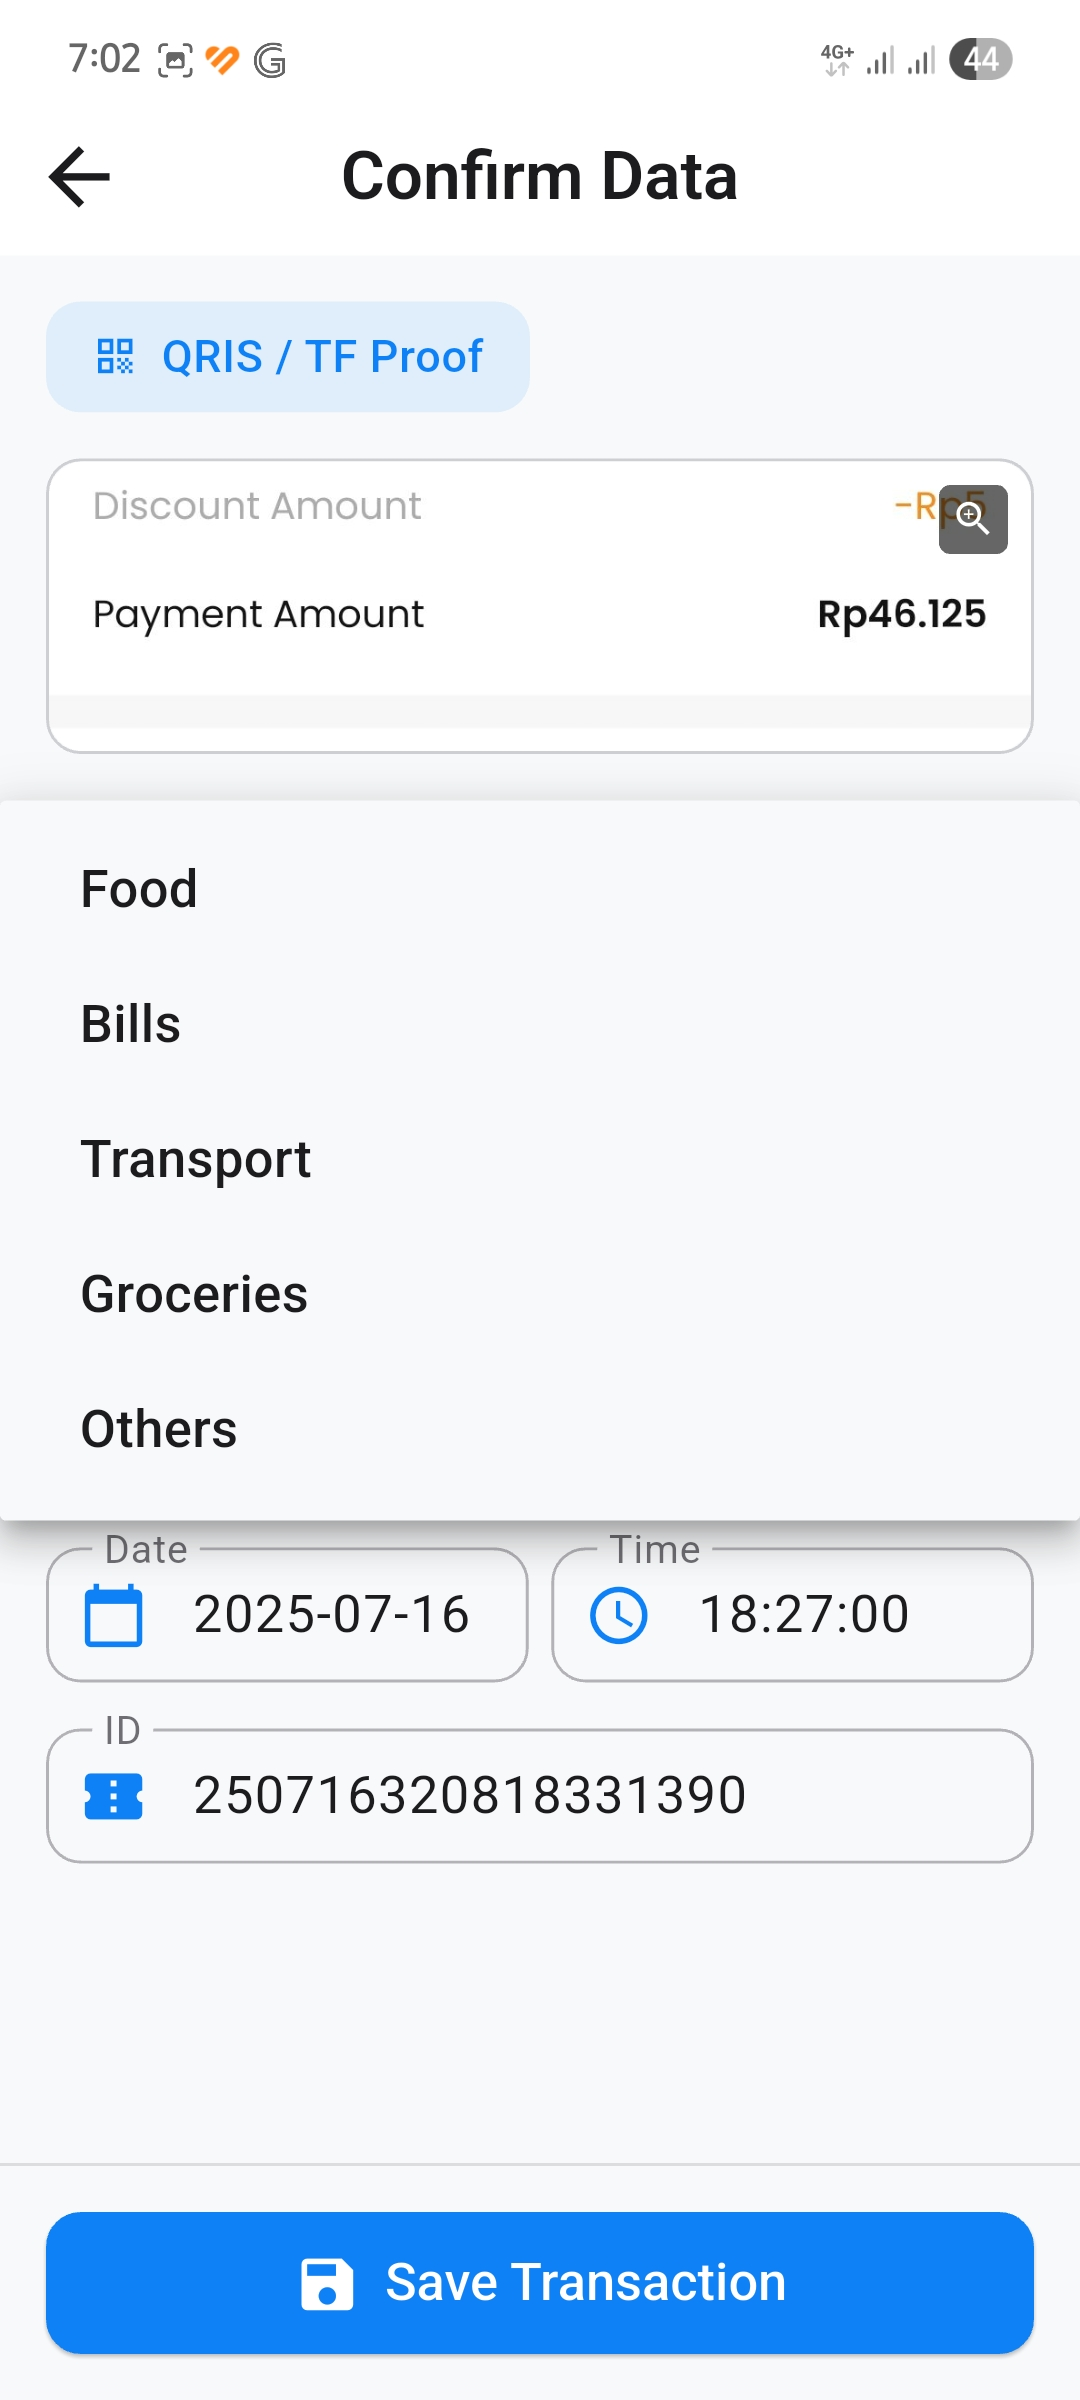
\includegraphics[width=0.33\textwidth]{images/UI/qris-cat.jpg} &
    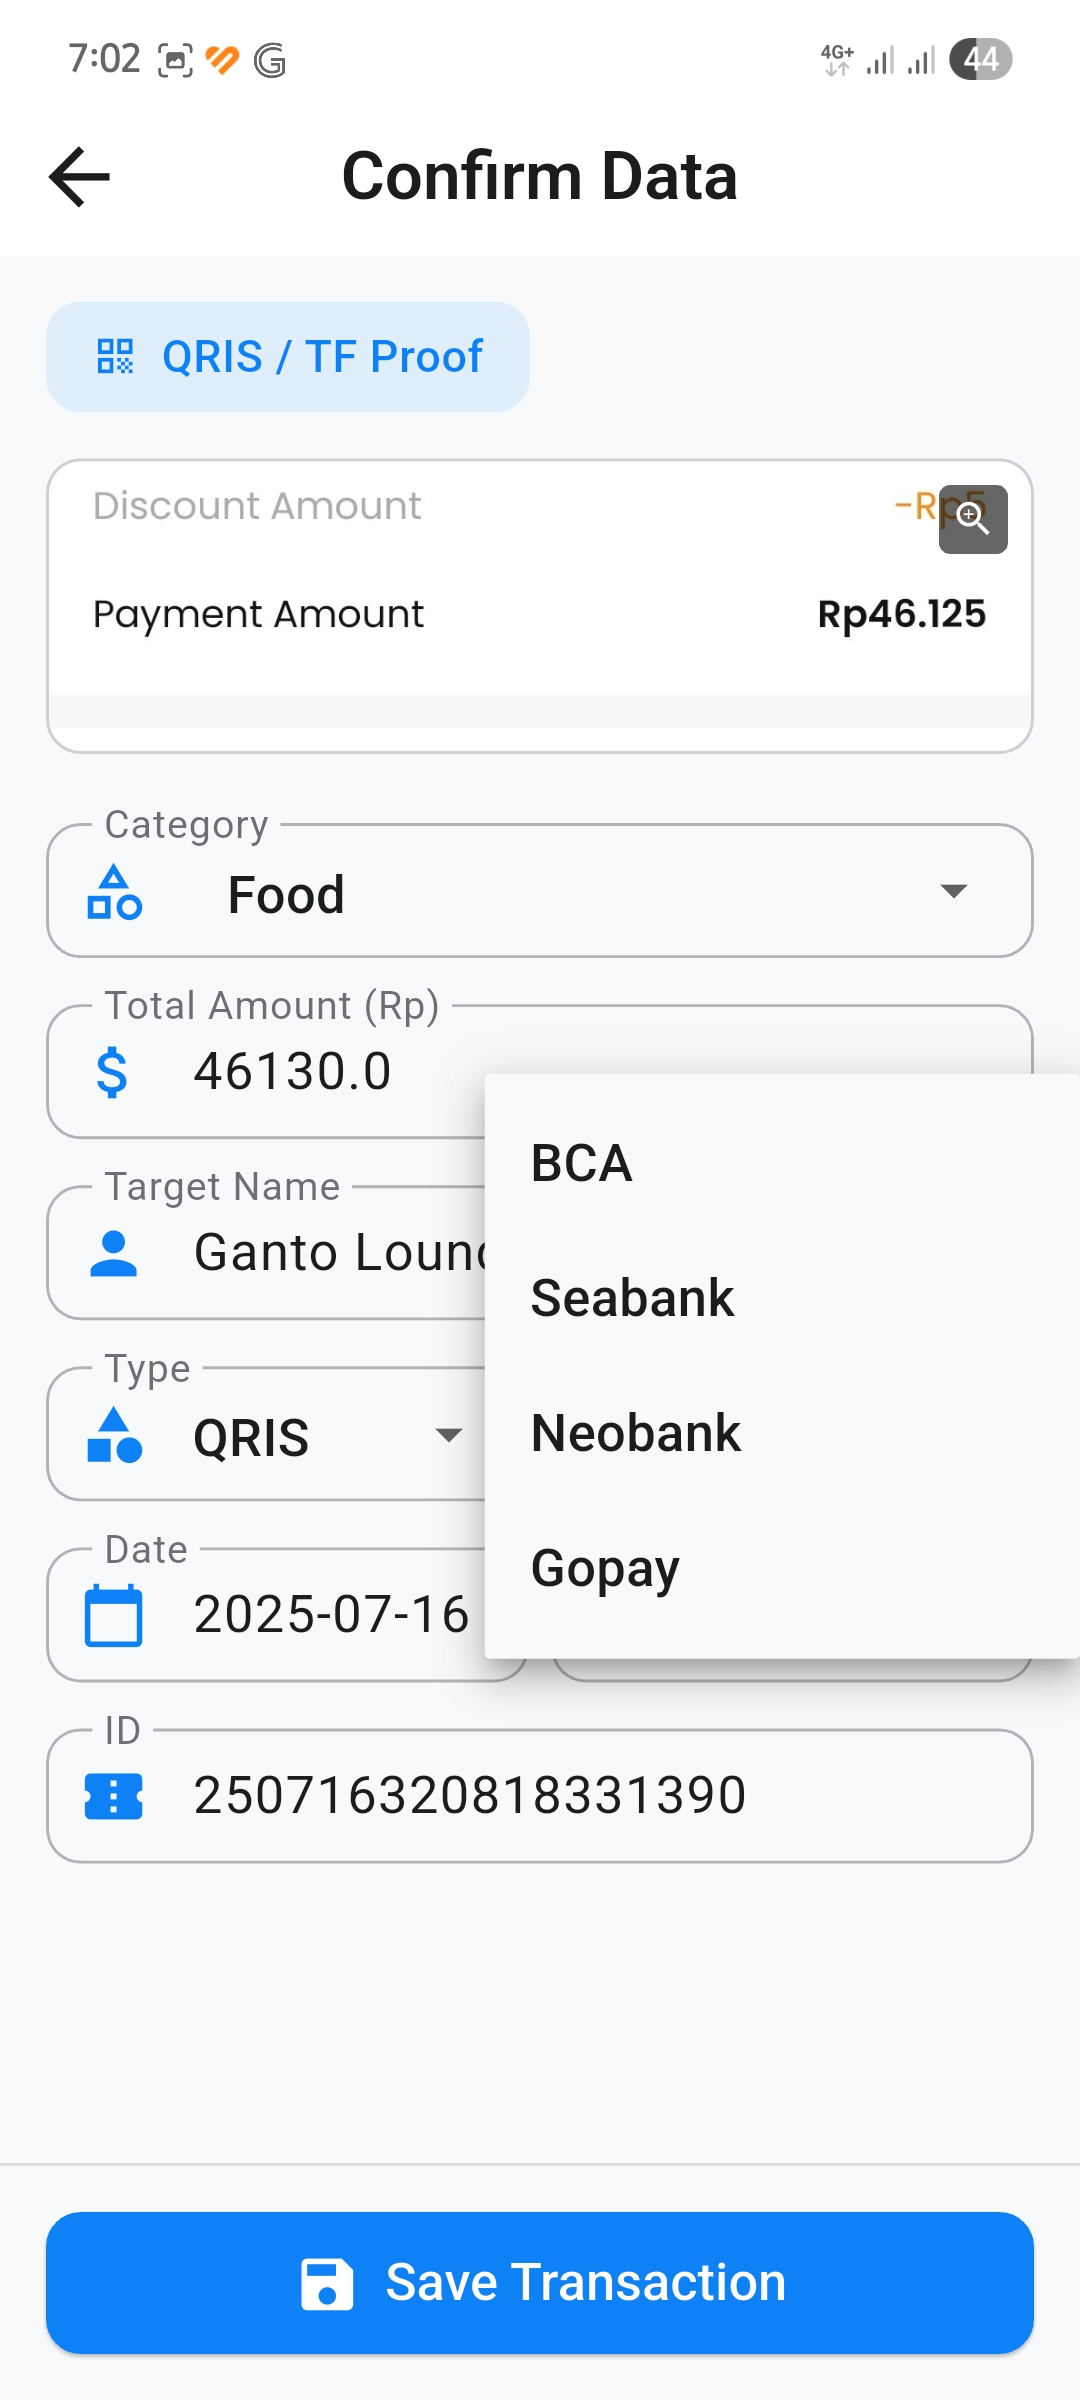
\includegraphics[width=0.33\textwidth]{images/UI/qris-a.jpg}
    \\
    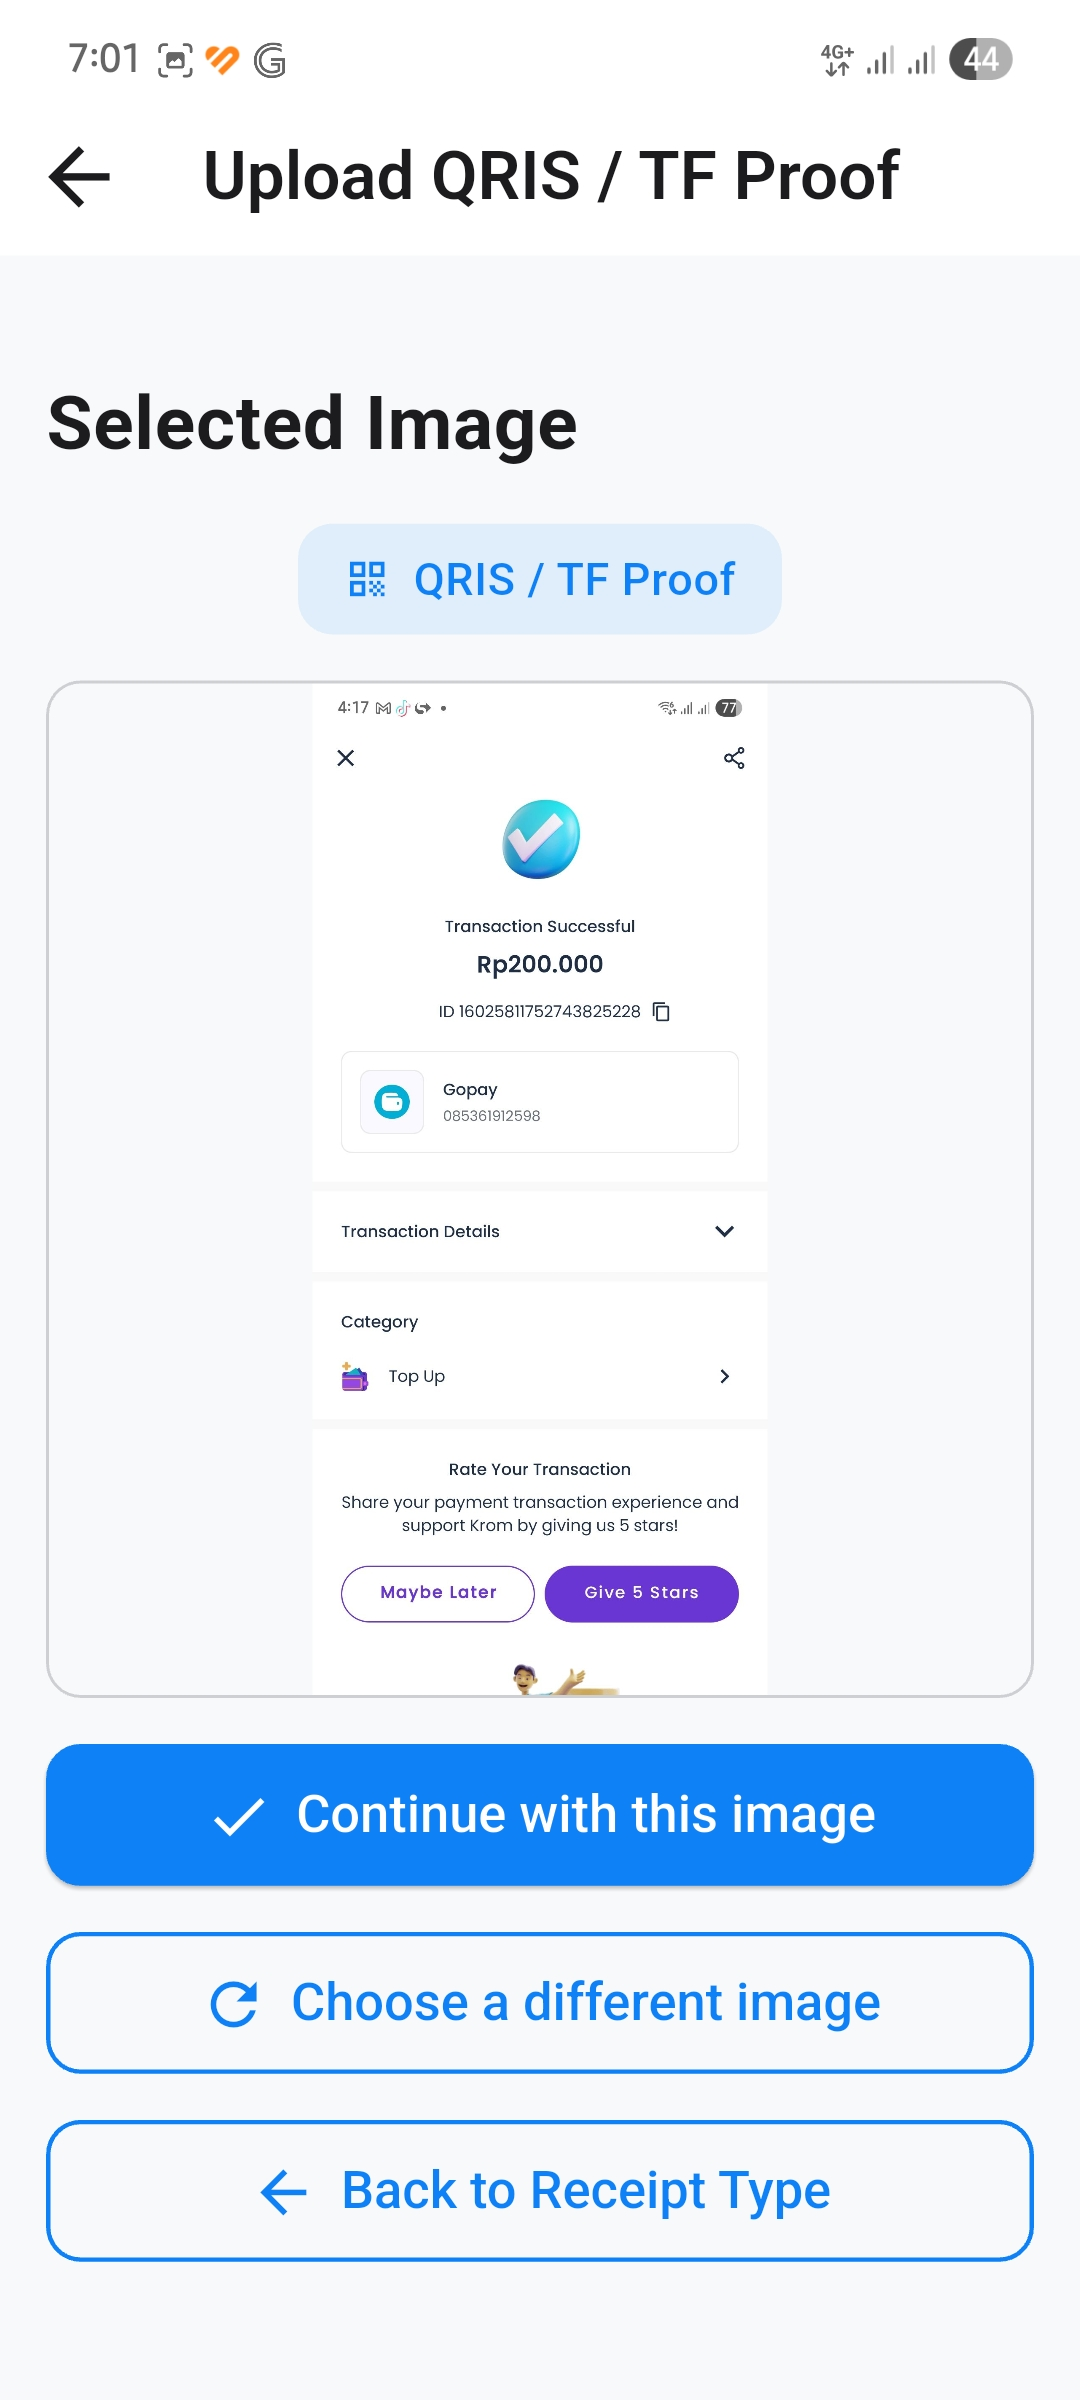
\includegraphics[width=0.33\textwidth]{images/UI/qris-confirm.jpg} &
    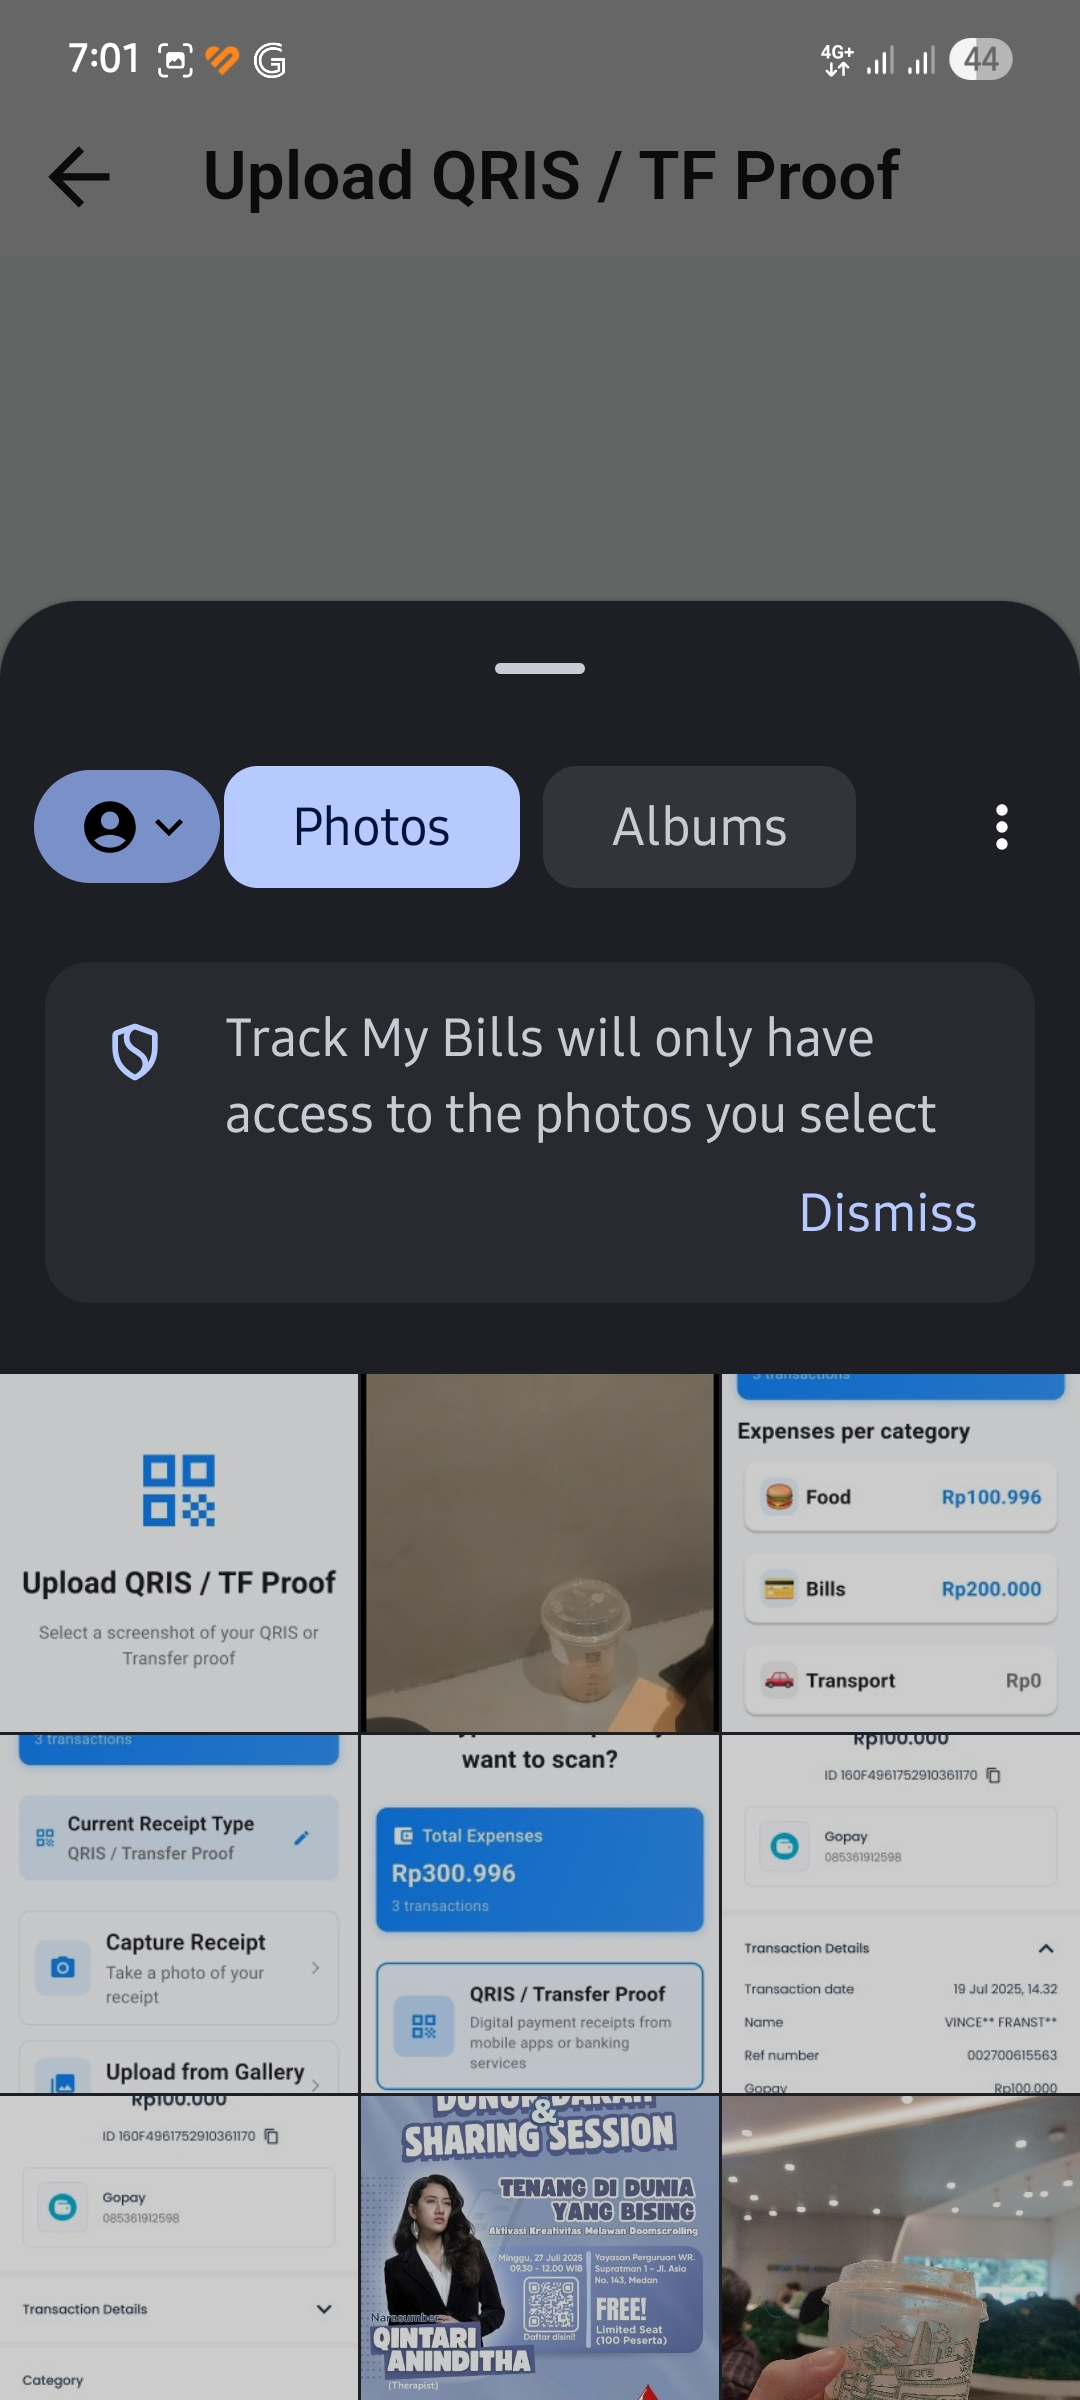
\includegraphics[width=0.33\textwidth]{images/UI/qris-galery.jpg} &
    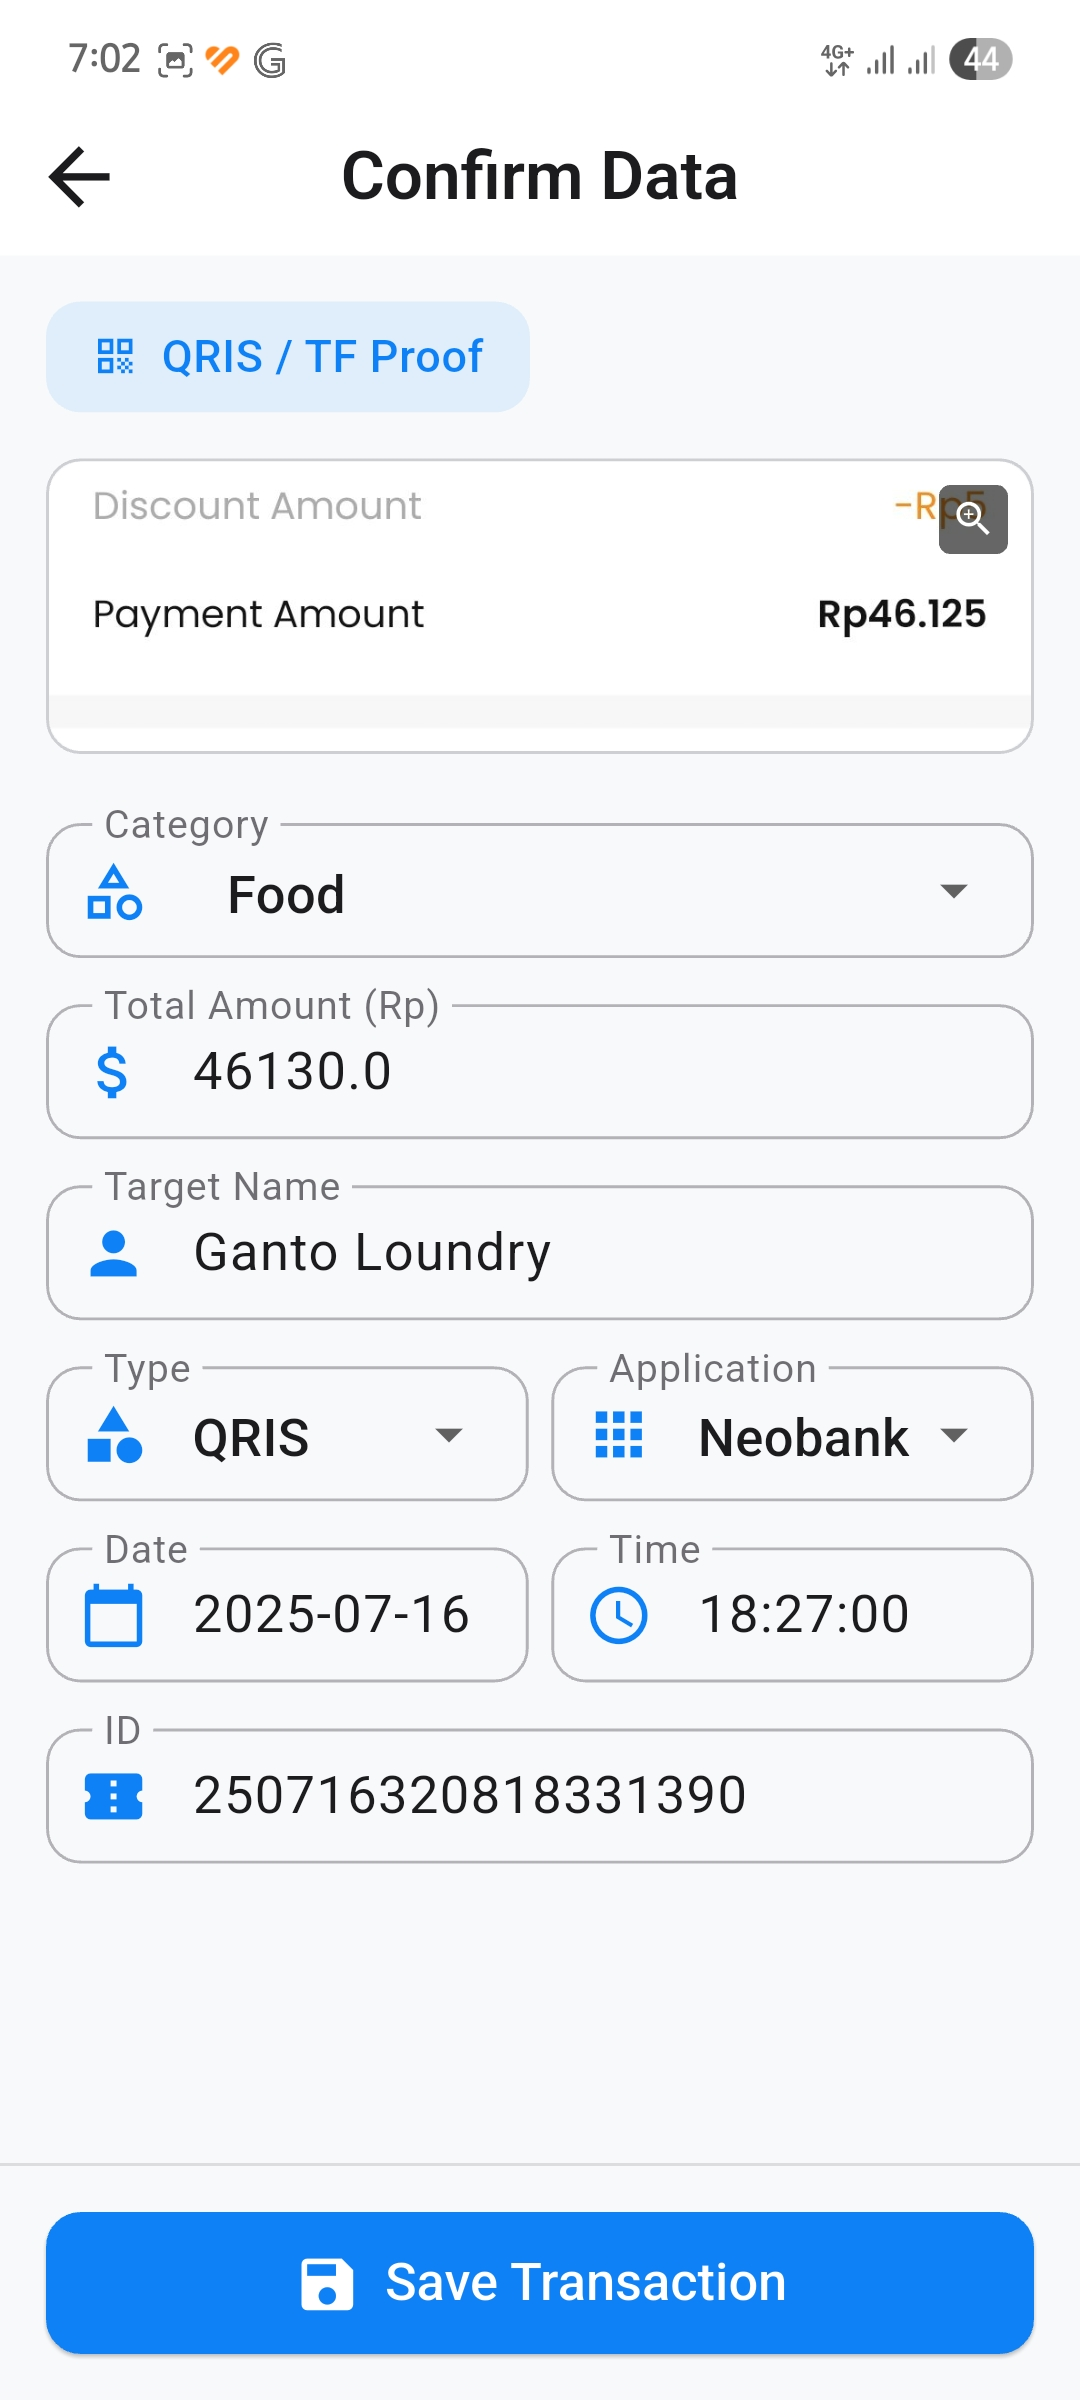
\includegraphics[width=0.33\textwidth]{images/UI/qris-mapping.jpg} \\
\end{tabular}

\begin{tabular}{lll}
    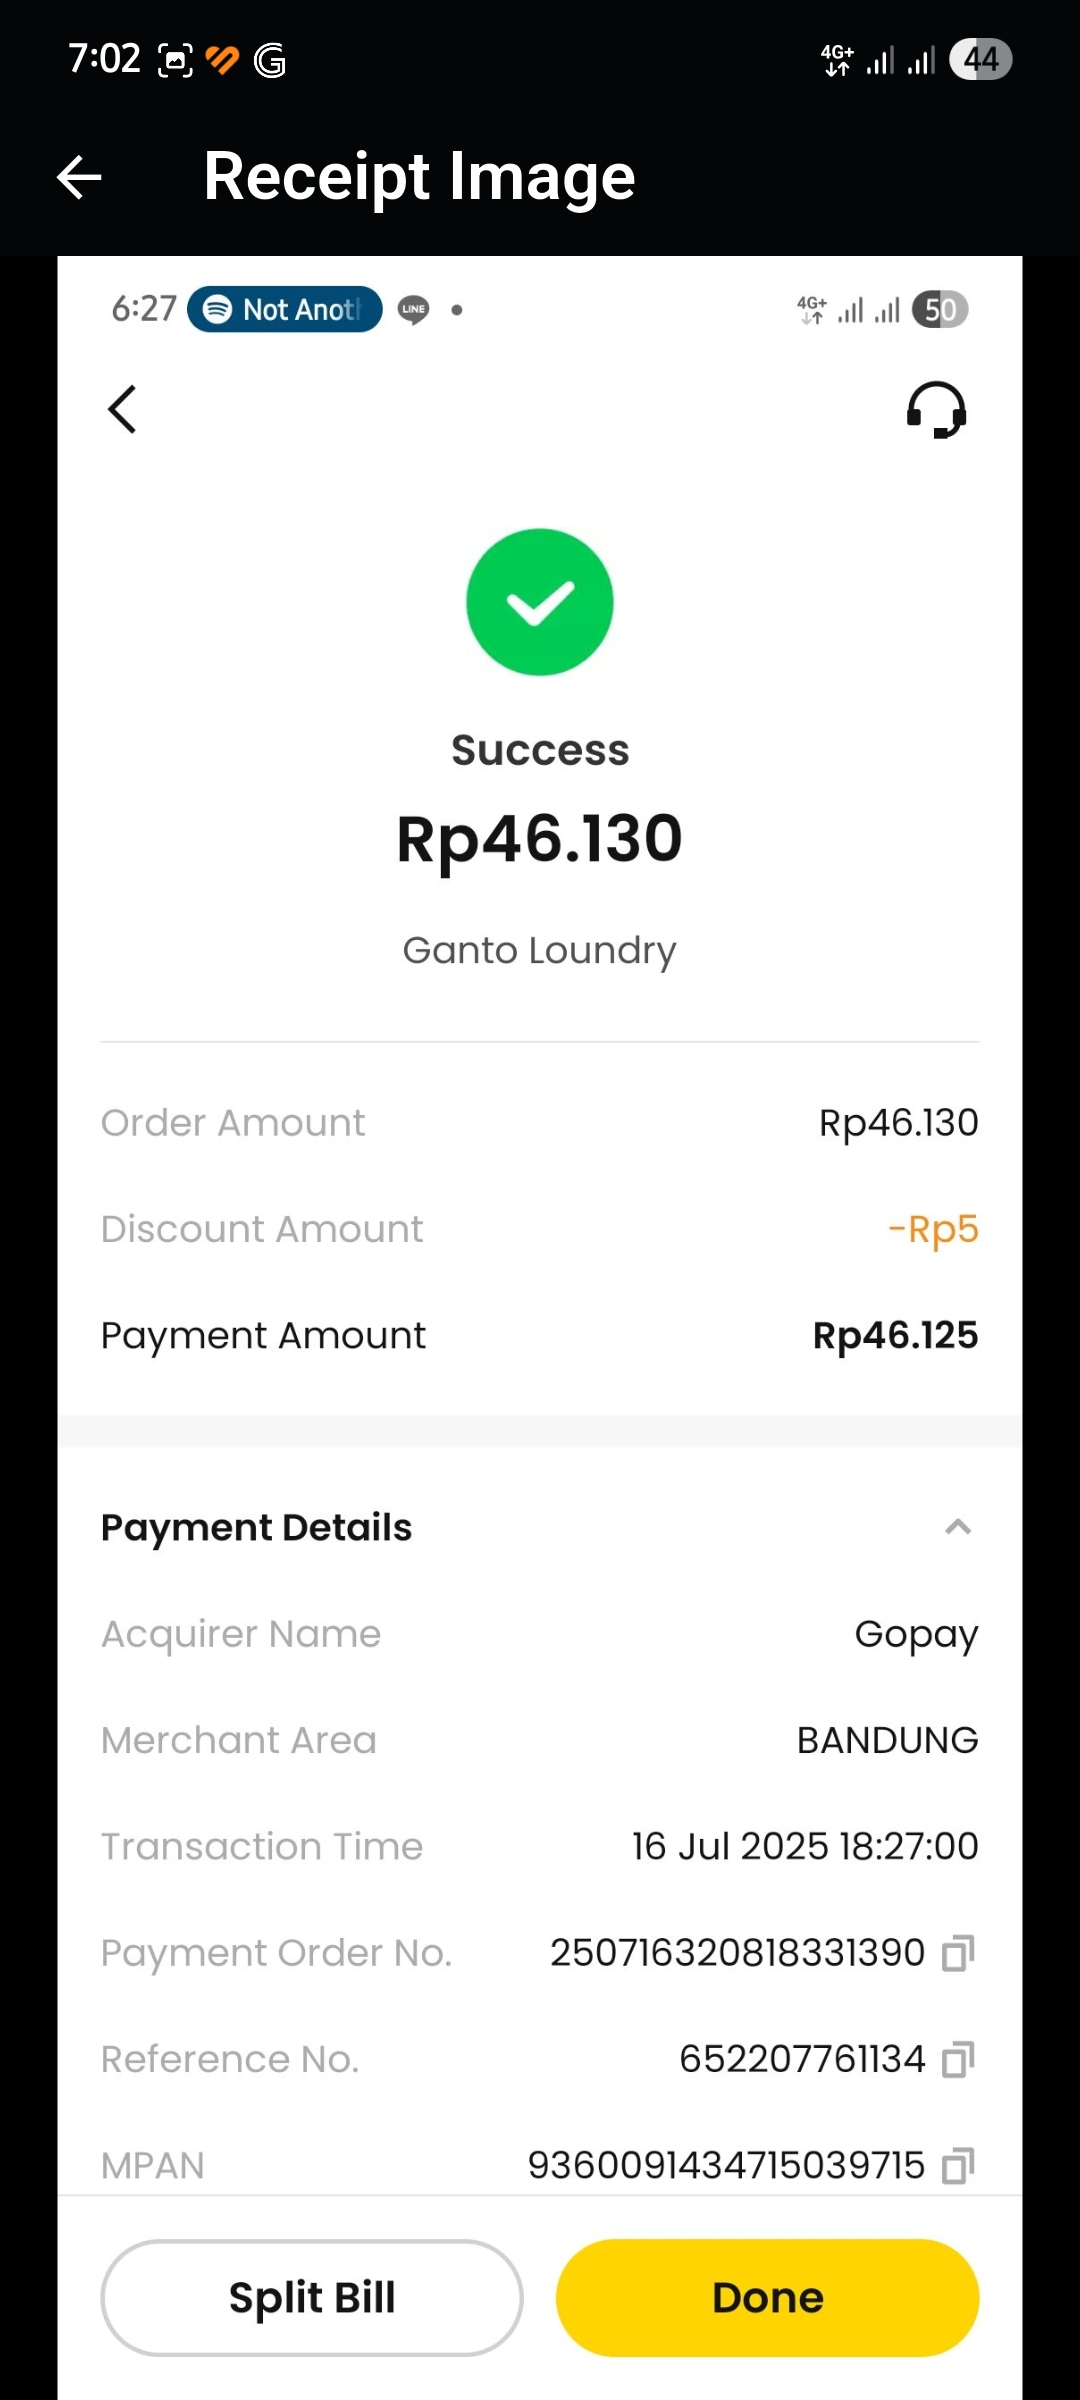
\includegraphics[width=0.33\textwidth]{images/UI/qris-recheck.jpg} &
    
\includegraphics[width=0.33\textwidth]{images/UI/qris-review.jpg} &
    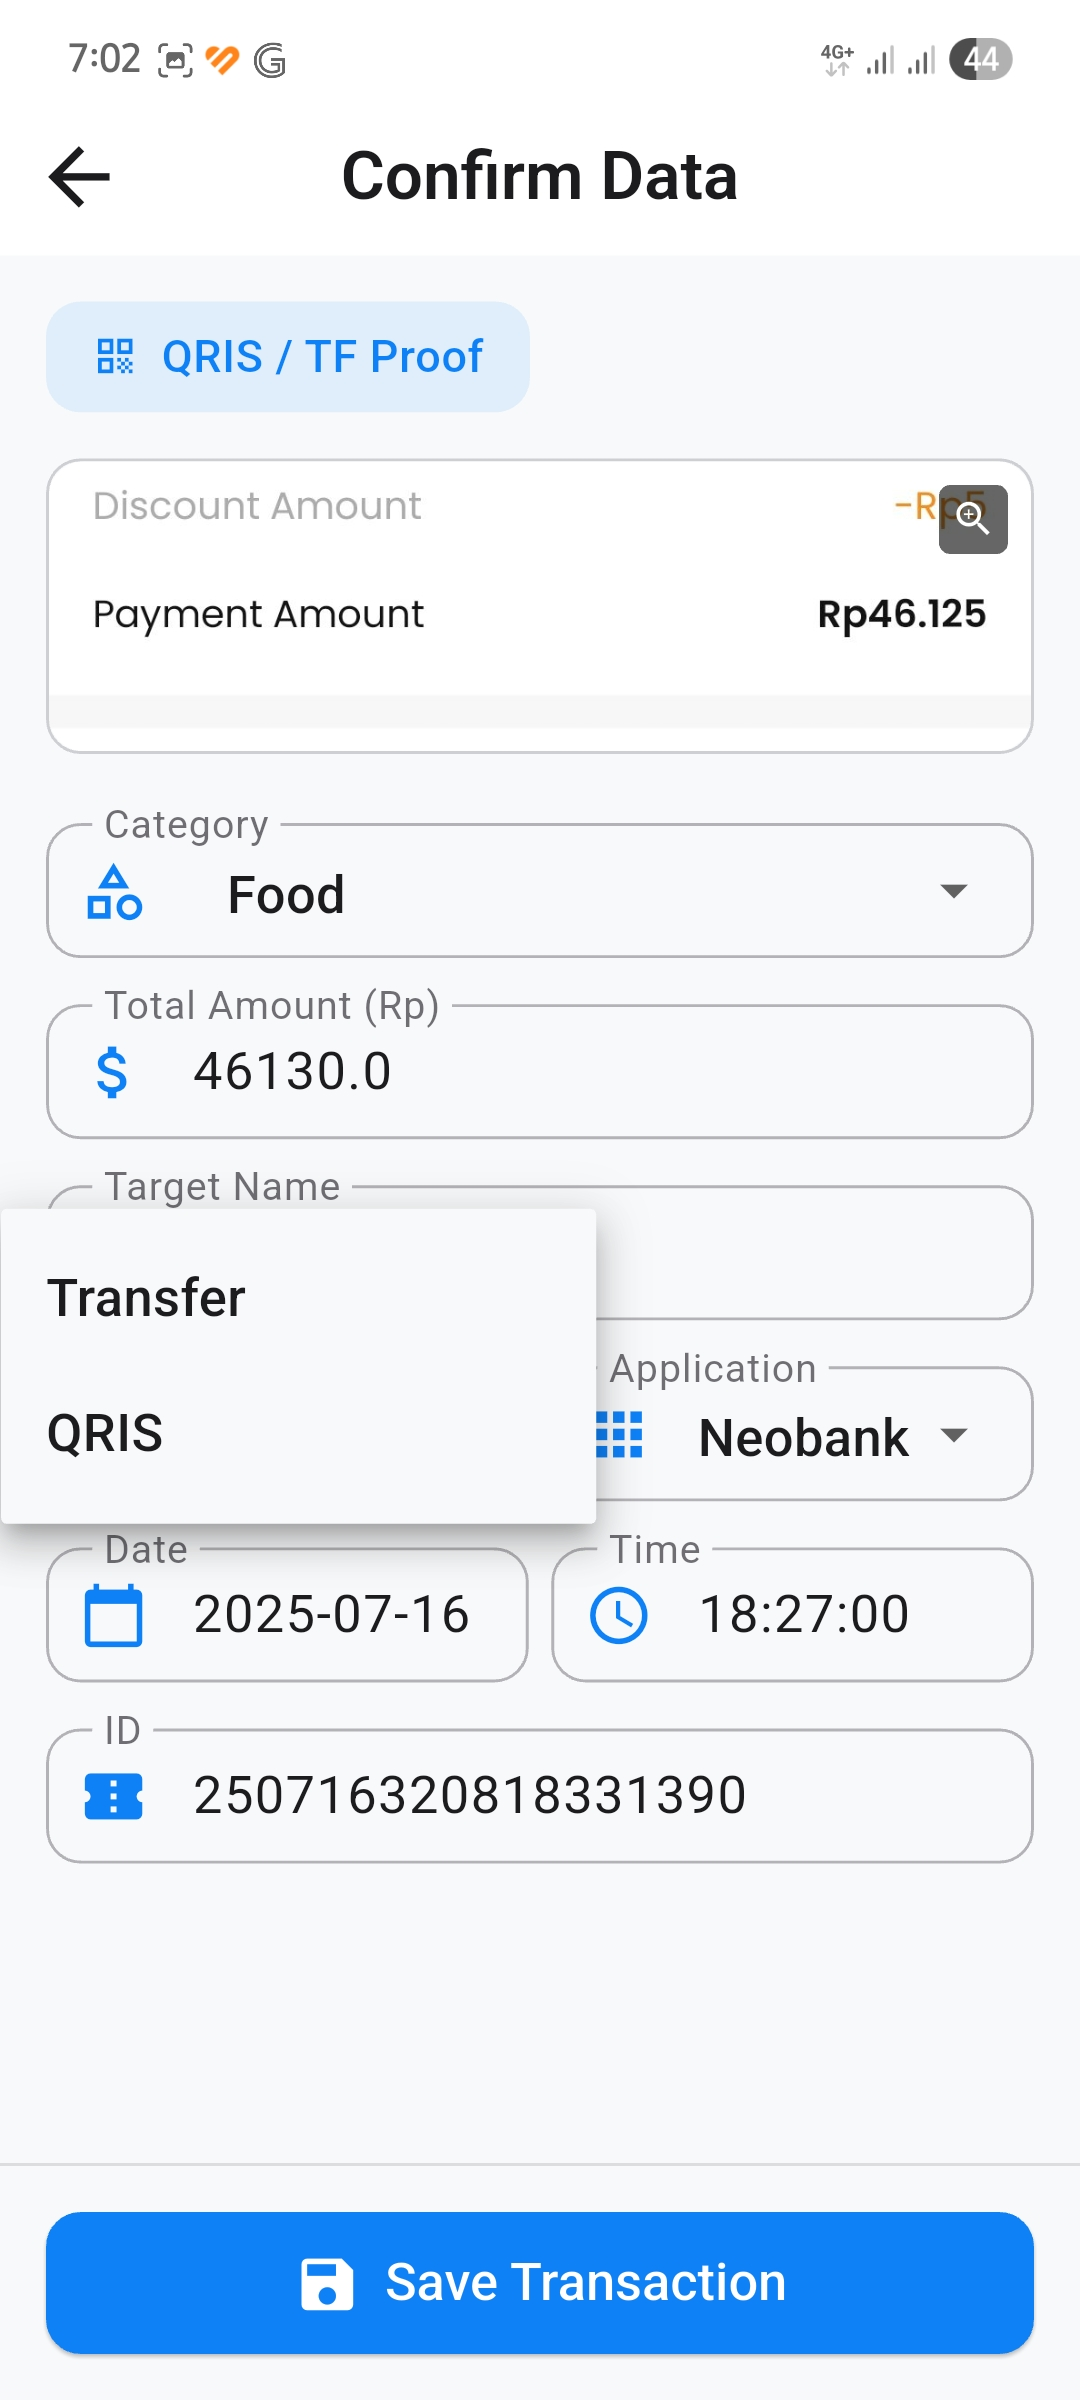
\includegraphics[width=0.33\textwidth]{images/UI/qris-t.jpg}
    \\
    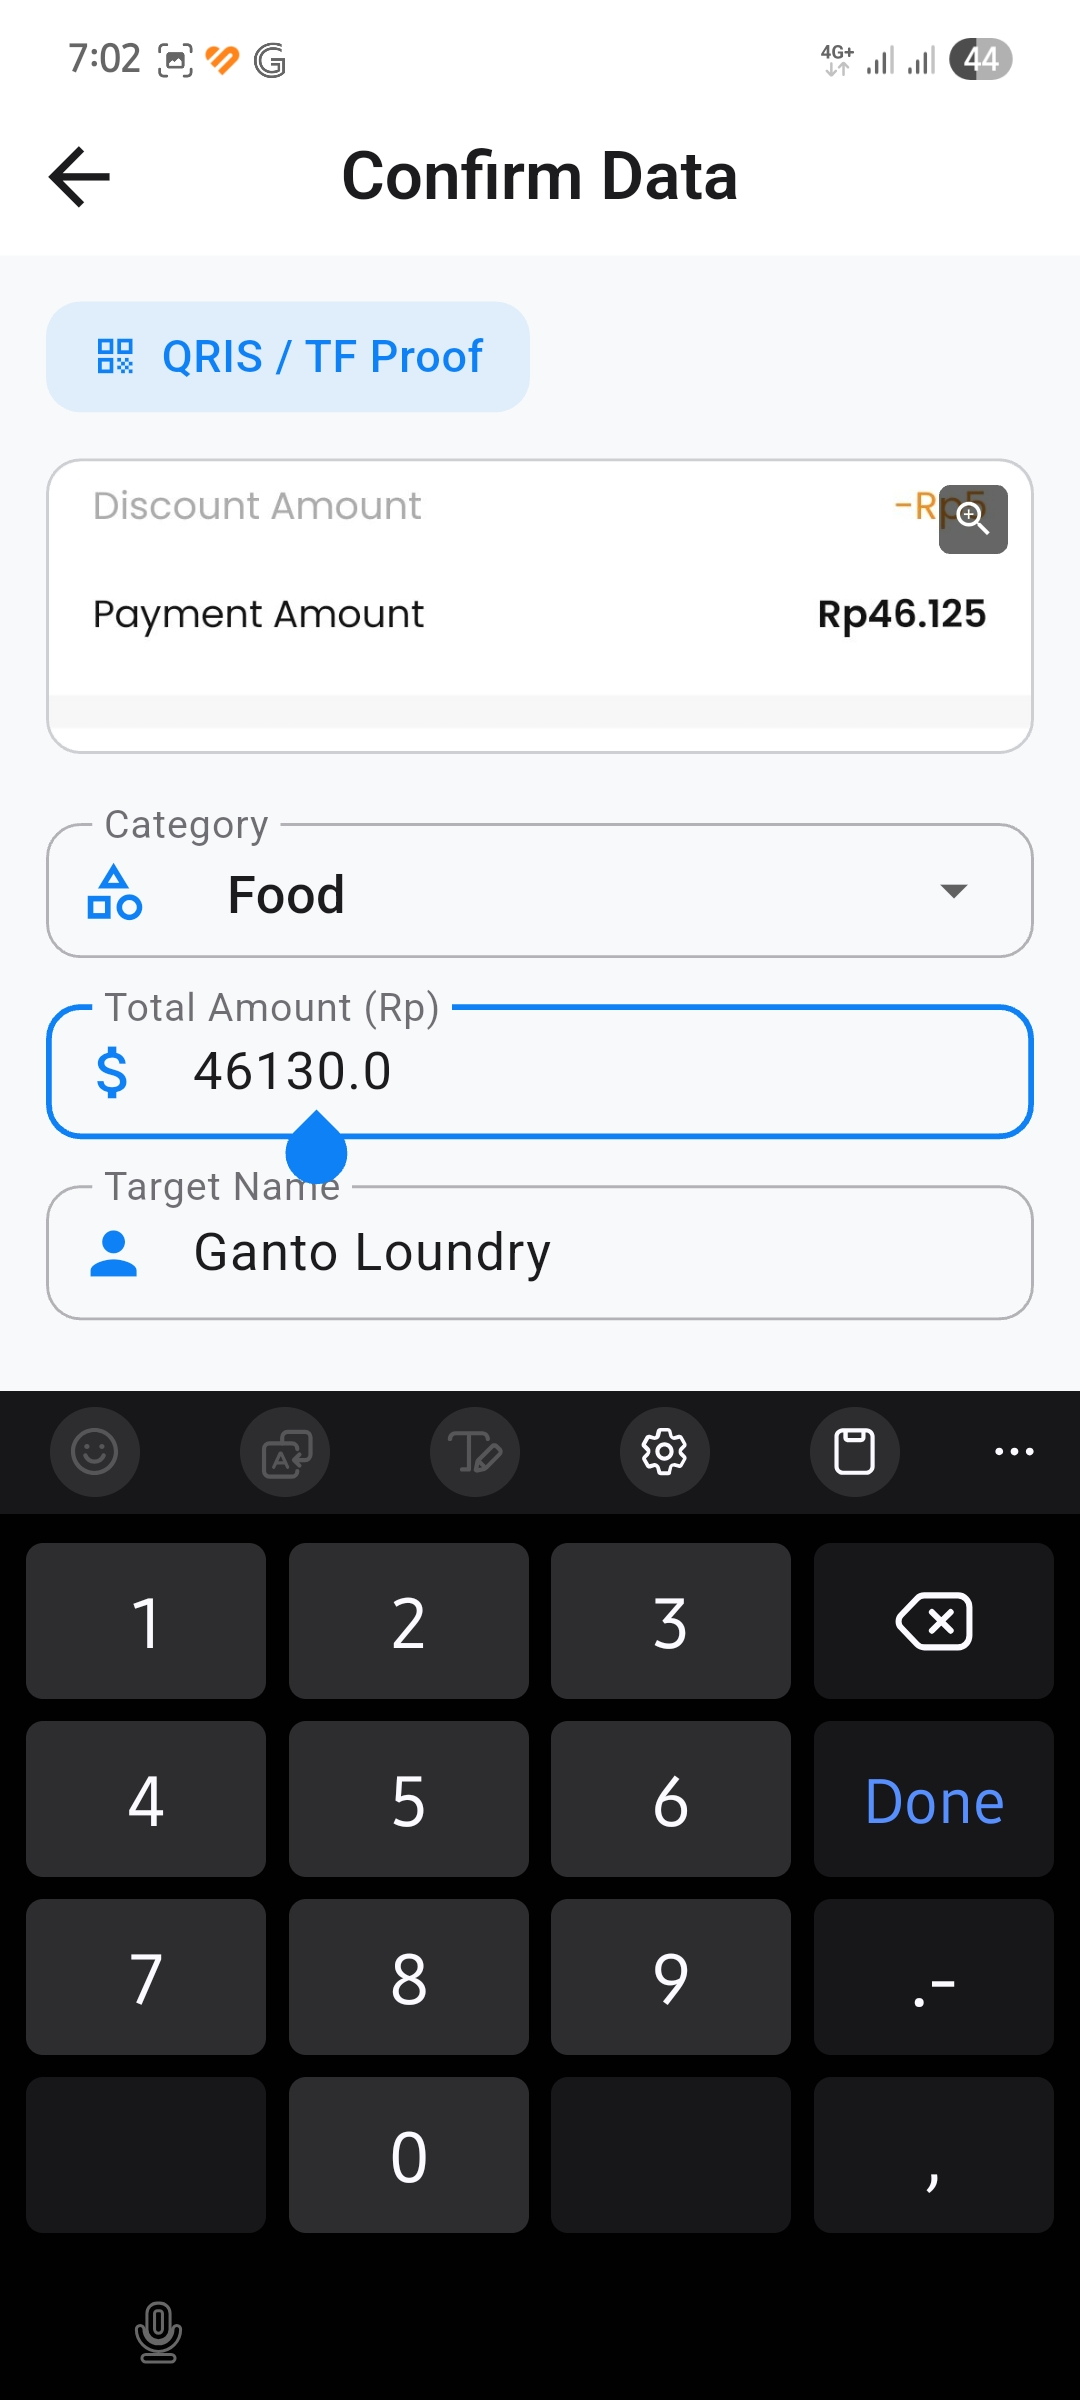
\includegraphics[width=0.33\textwidth]{images/UI/qris-ta.jpg} &
    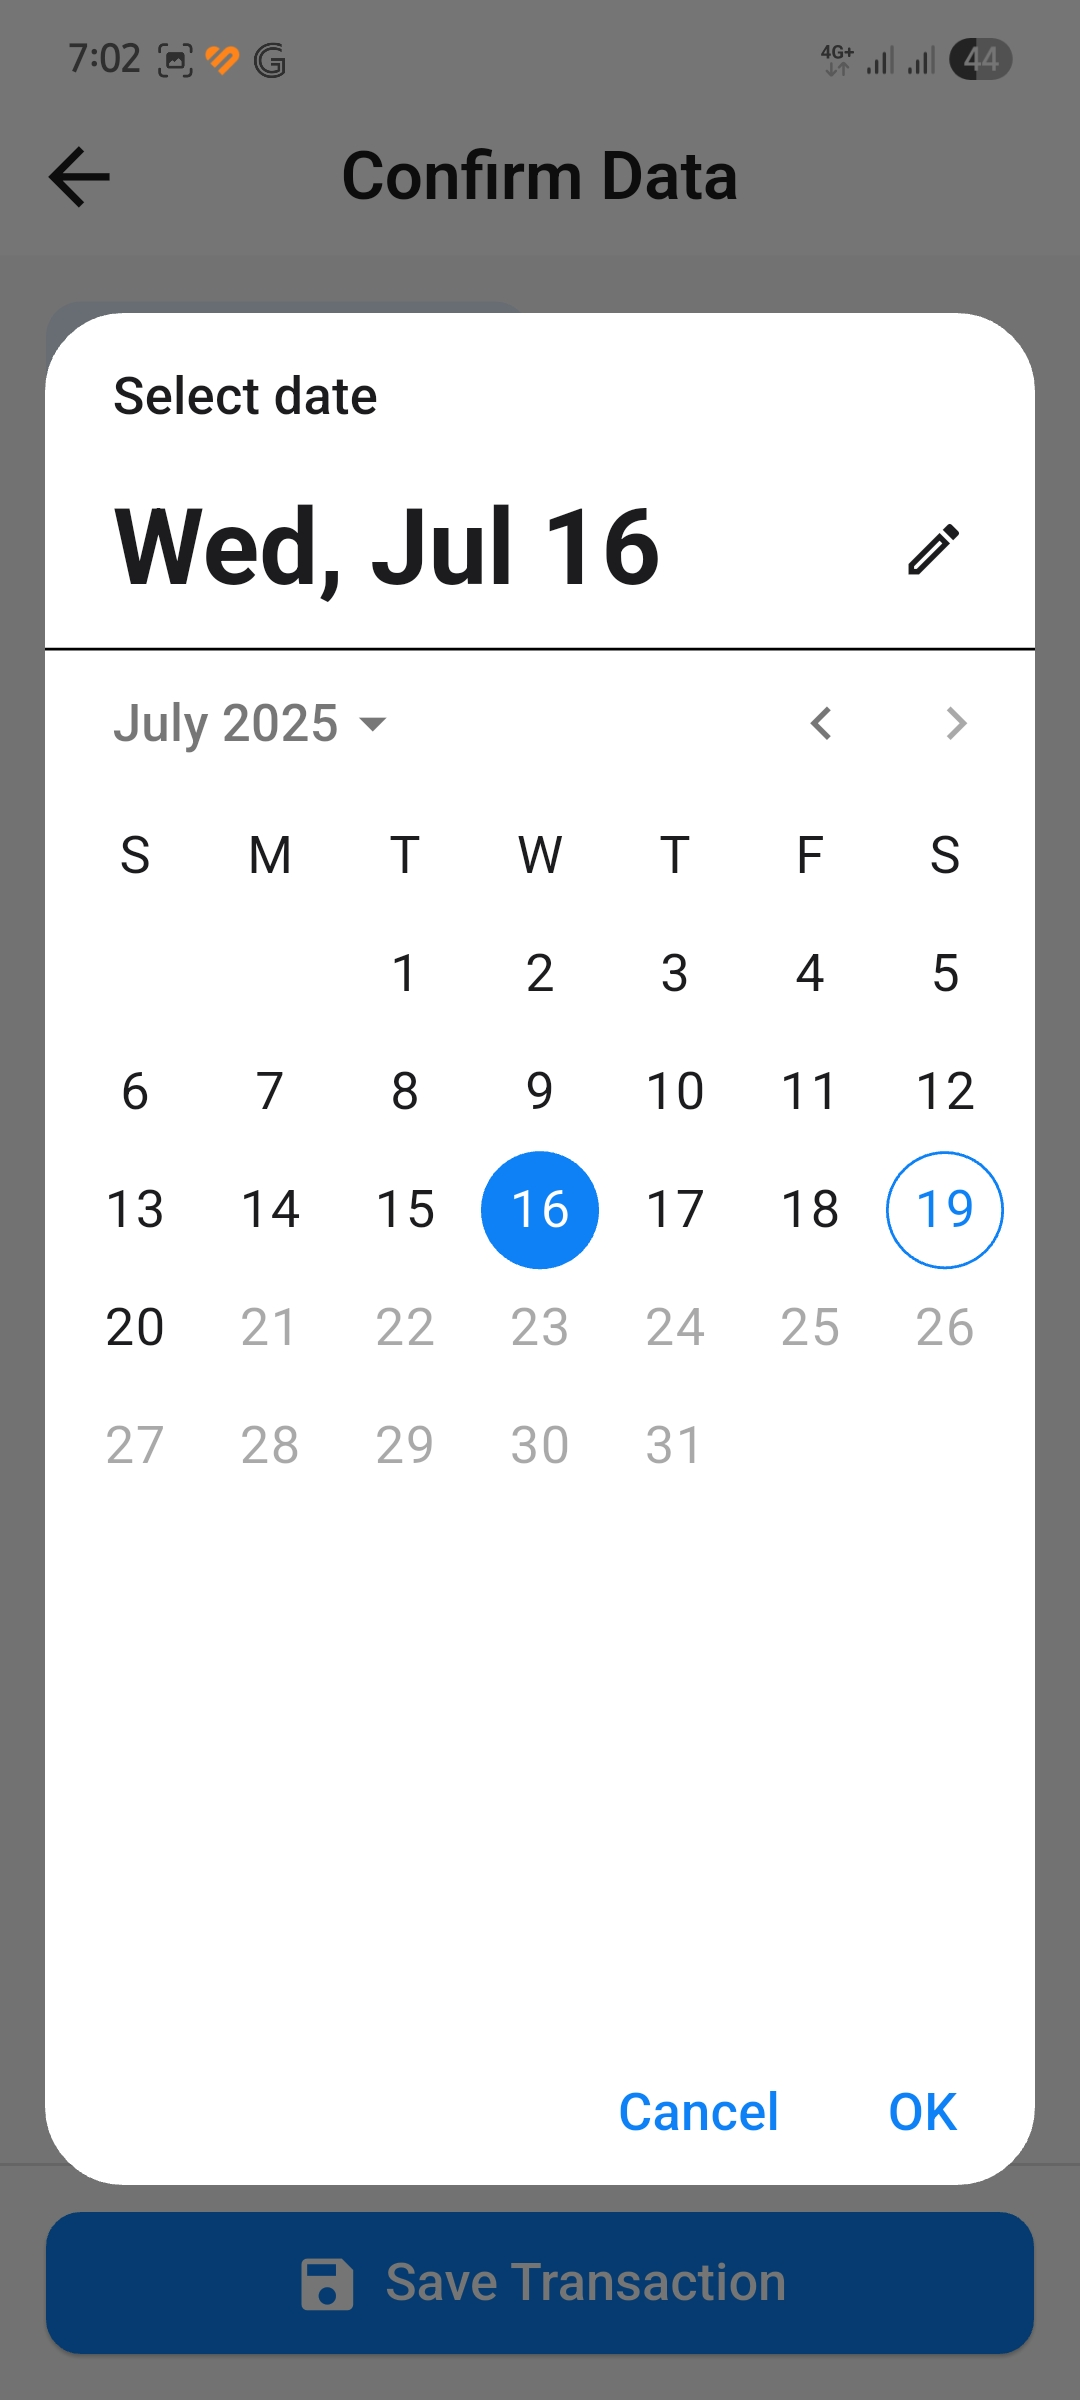
\includegraphics[width=0.33\textwidth]{images/UI/qris-td.jpg} &
    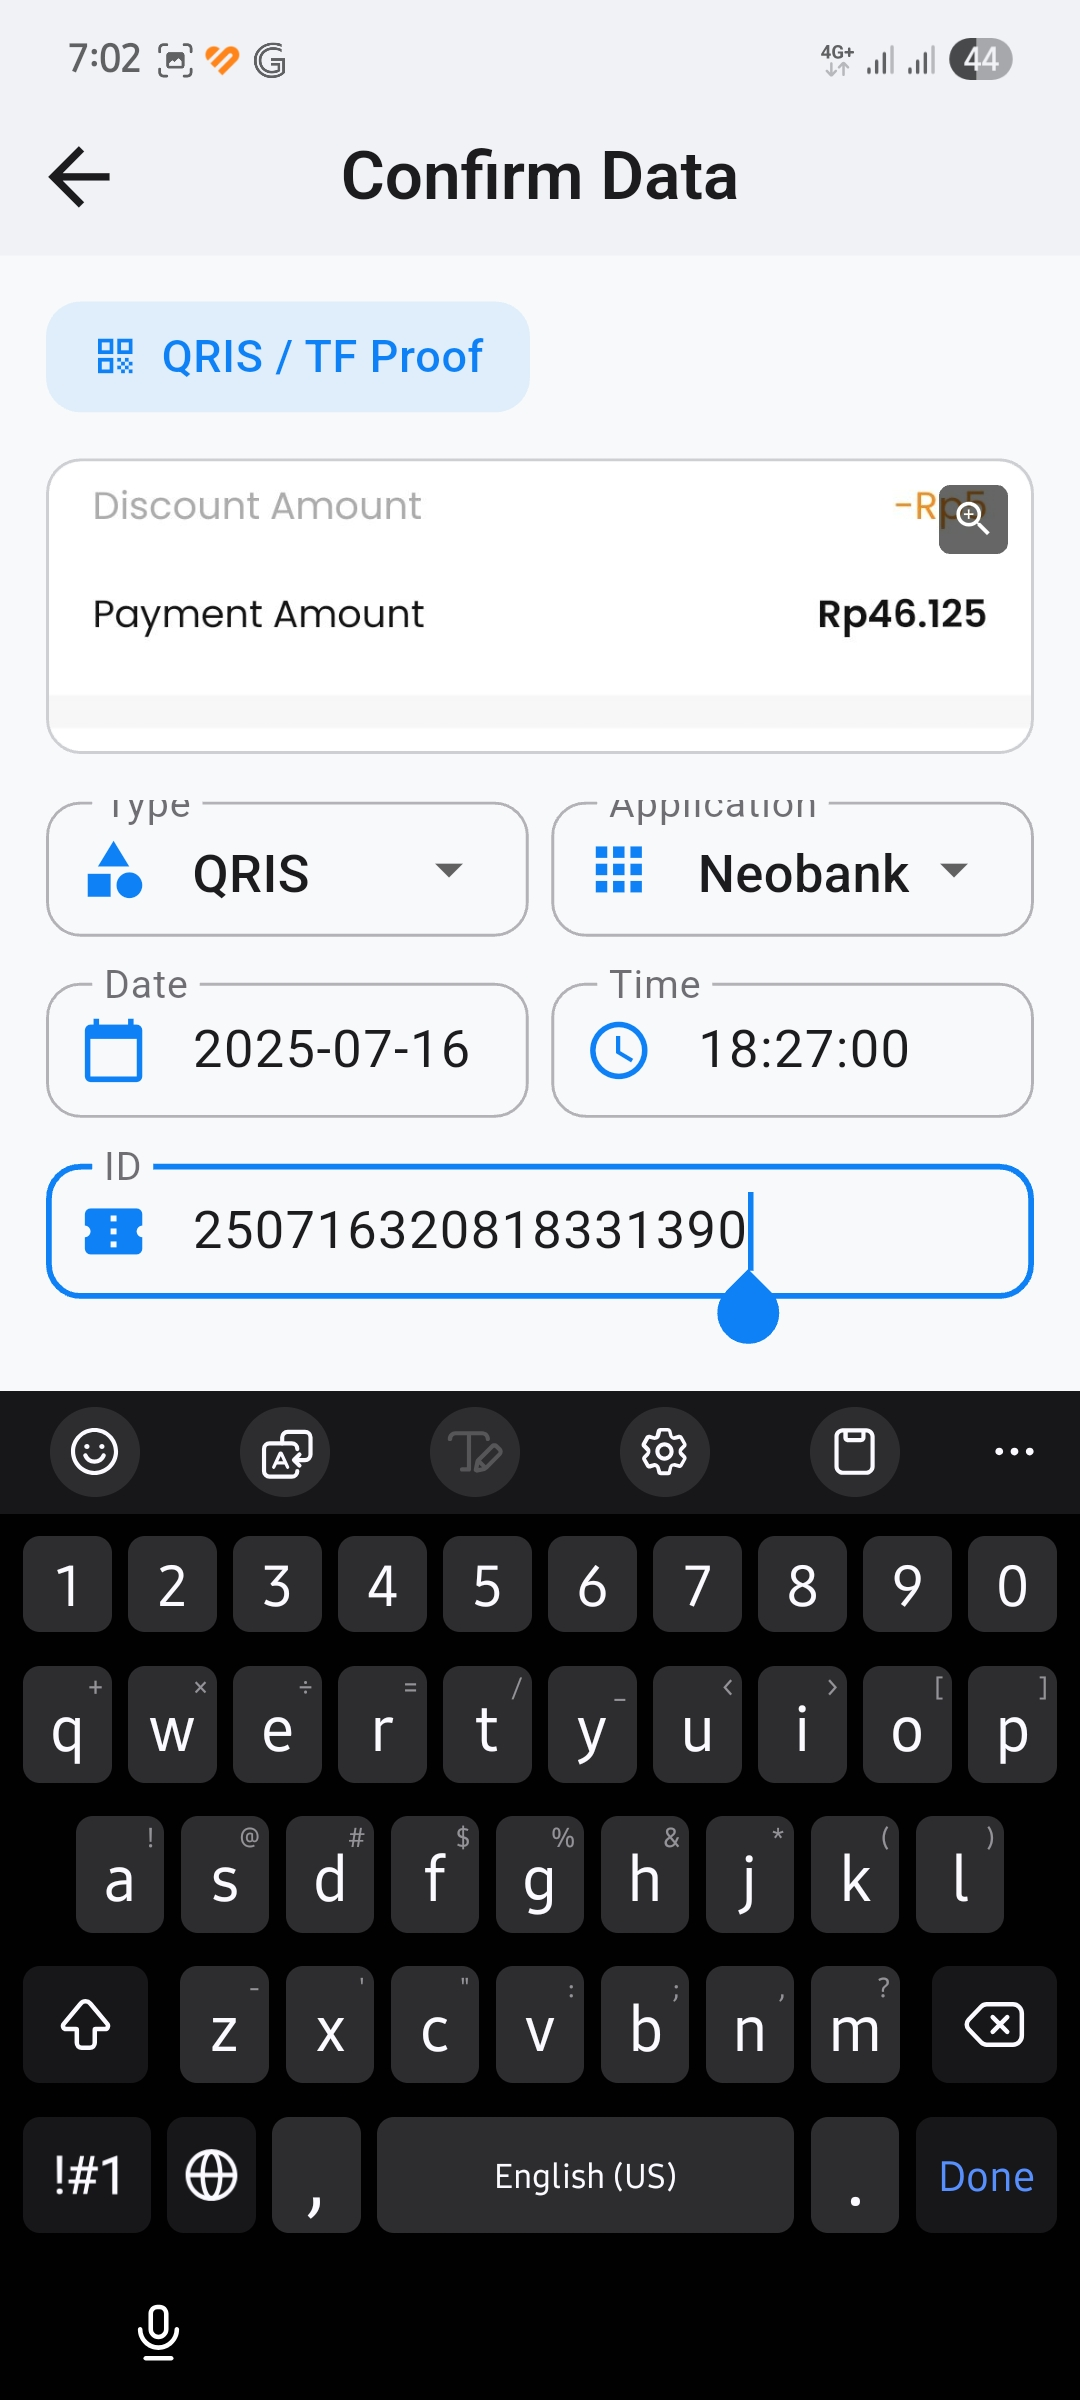
\includegraphics[width=0.33\textwidth]{images/UI/qris-tid.jpg} \\
\end{tabular}

\begin{tabular}{lll}
    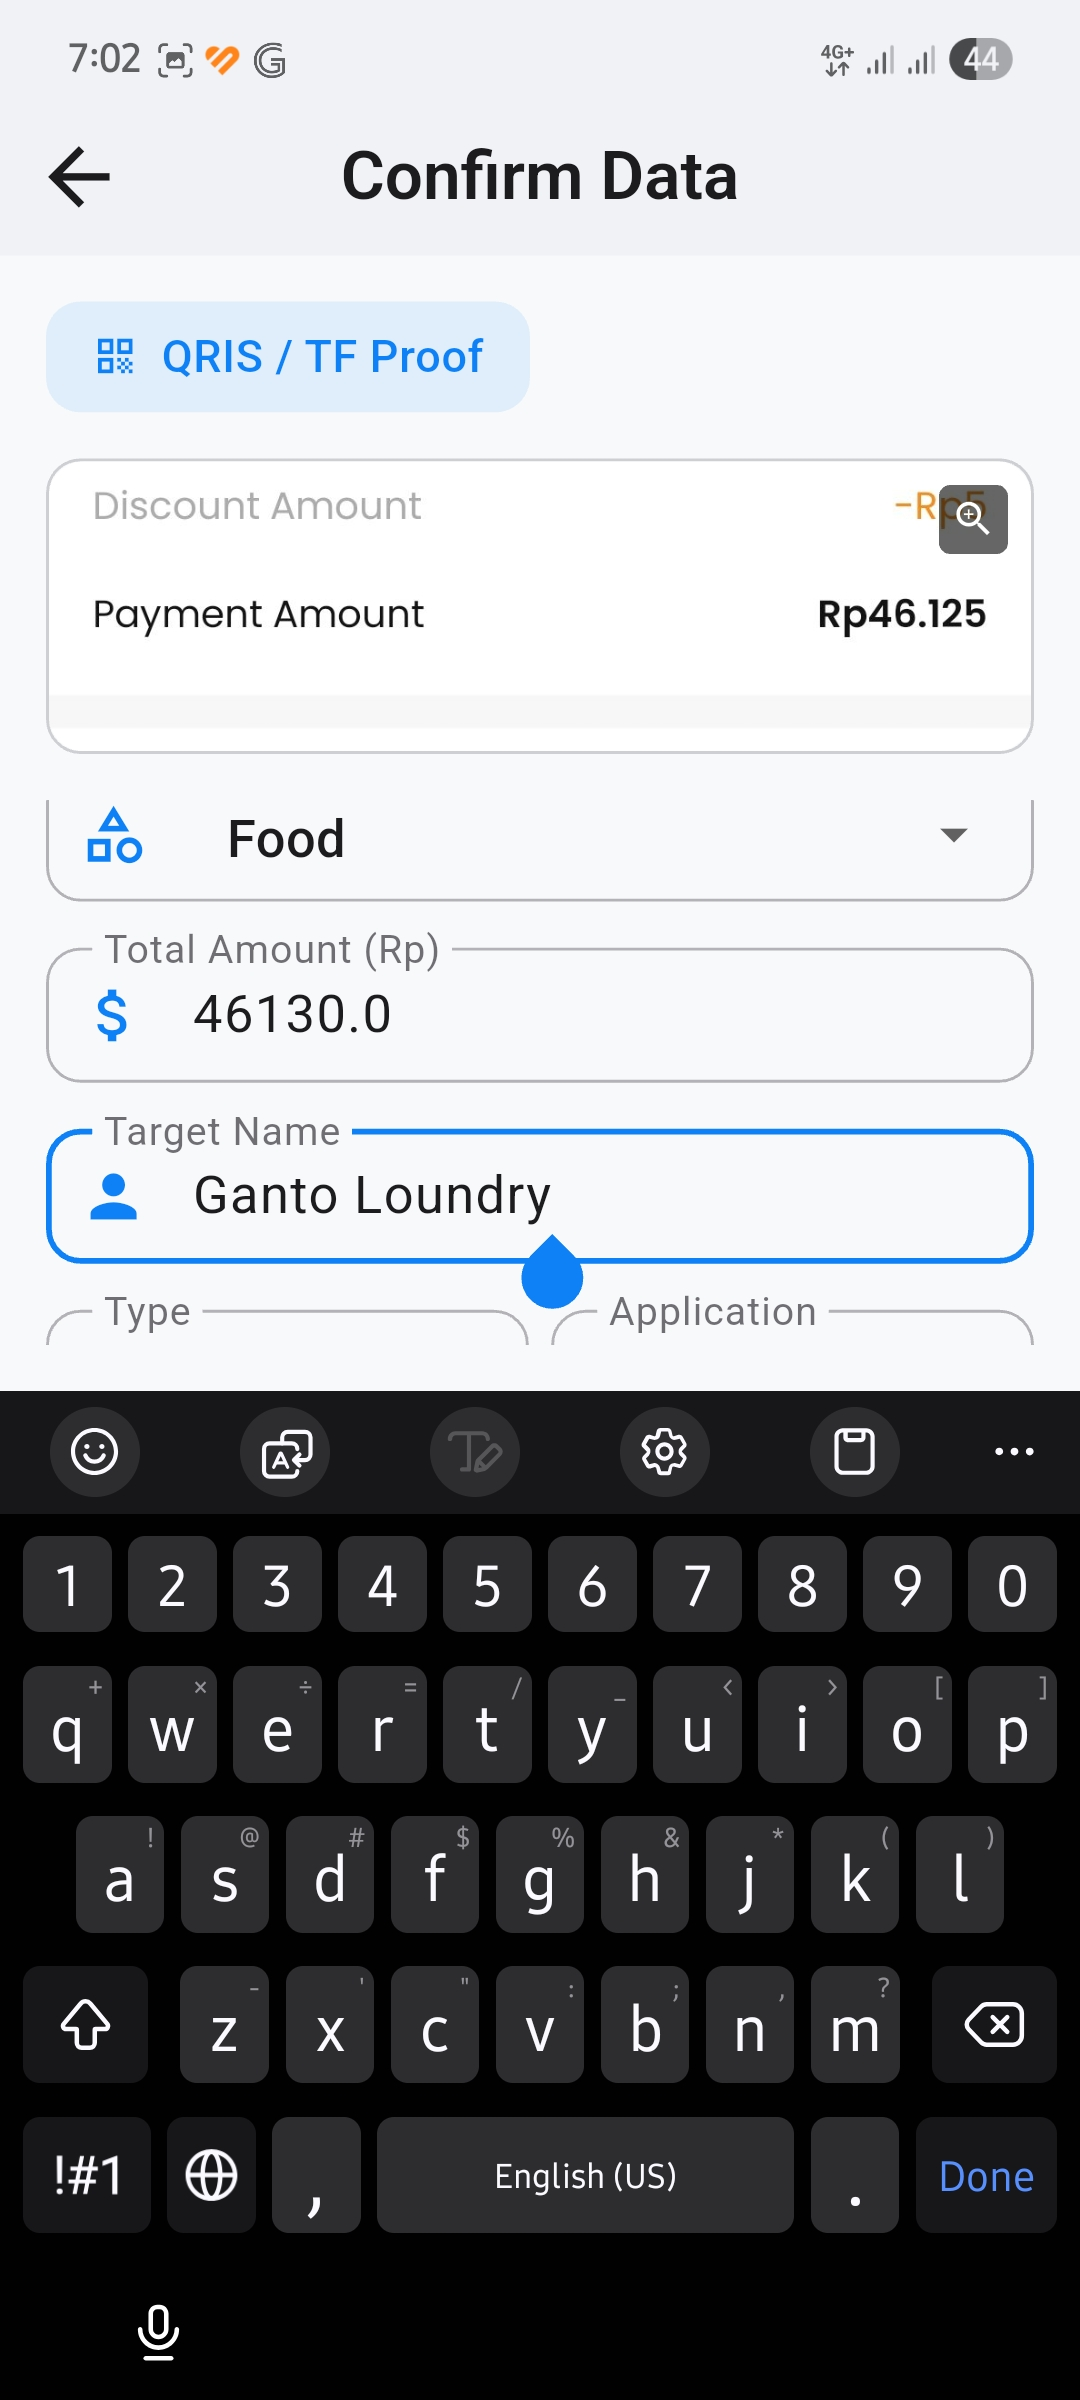
\includegraphics[width=0.33\textwidth]{images/UI/qris-tn.jpg} &
    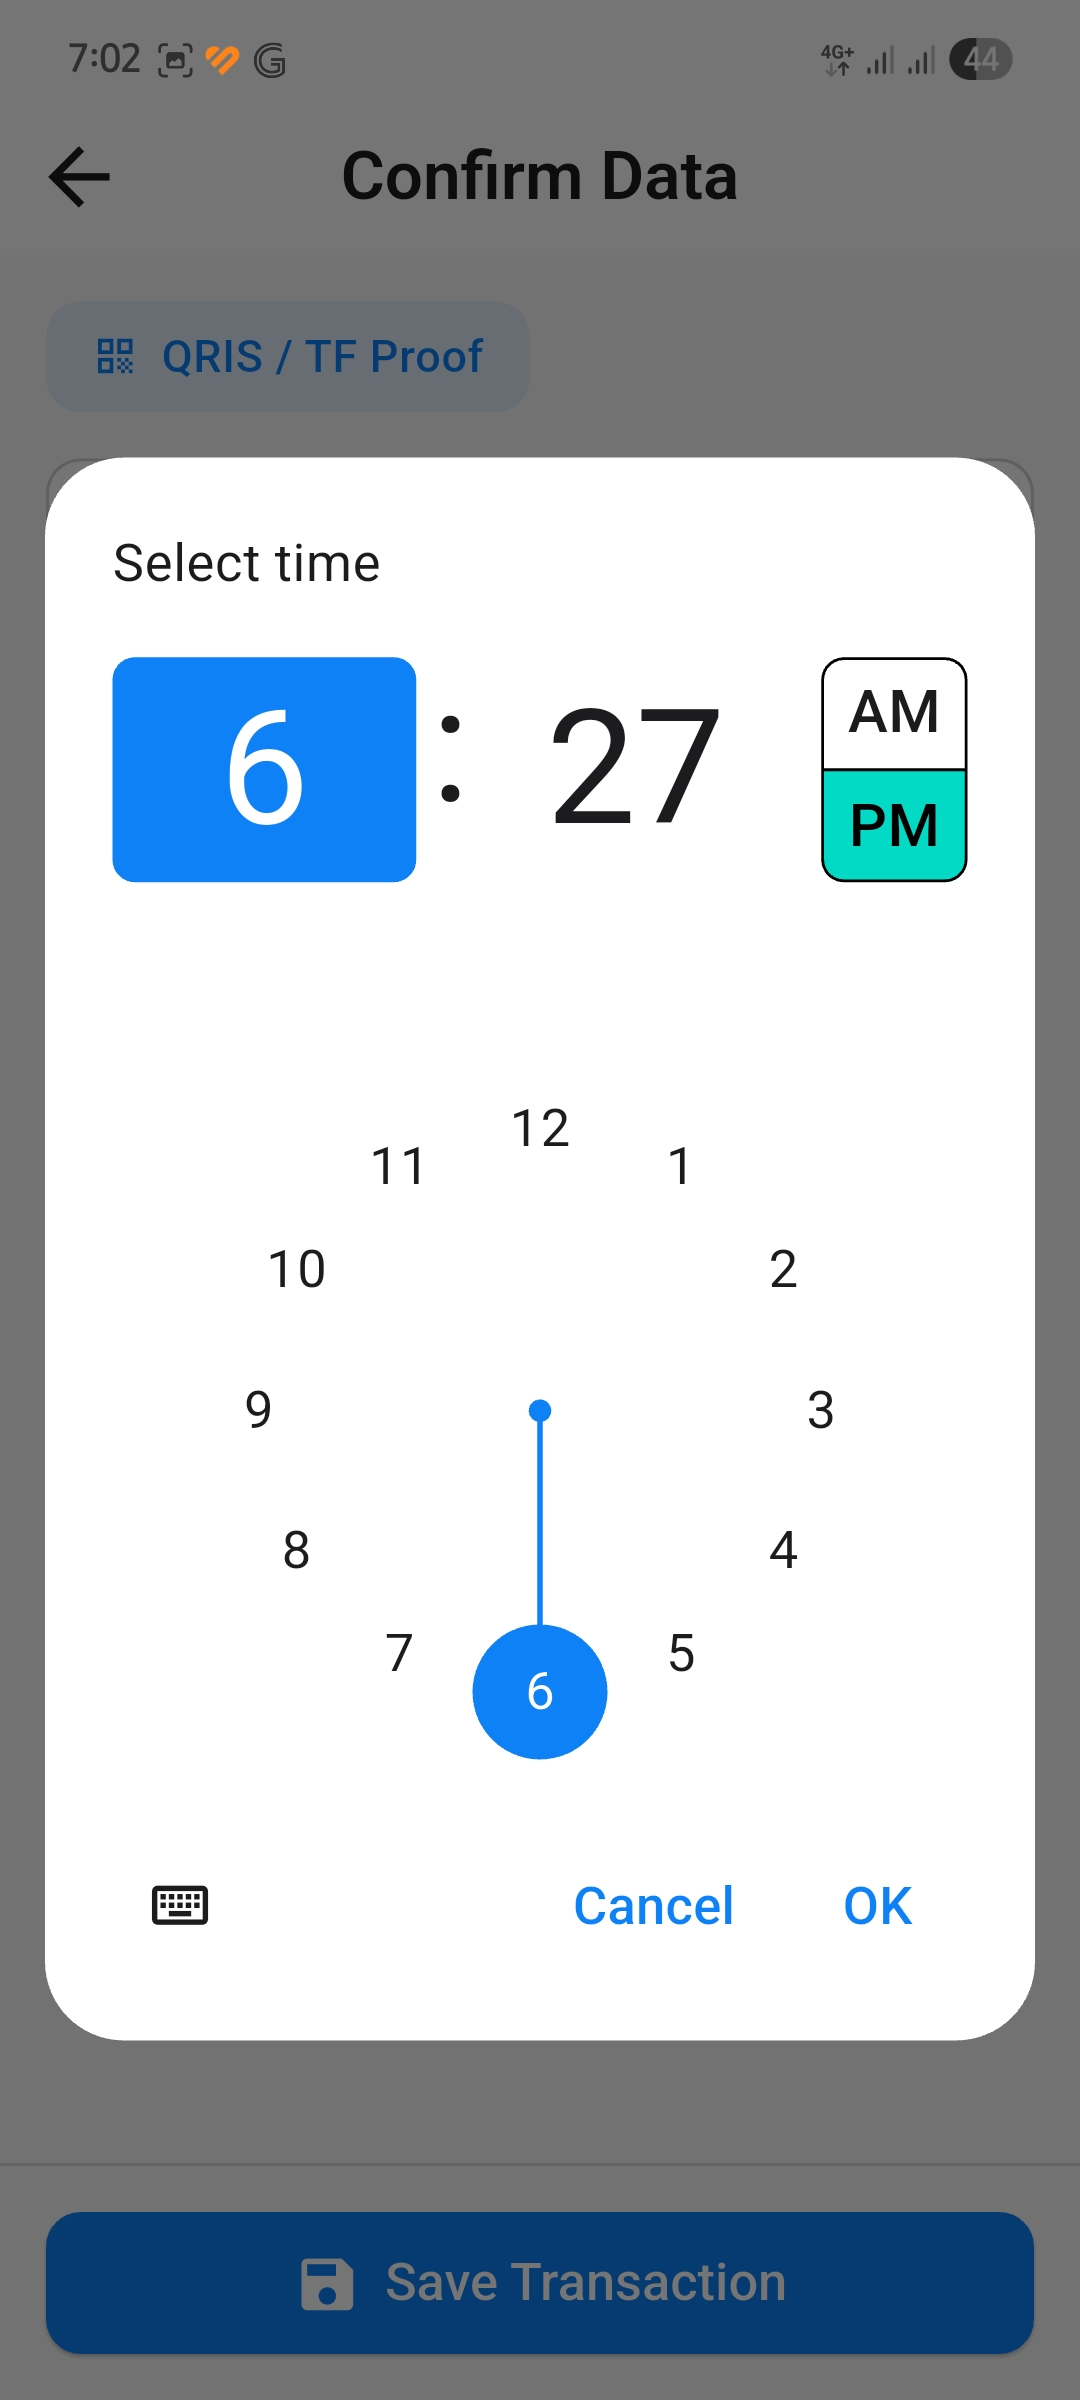
\includegraphics[width=0.33\textwidth]{images/UI/qris-tt.jpg} &
    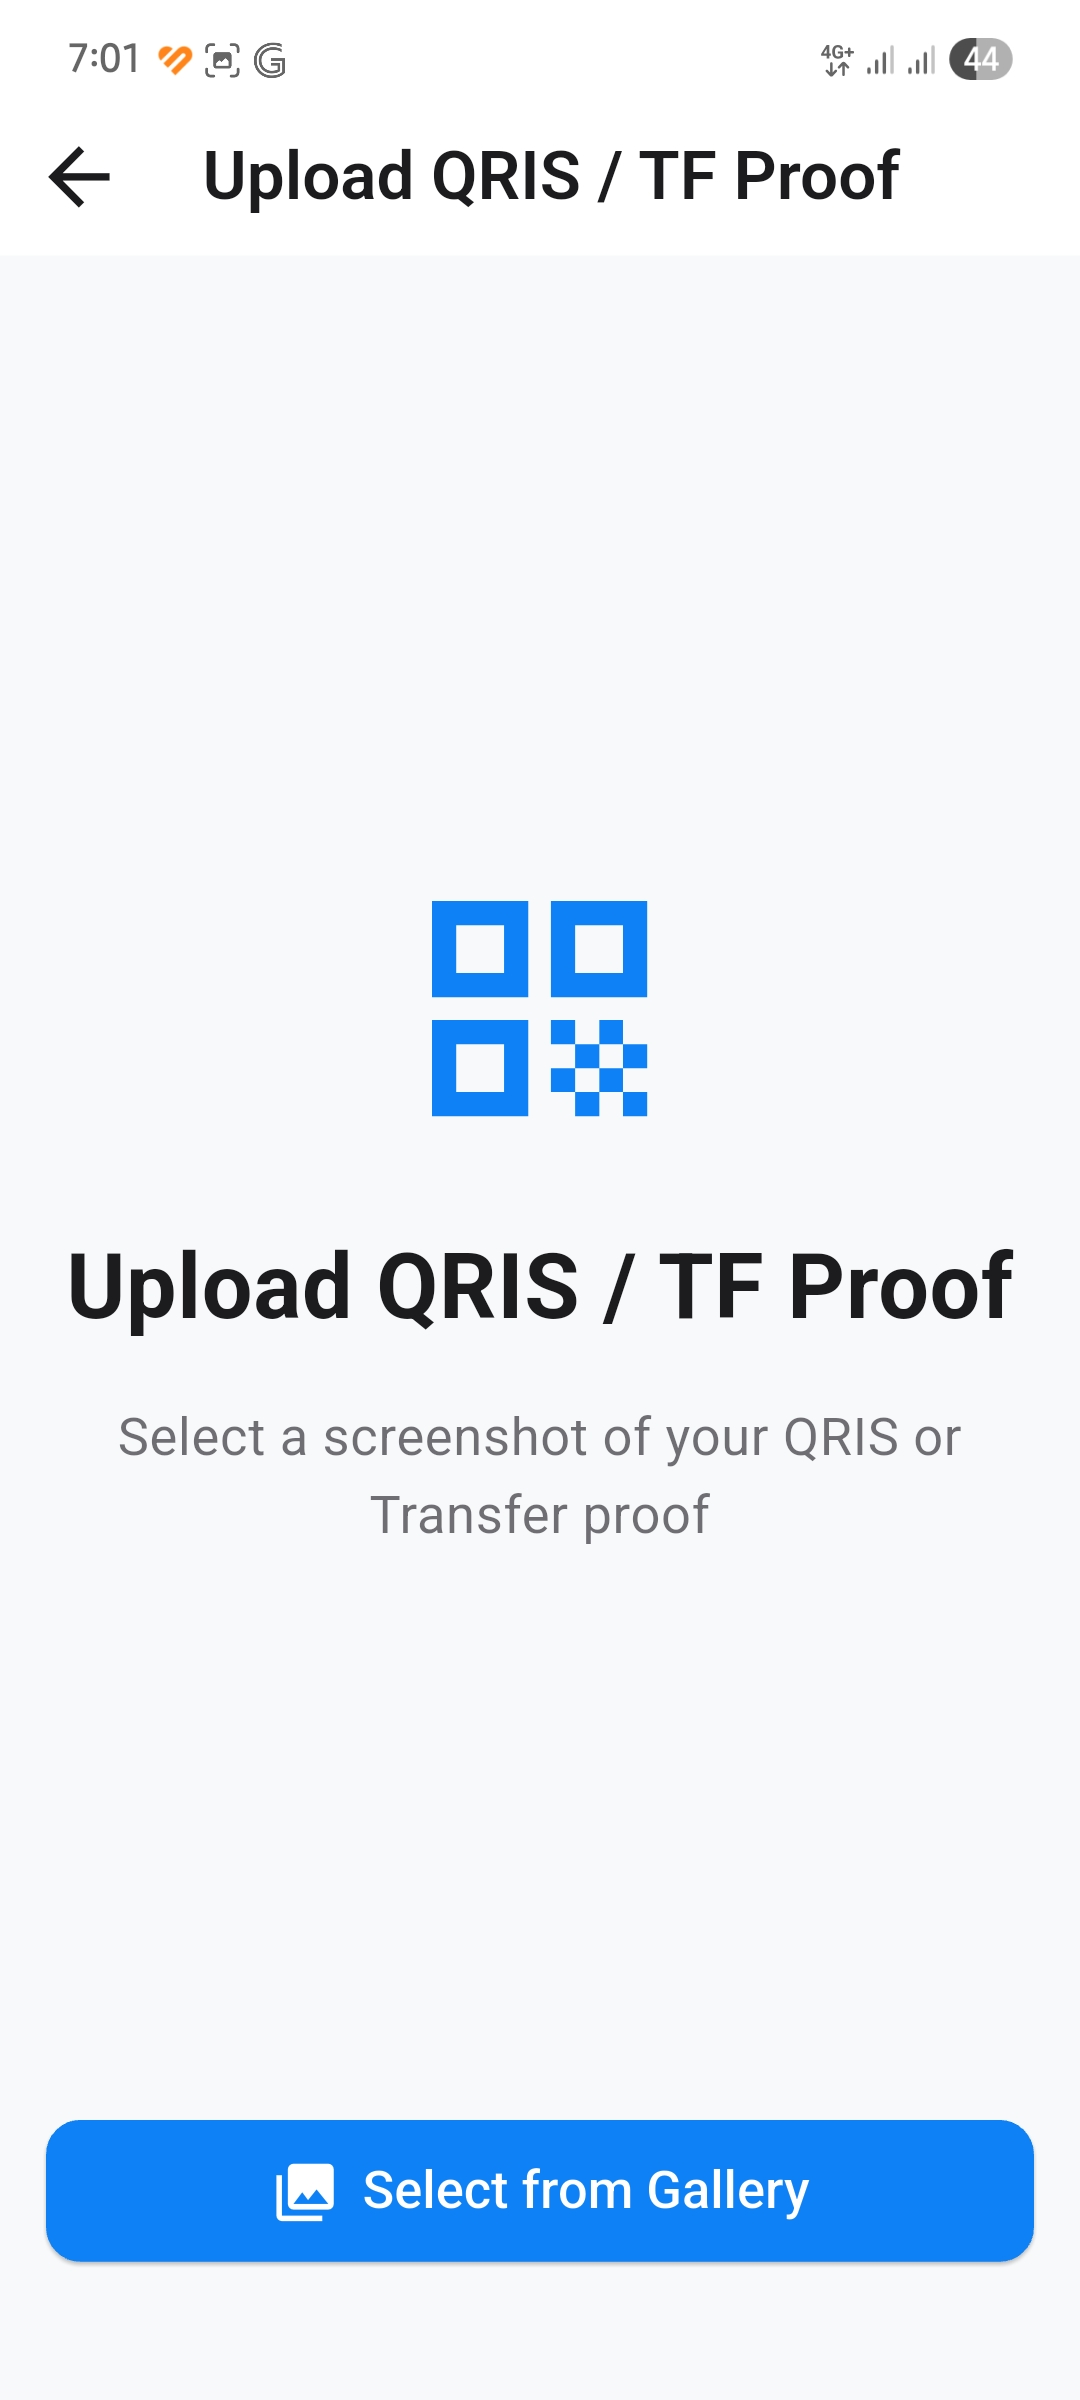
\includegraphics[width=0.33\textwidth]{images/UI/qris-upload.jpg}
    \\
    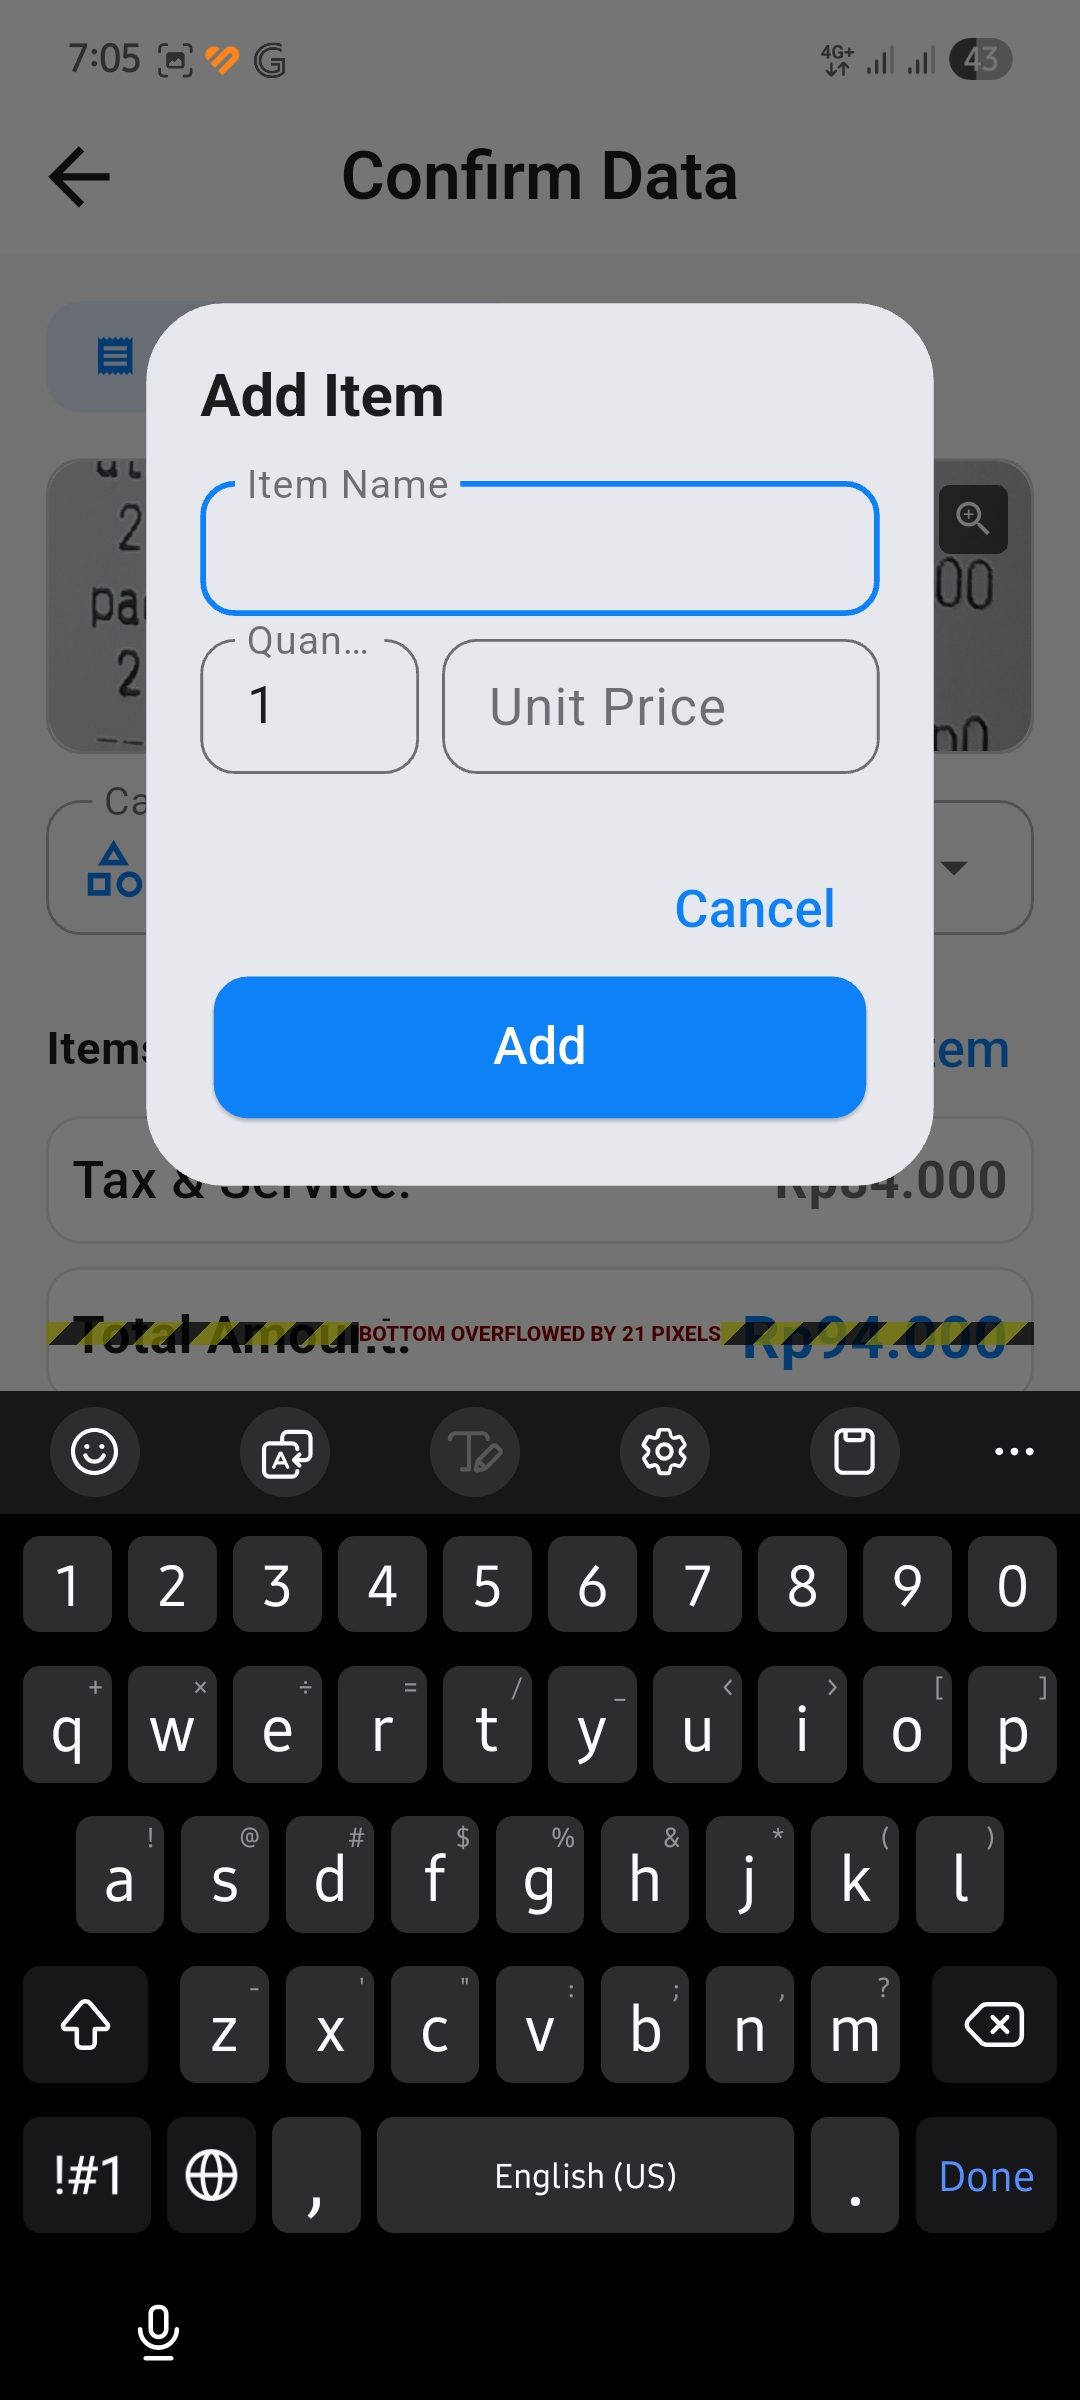
\includegraphics[width=0.33\textwidth]{images/UI/struk-add.jpg} &
    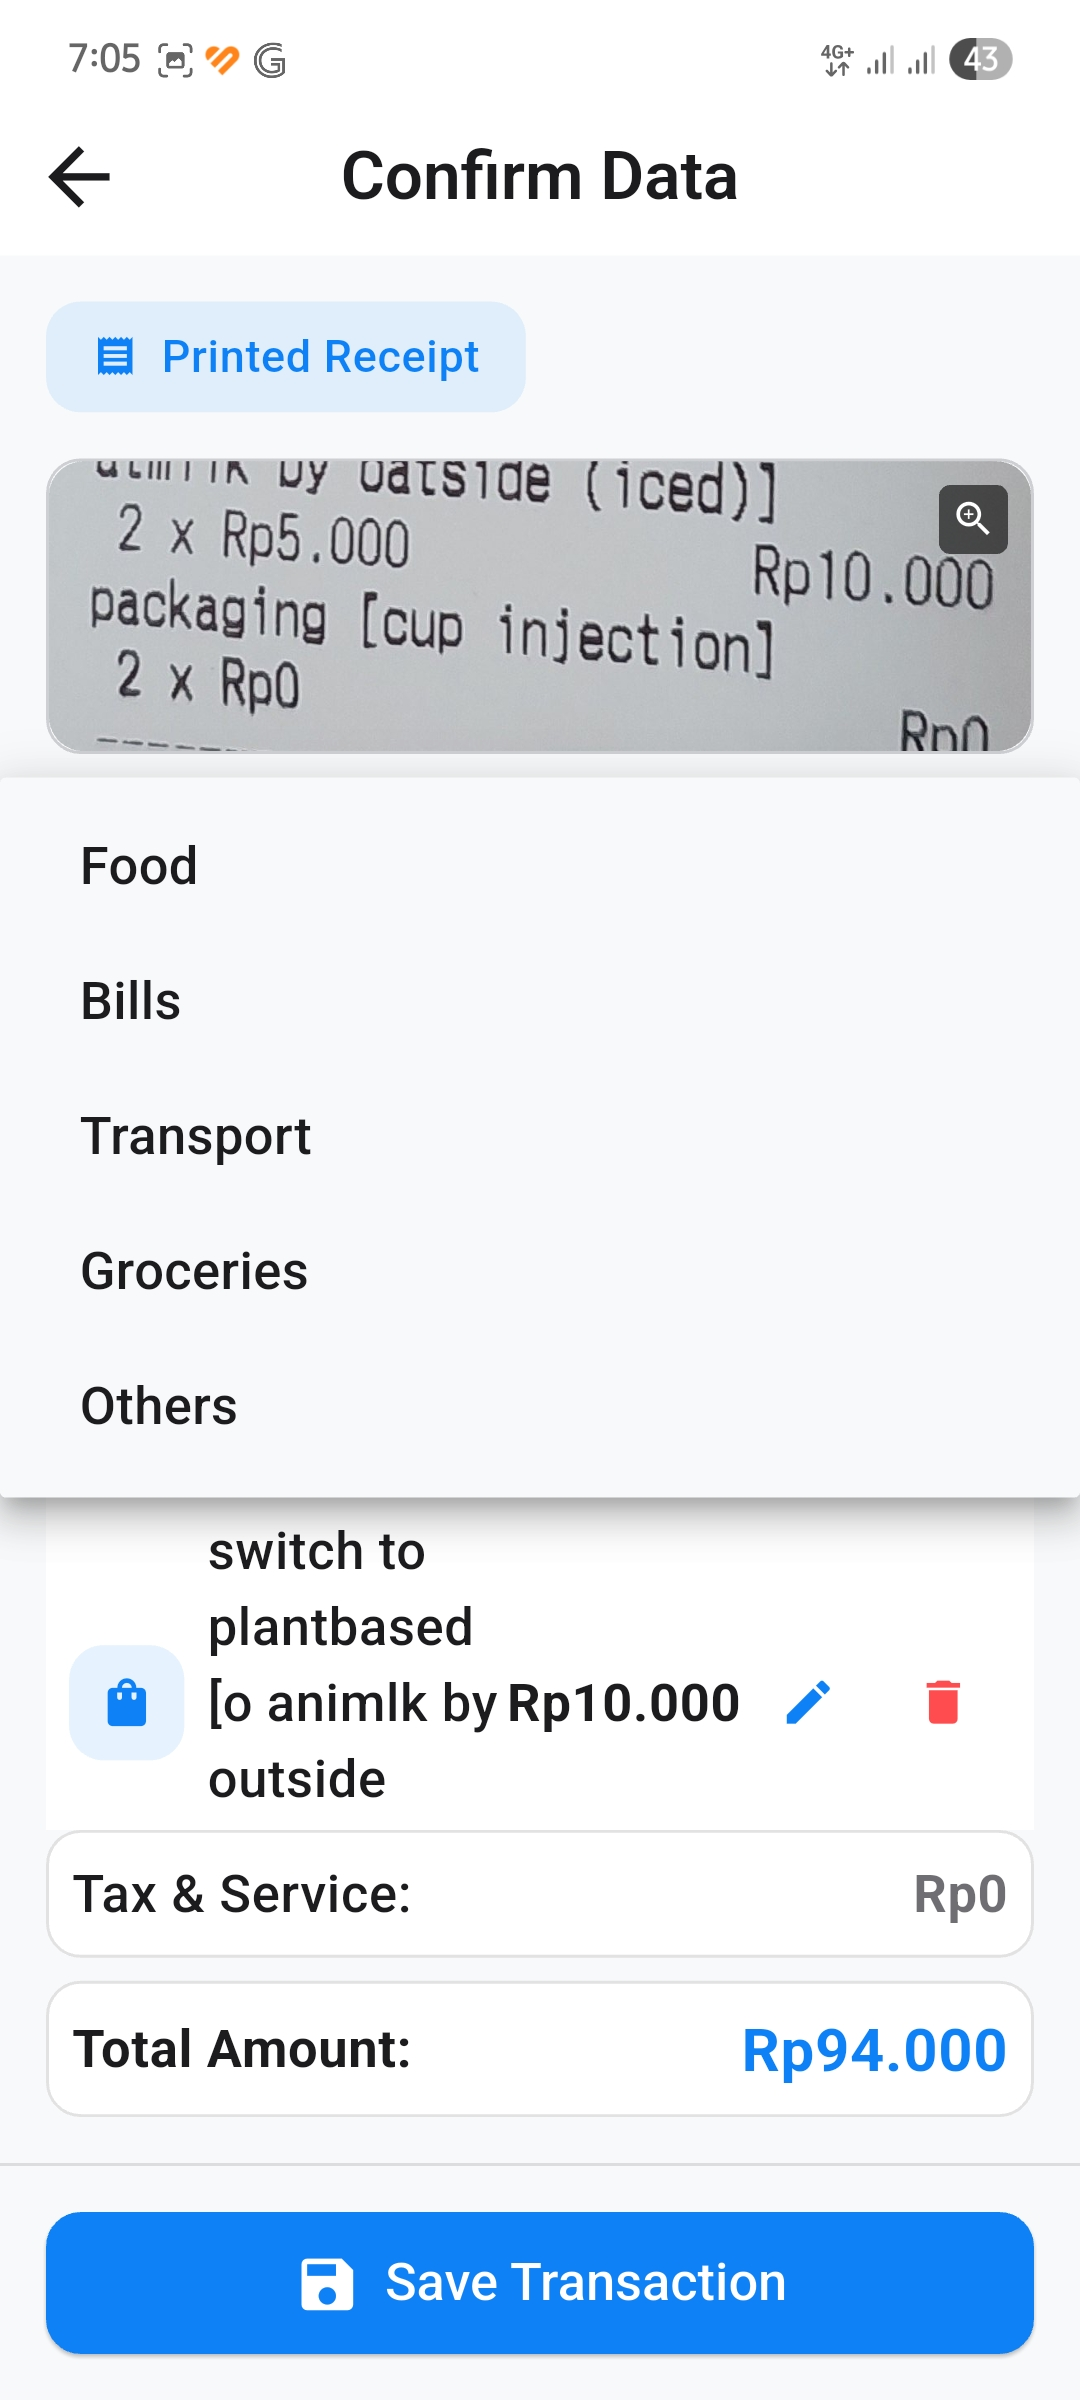
\includegraphics[width=0.33\textwidth]{images/UI/struk-cat.jpg} &
    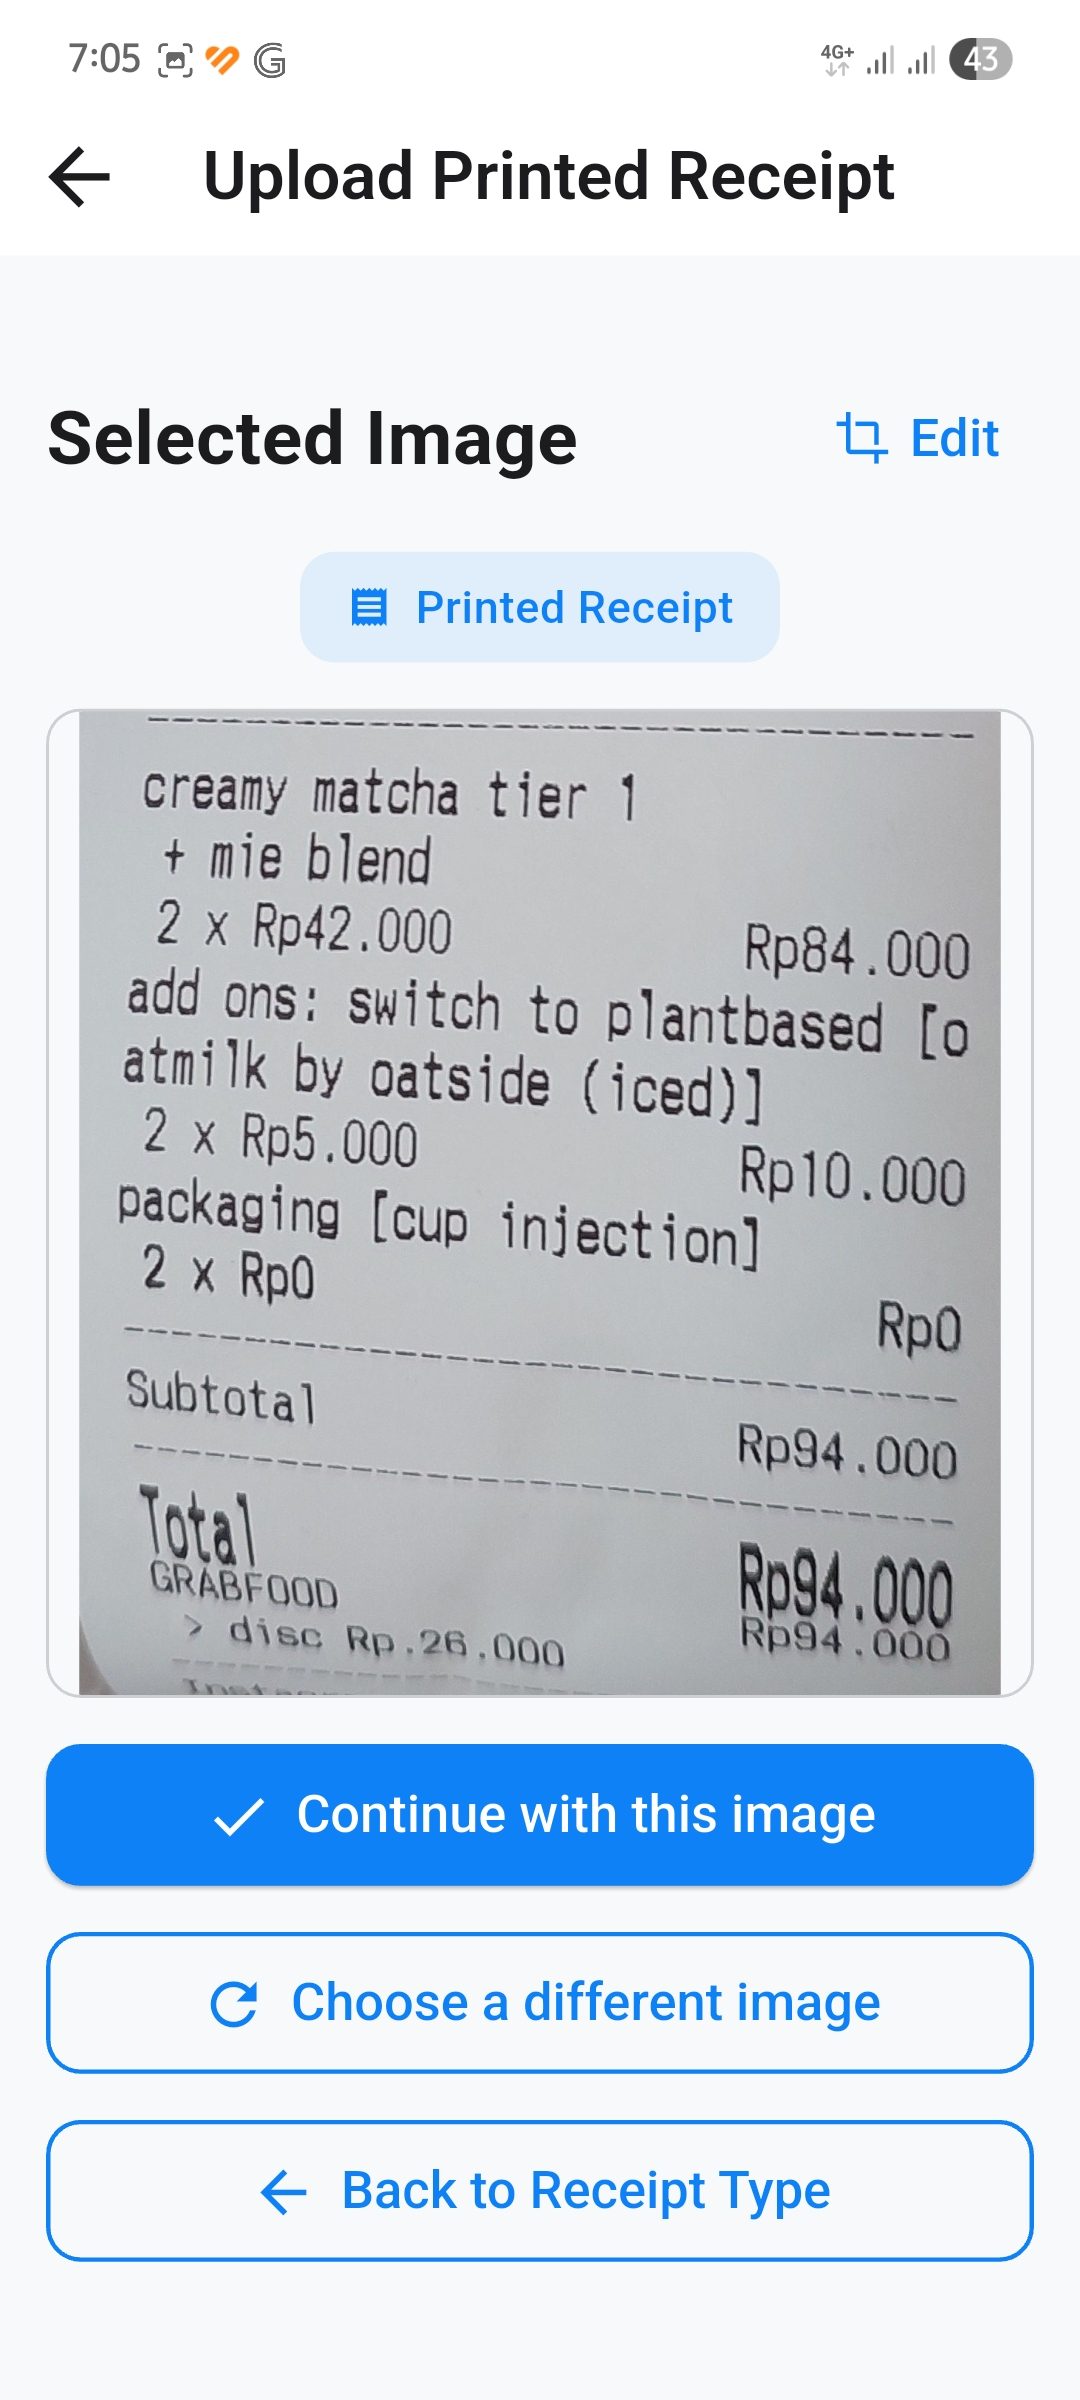
\includegraphics[width=0.33\textwidth]{images/UI/struk-confirm.jpg} \\
\end{tabular}

\begin{tabular}{lll}
    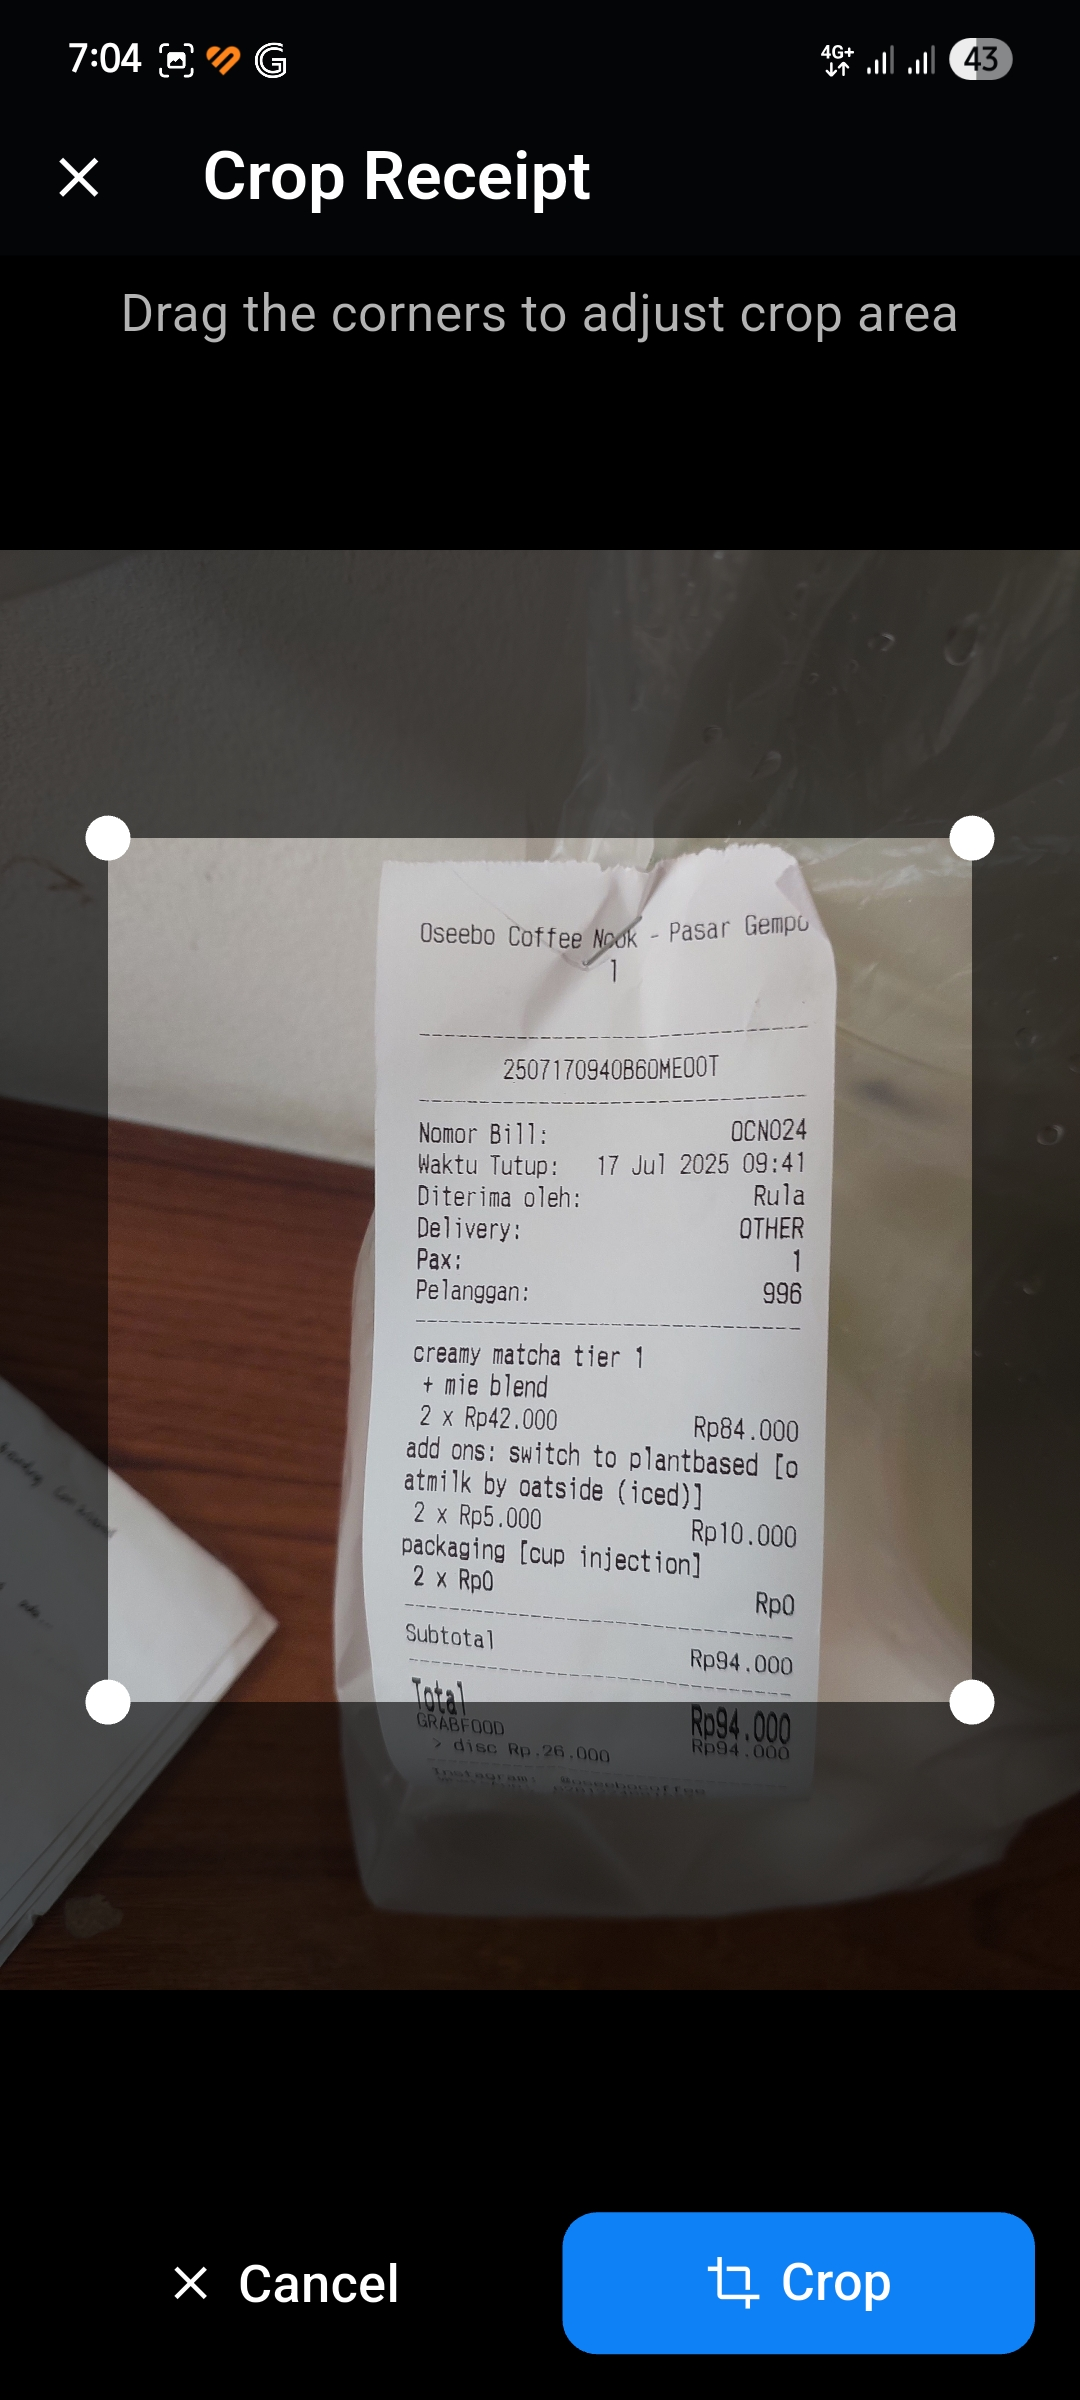
\includegraphics[width=0.33\textwidth]{images/UI/struk-crop.jpg} &
    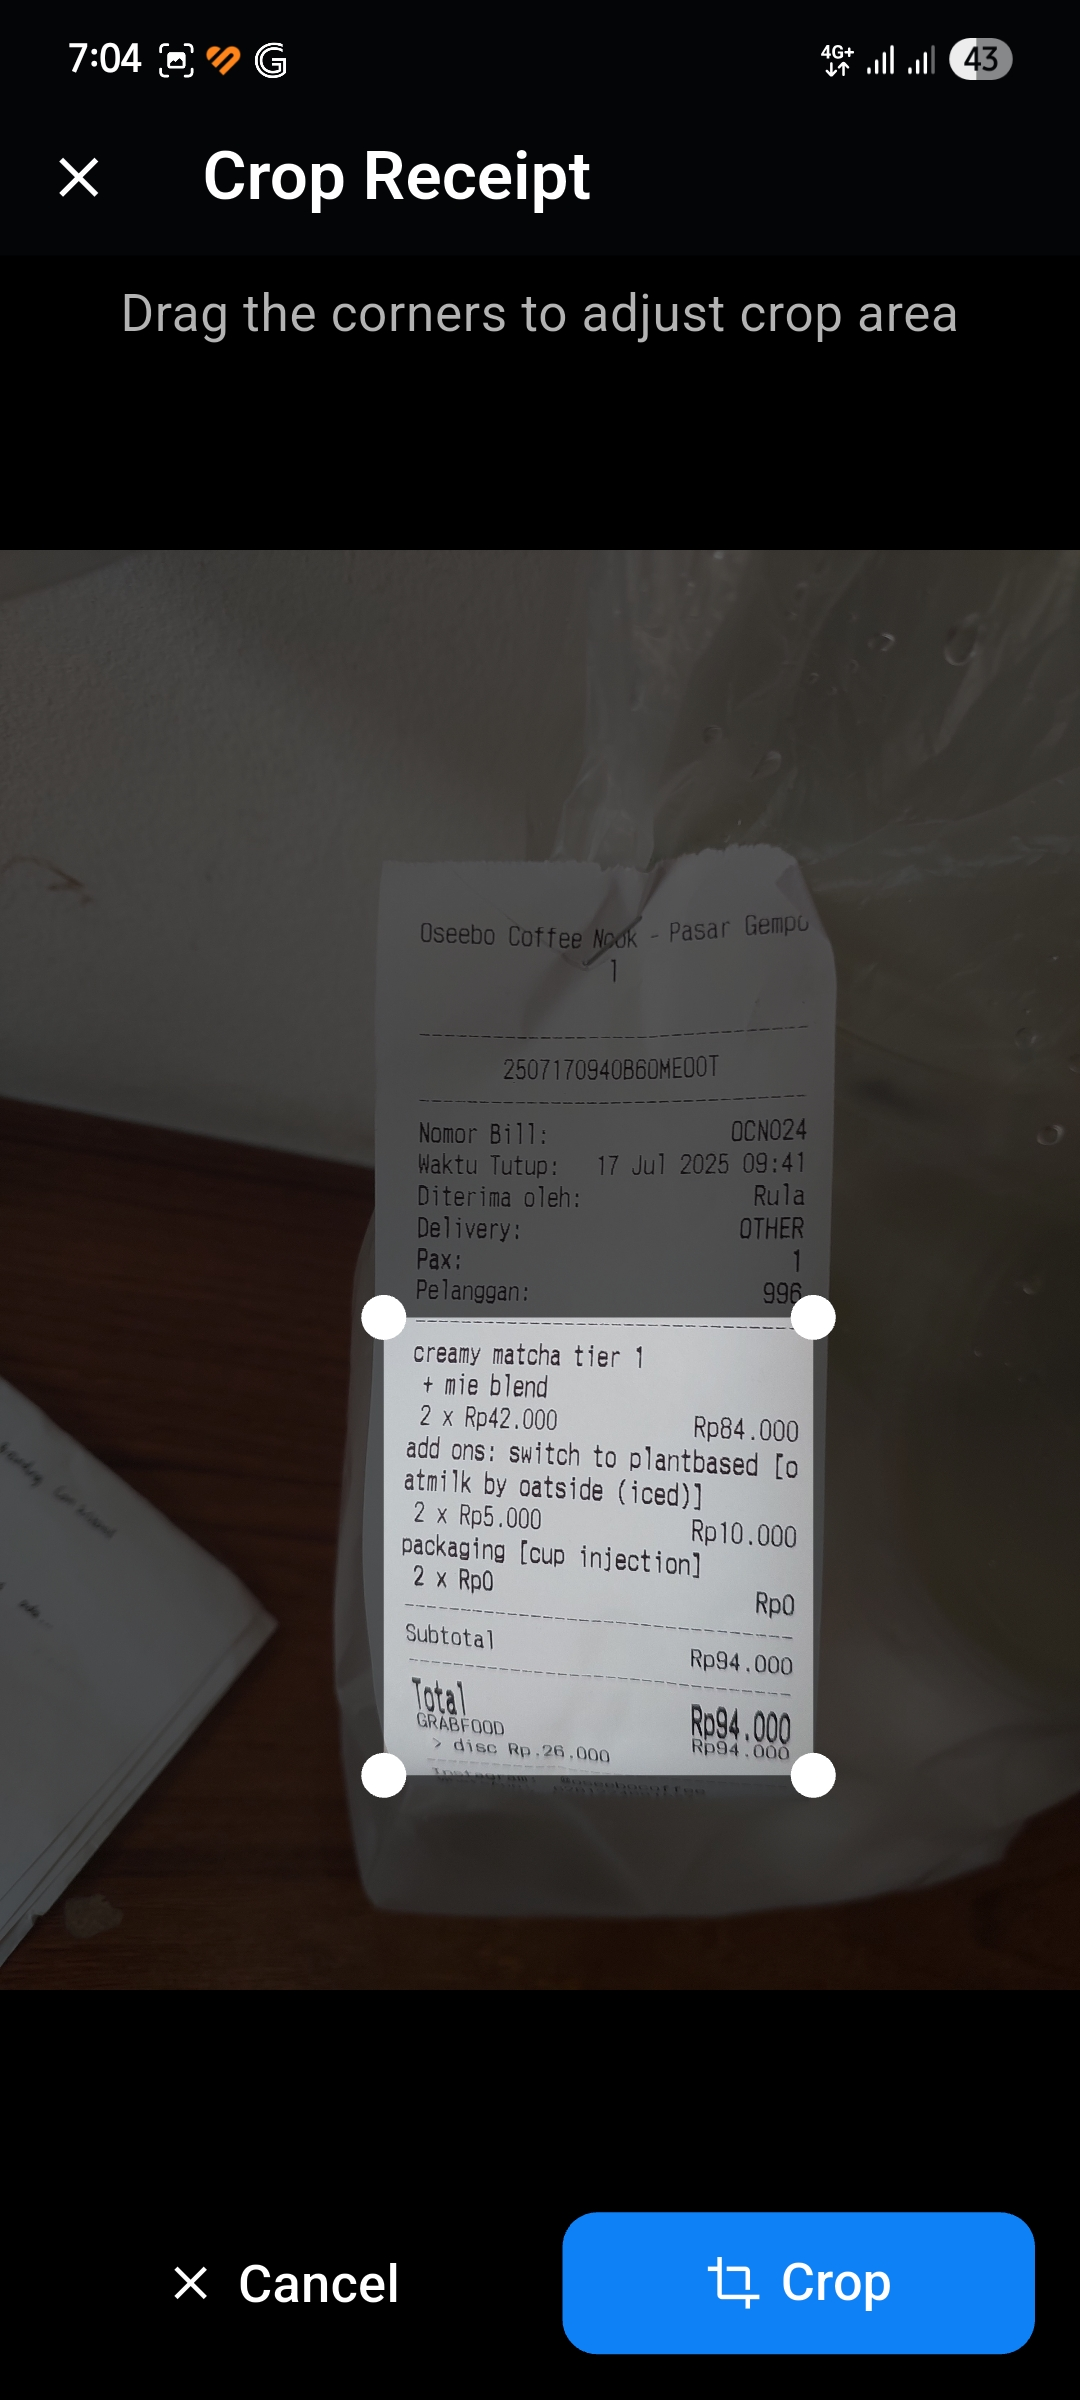
\includegraphics[width=0.33\textwidth]{images/UI/struk-cropped.jpg} &
    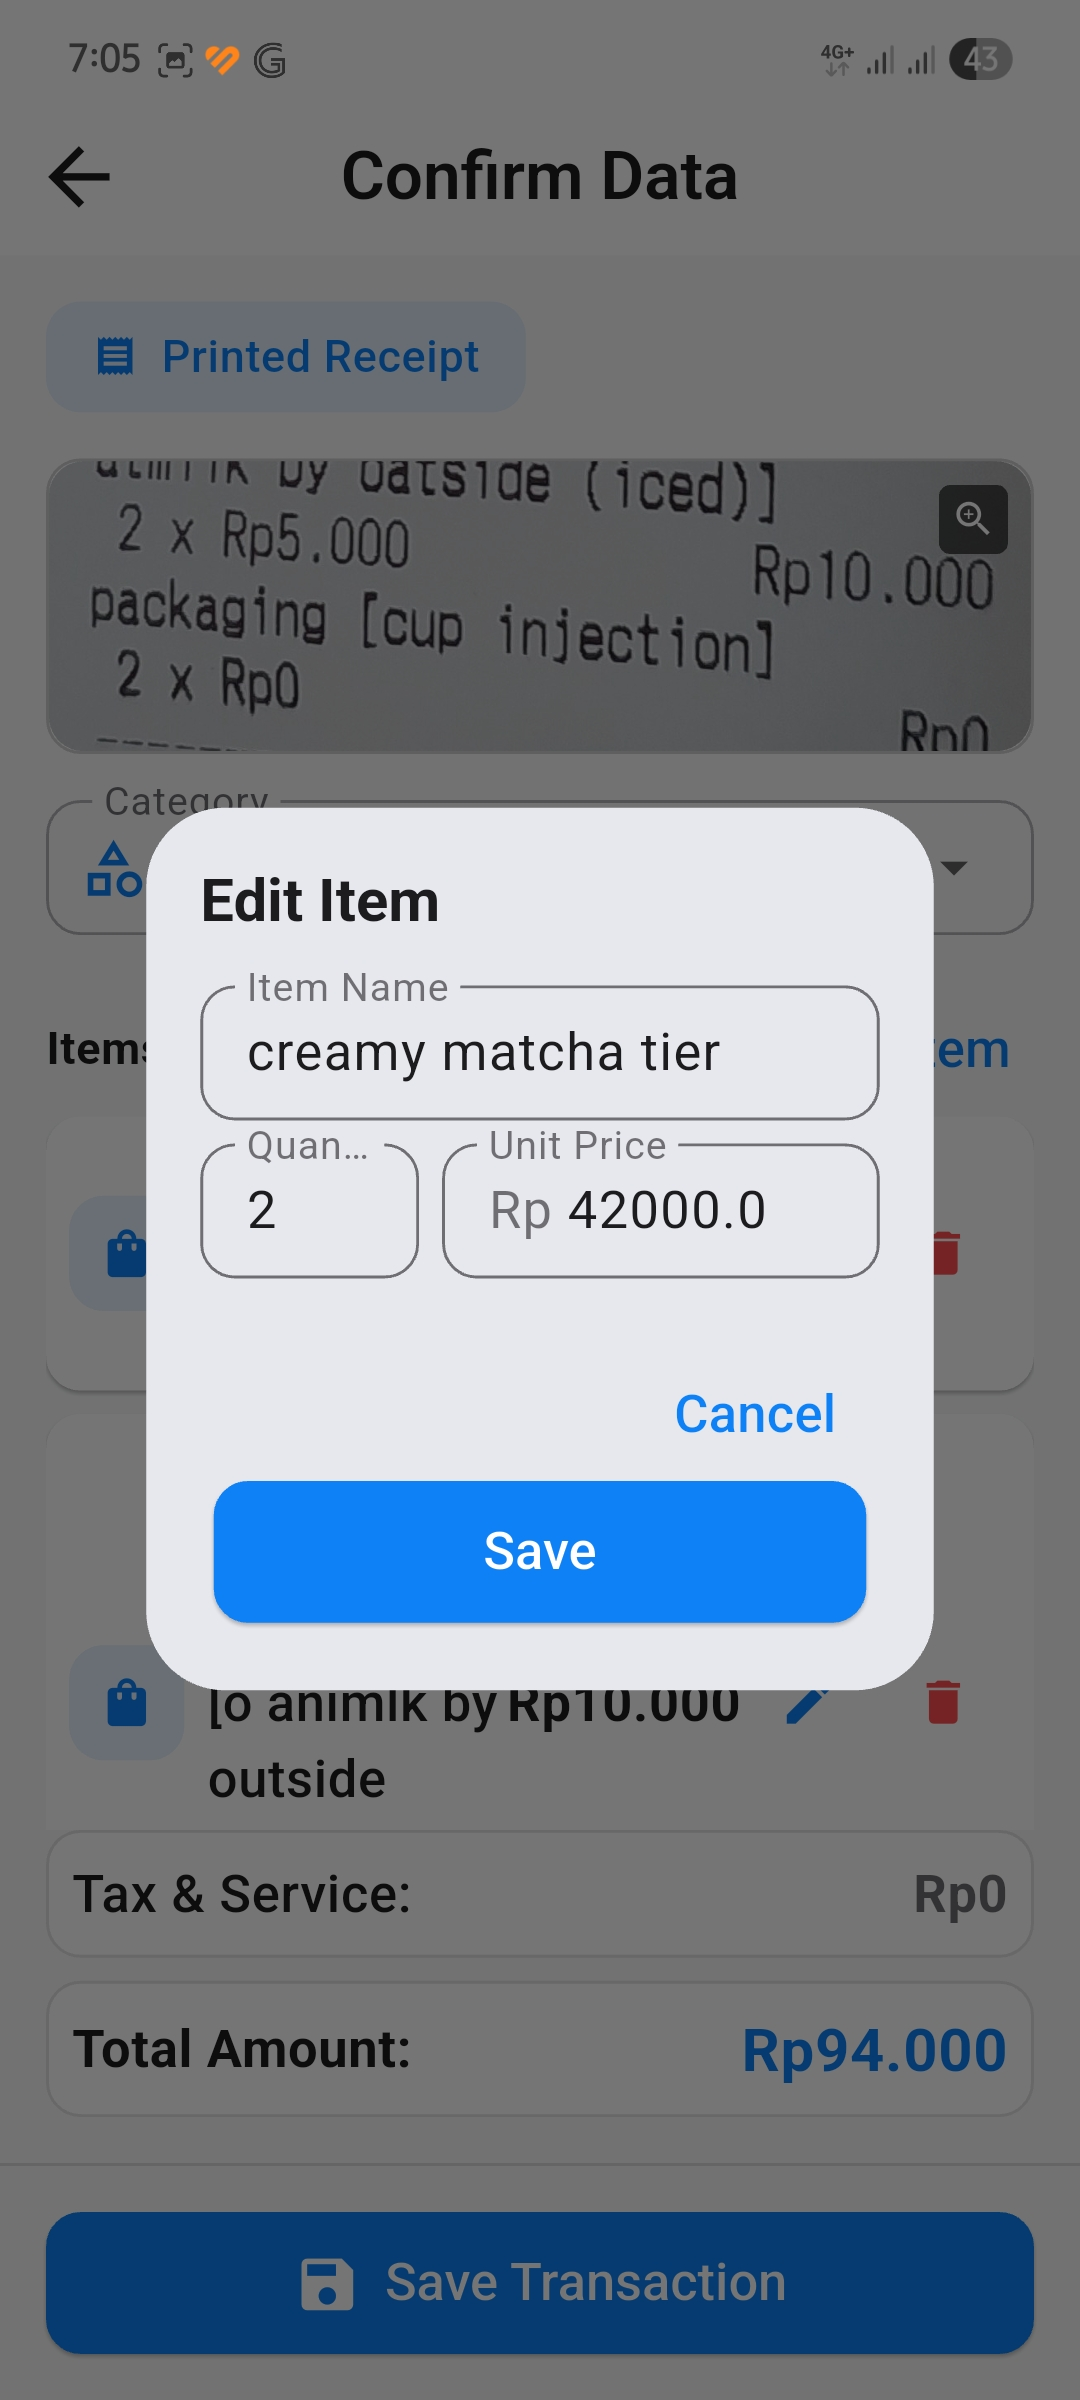
\includegraphics[width=0.33\textwidth]{images/UI/struk-edit.jpg}
    \\
    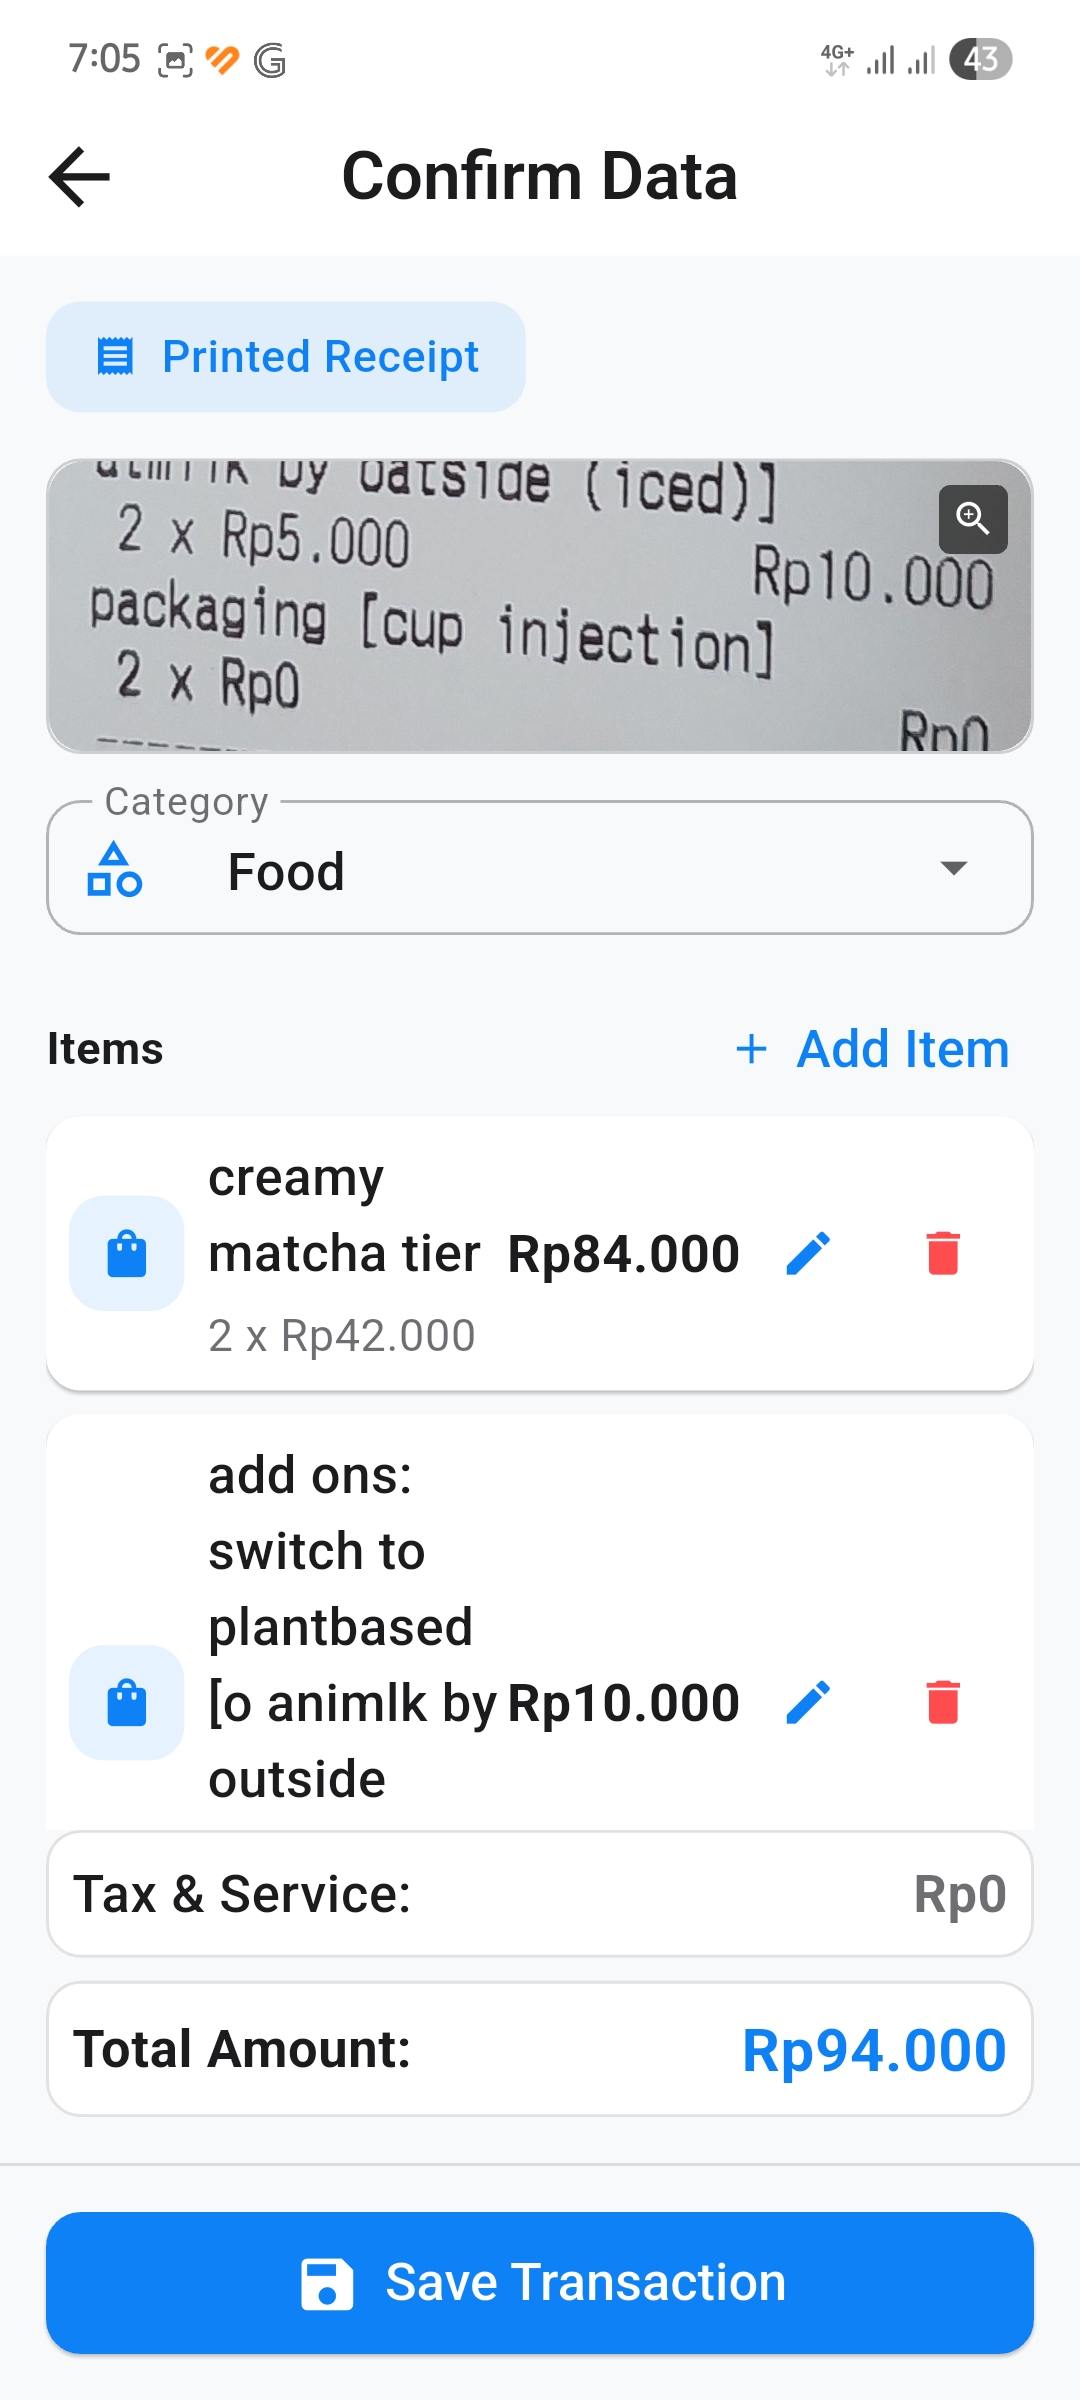
\includegraphics[width=0.33\textwidth]{images/UI/struk-mapping.jpg} &
    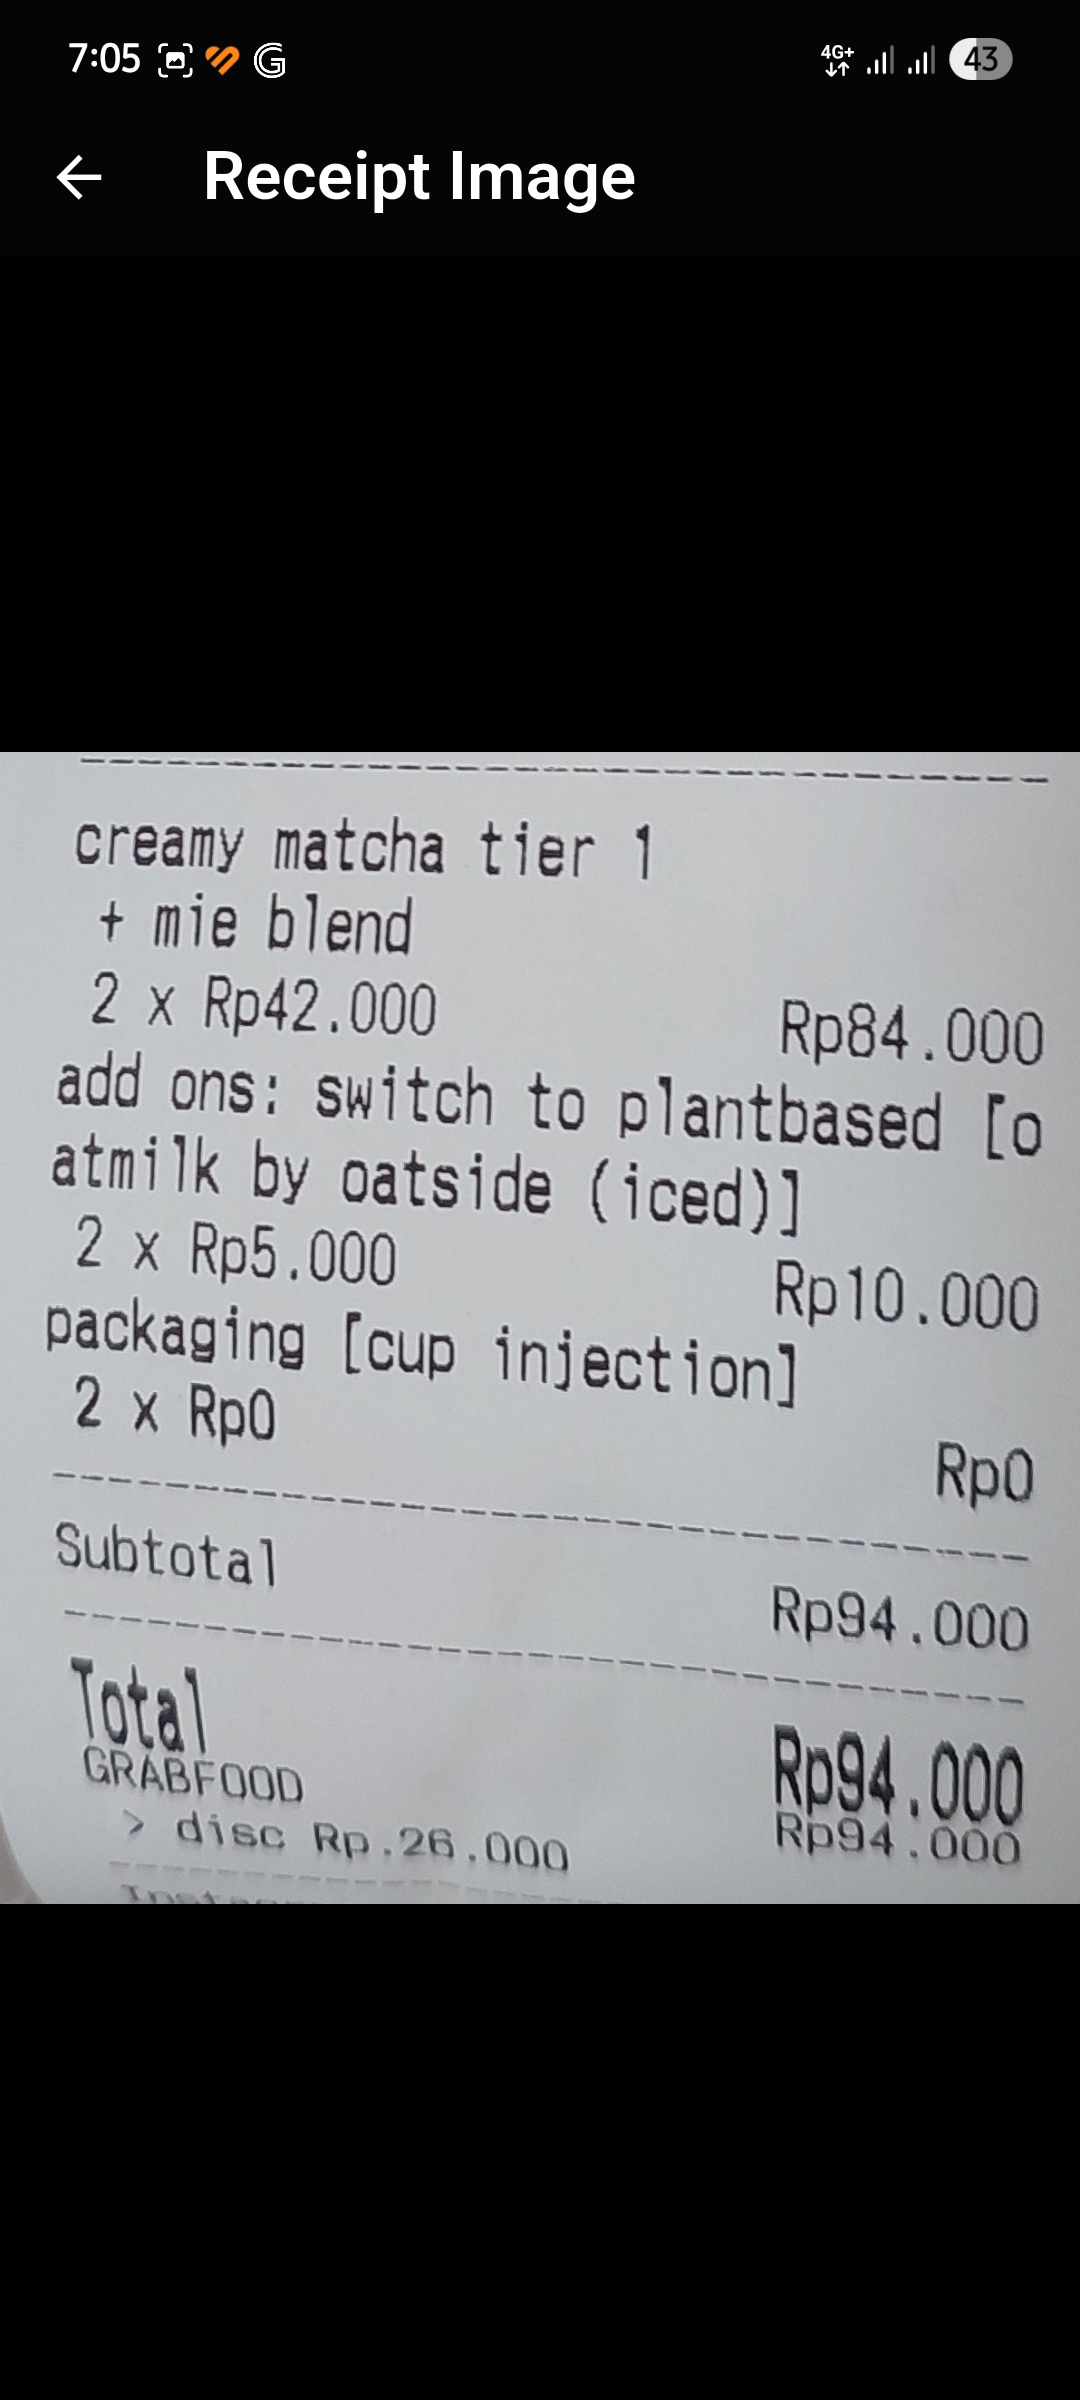
\includegraphics[width=0.33\textwidth]{images/UI/struk-review.jpg} &
    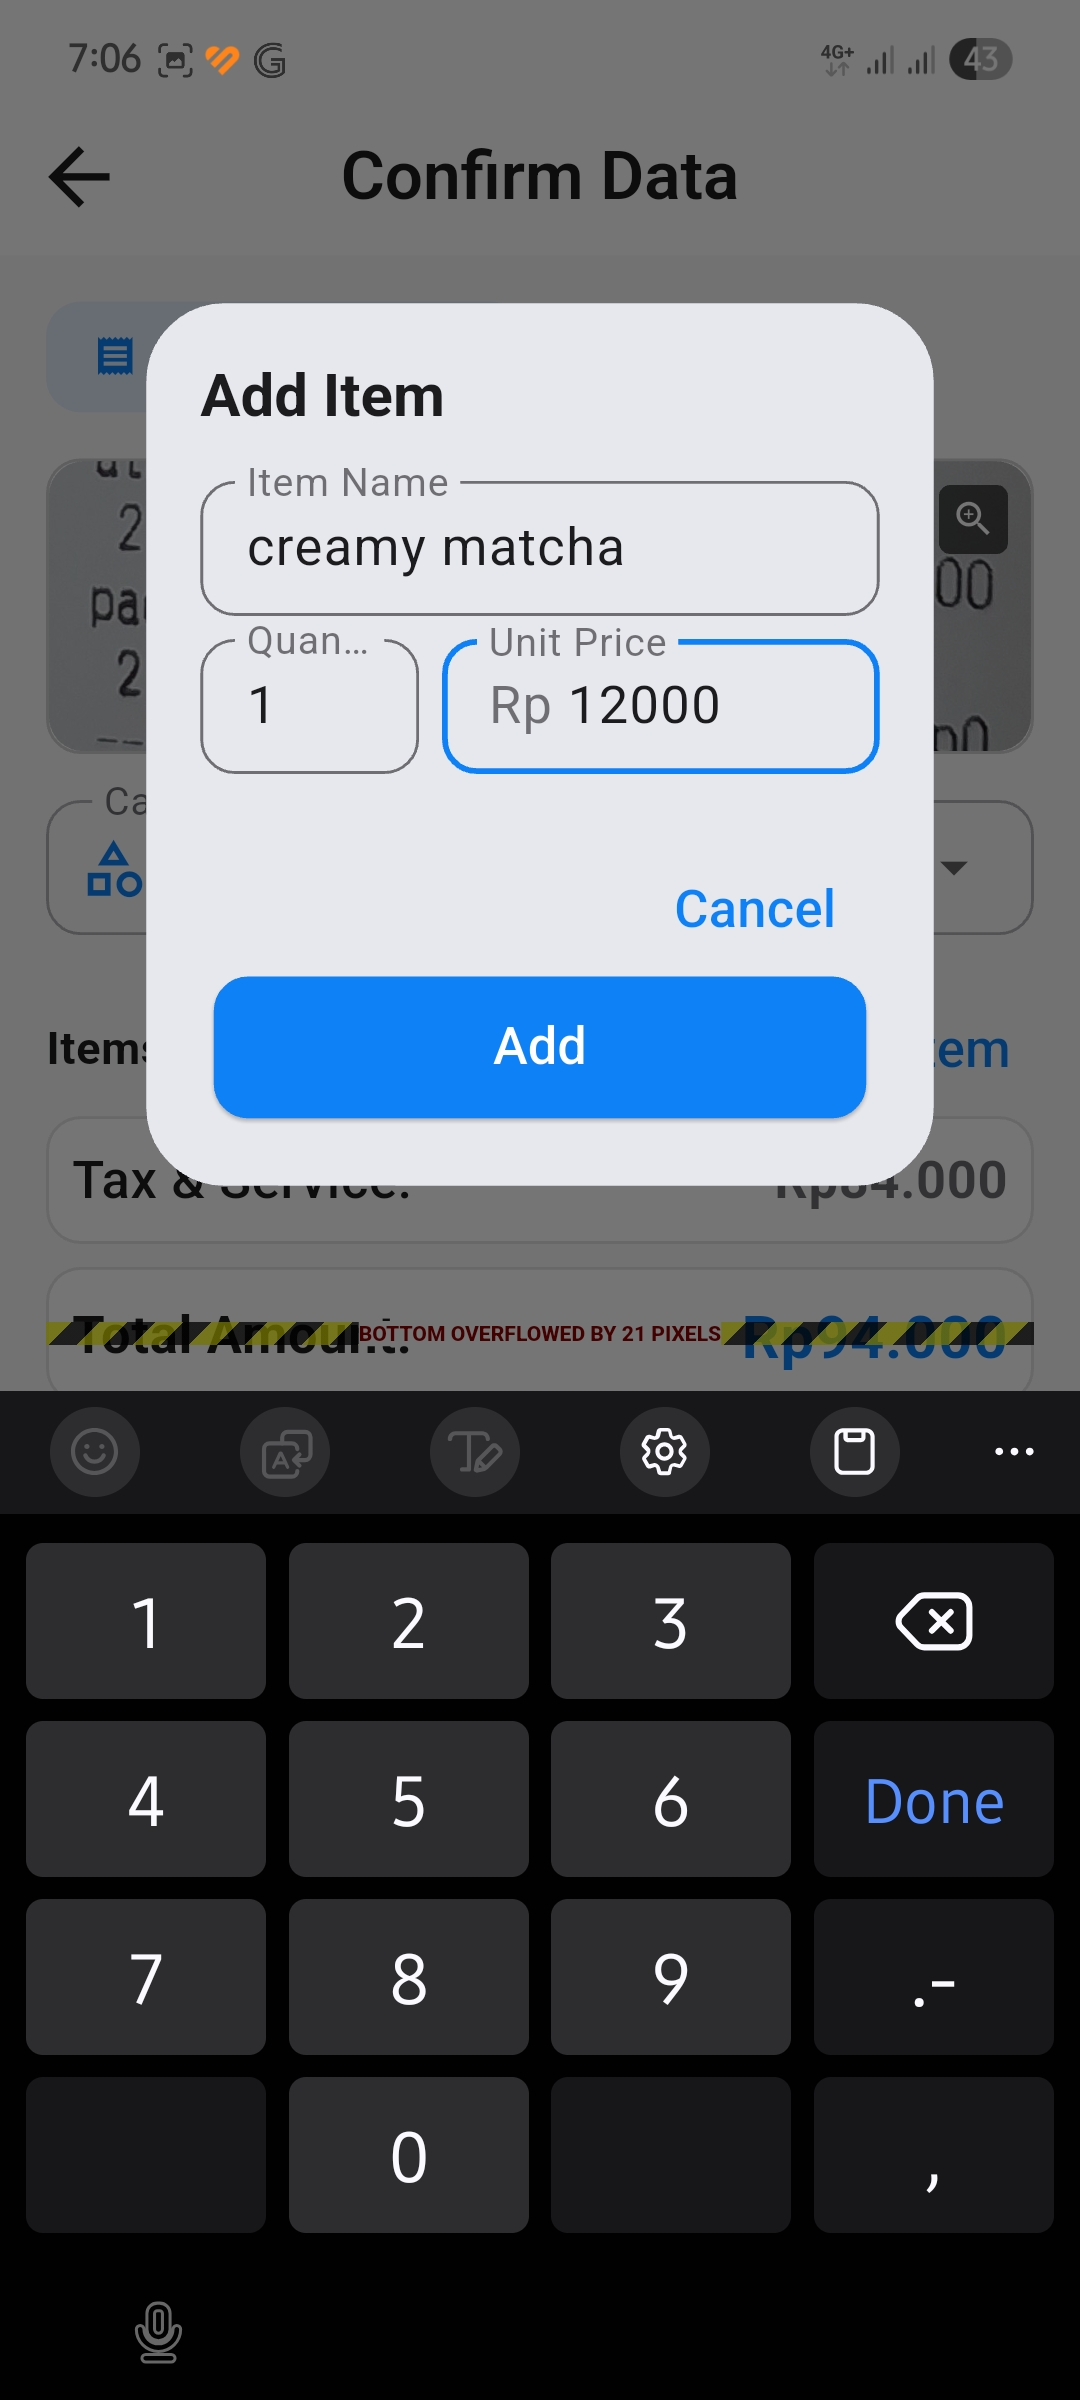
\includegraphics[width=0.33\textwidth]{images/UI/struk-unit.jpg} \\
\end{tabular}
\begin{tabular}{lll}
    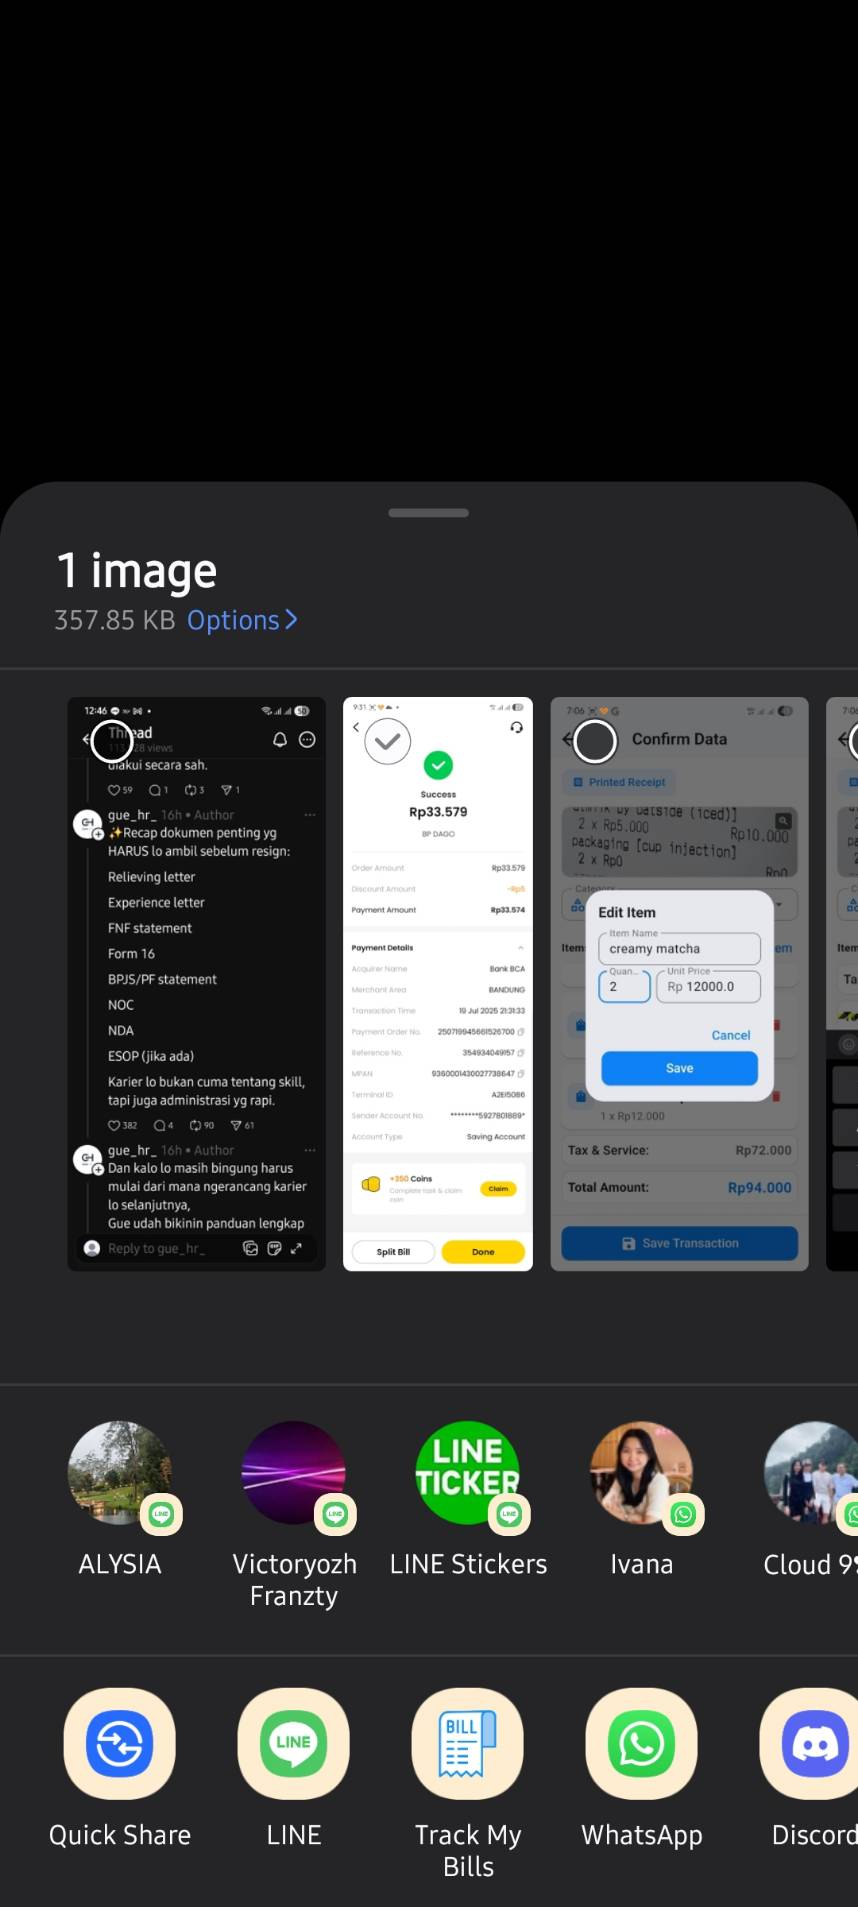
\includegraphics[width=0.33\textwidth]{images/UI/sharing-intent.jpg} &
    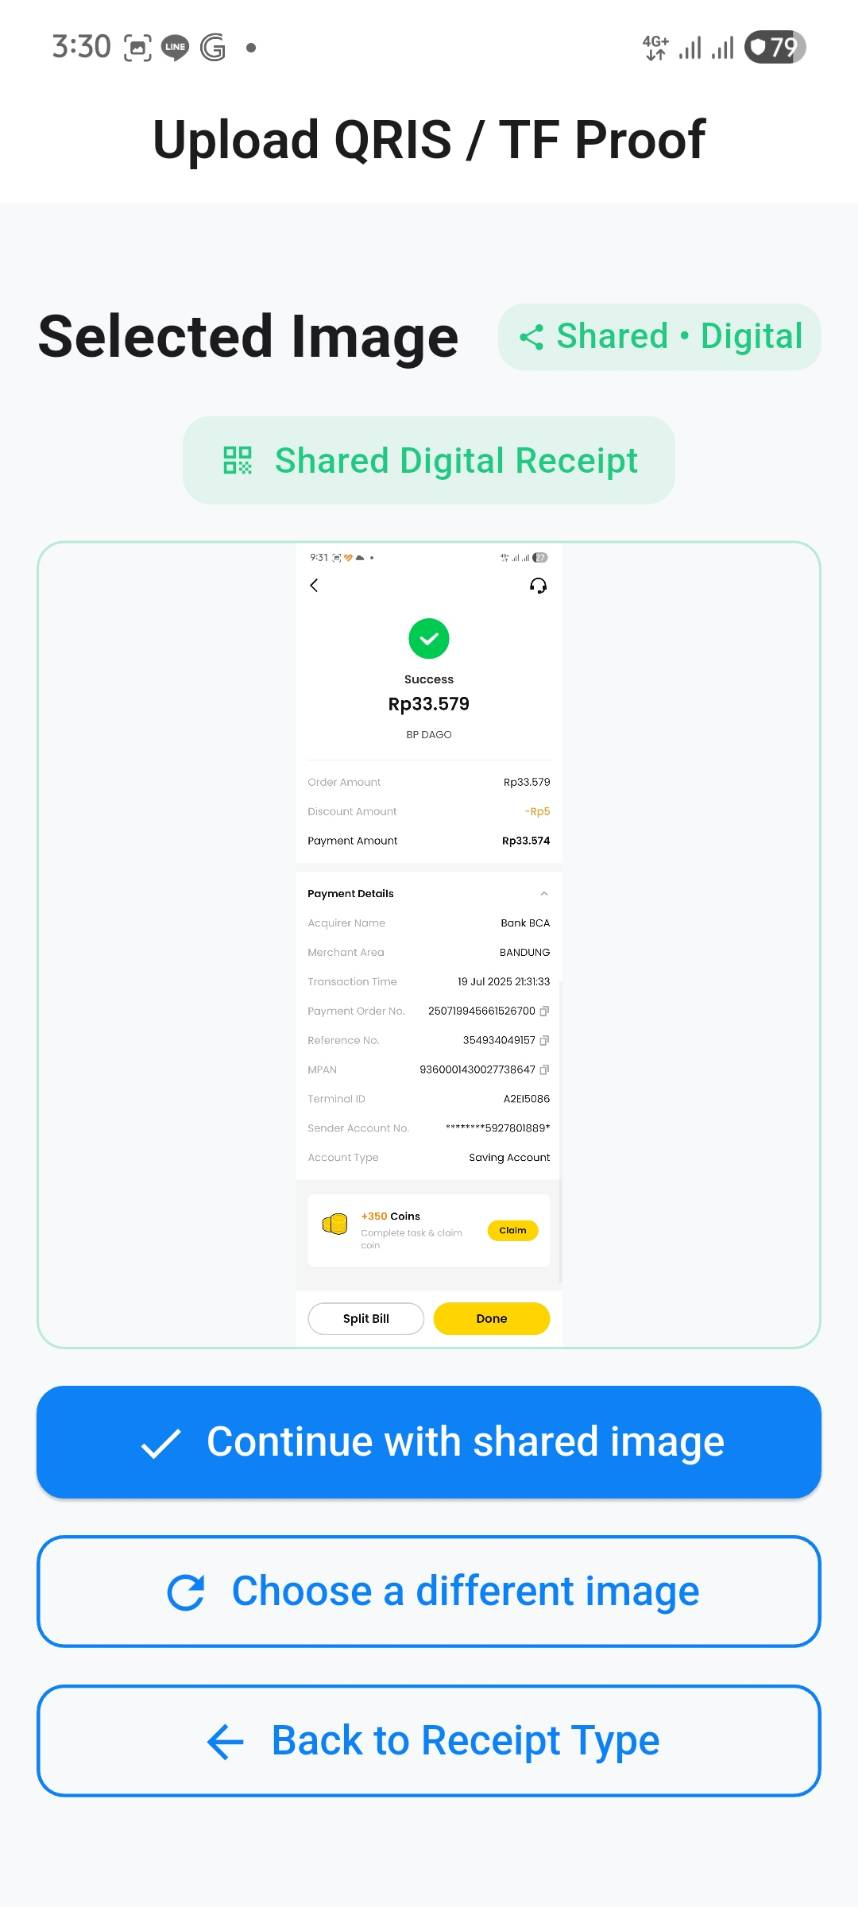
\includegraphics[width=0.33\textwidth]{images/UI/shared-confirm.jpg} &
    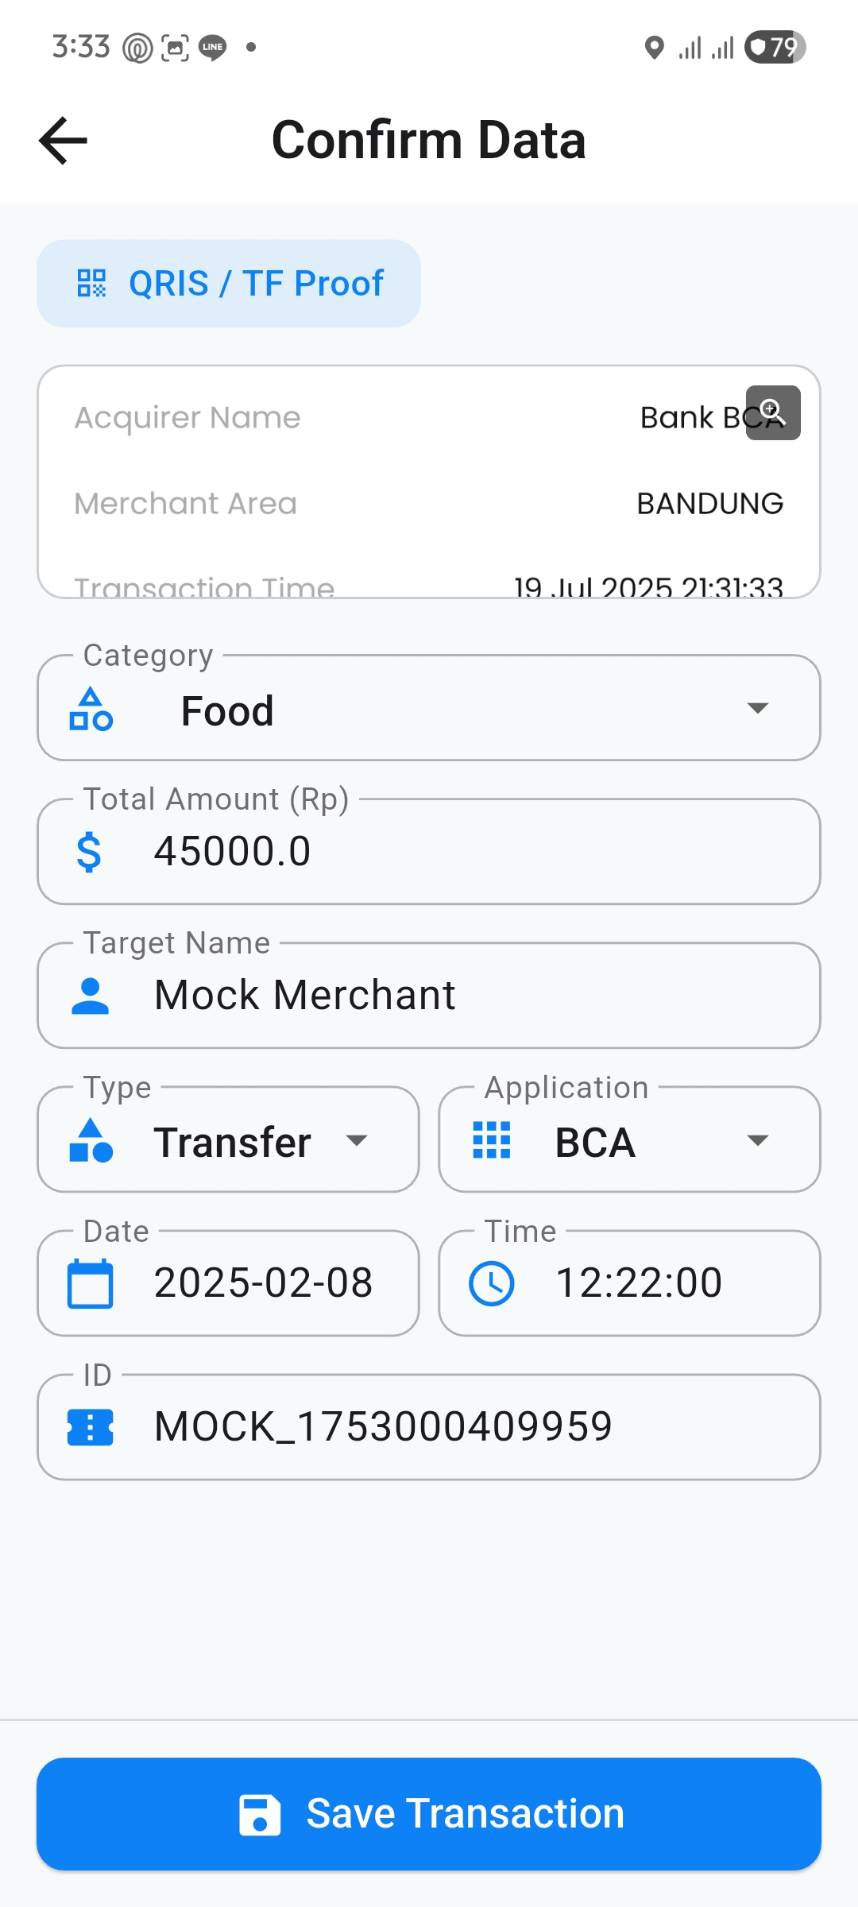
\includegraphics[width=0.33\textwidth]{images/UI/mock-data.jpg}
    \\
\end{tabular}
\chapter{Hasil Kuesioner Evaluasi Pengguna}

\begin{tabular}{c}
	\begin{minipage}{\linewidth}
		\centering
    	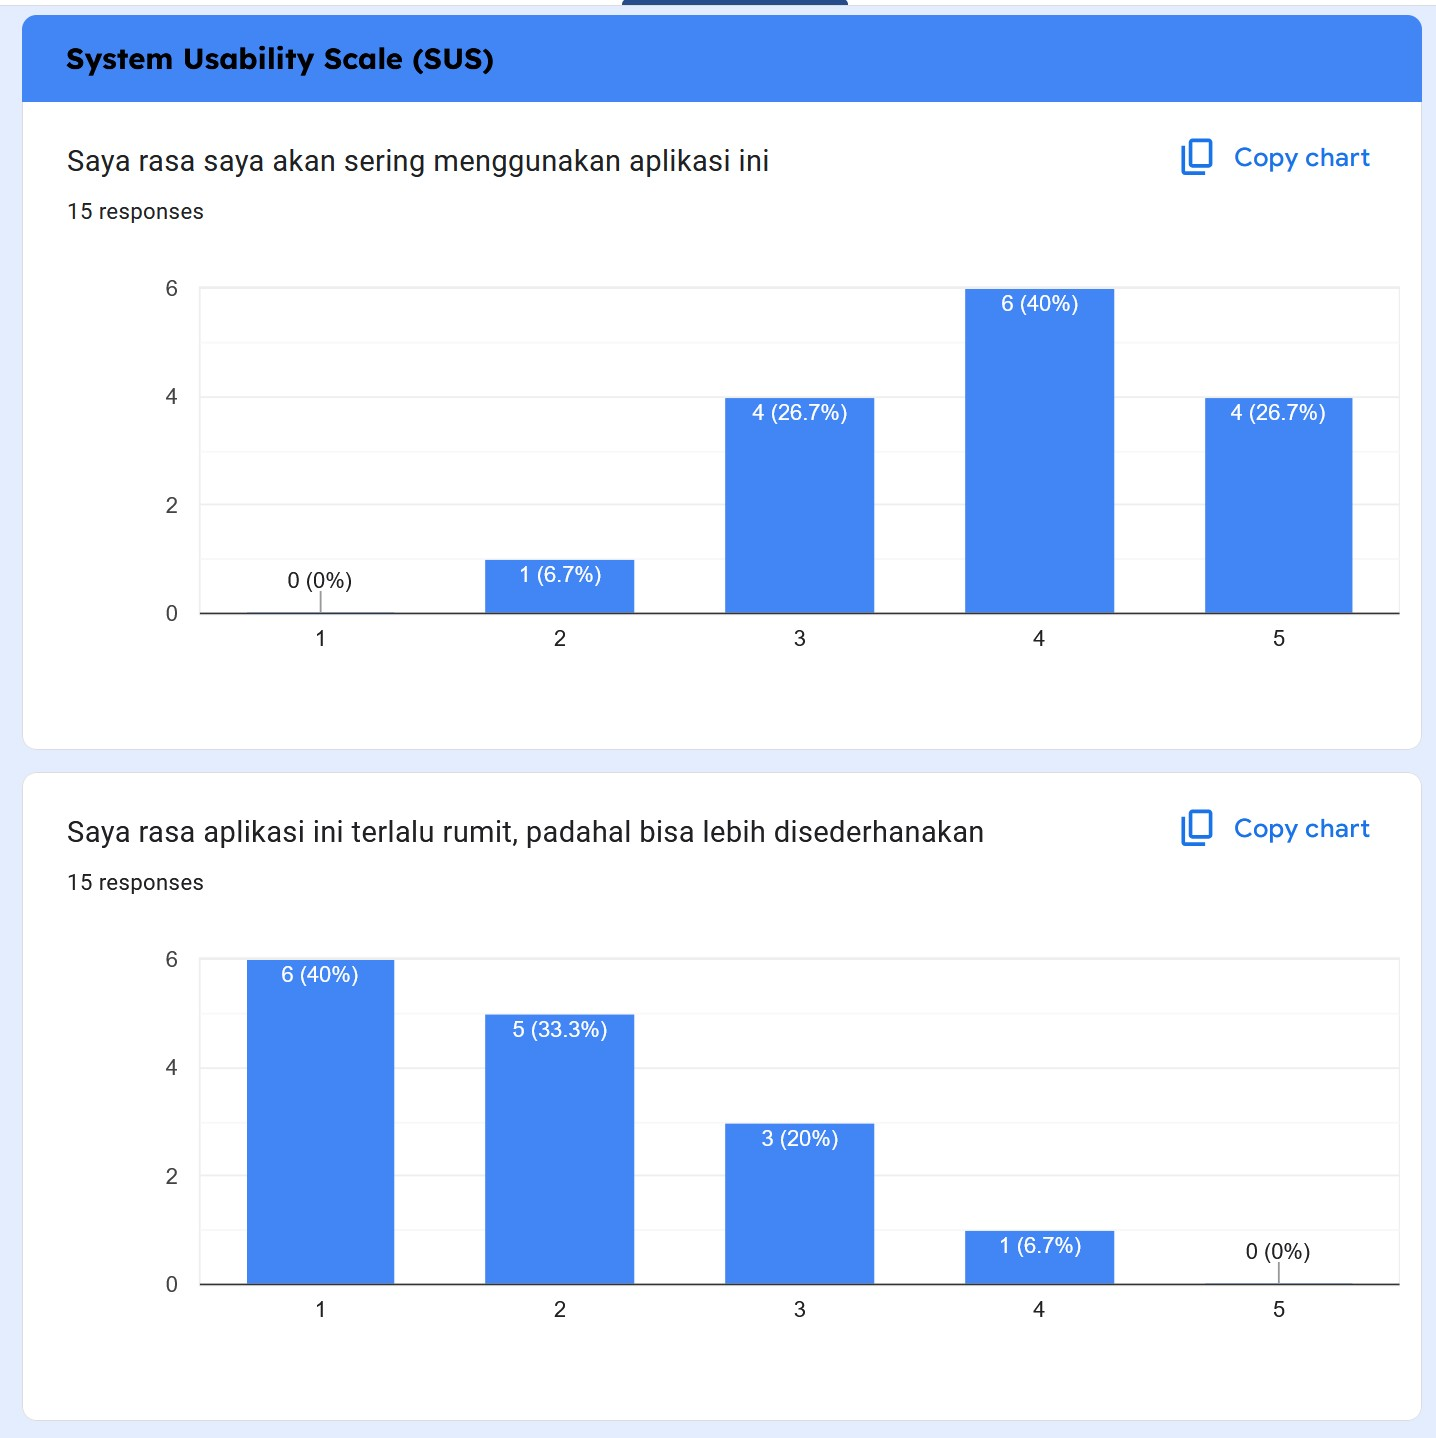
\includegraphics[width=.85\textwidth]{images/eval-pengguna/sus-1-2.jpg}
		\\
    	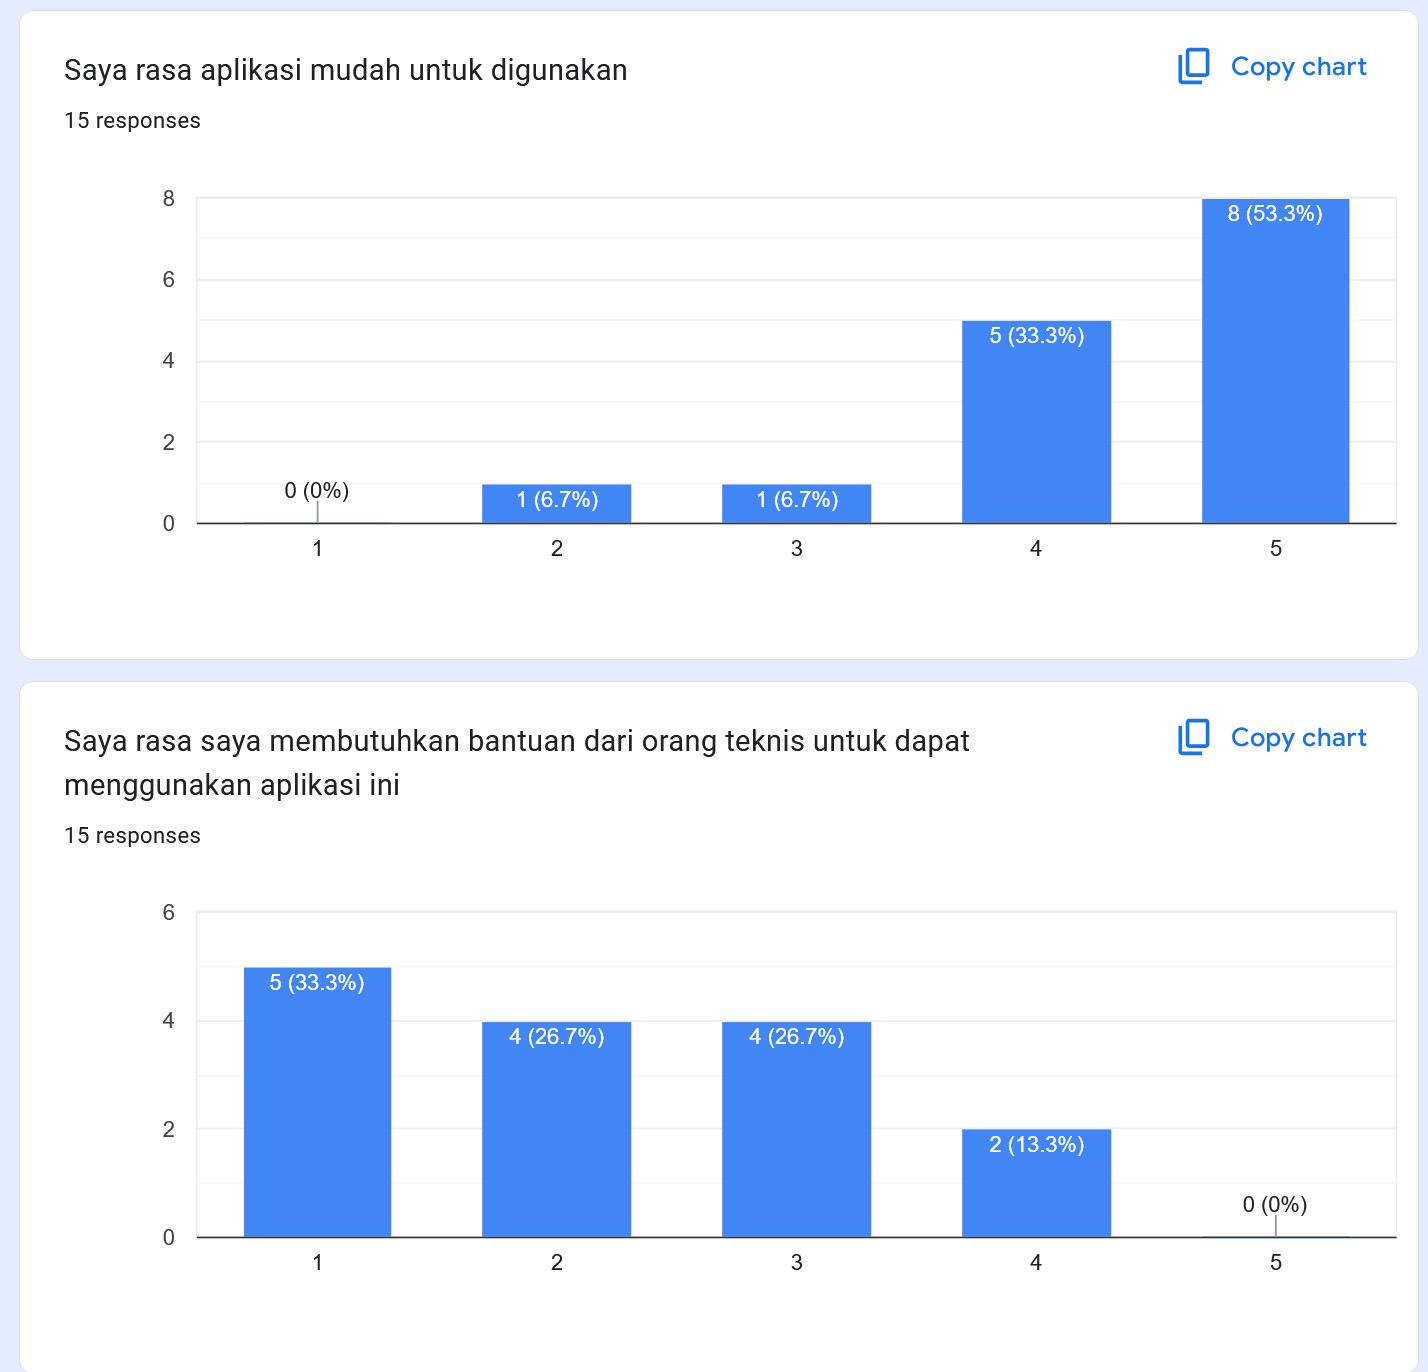
\includegraphics[width=.85\textwidth]{images/eval-pengguna/sus-3-4.jpg}
	\end{minipage}
\end{tabular}

\begin{tabular}{c}
	\begin{minipage}{\linewidth}
		\centering
    	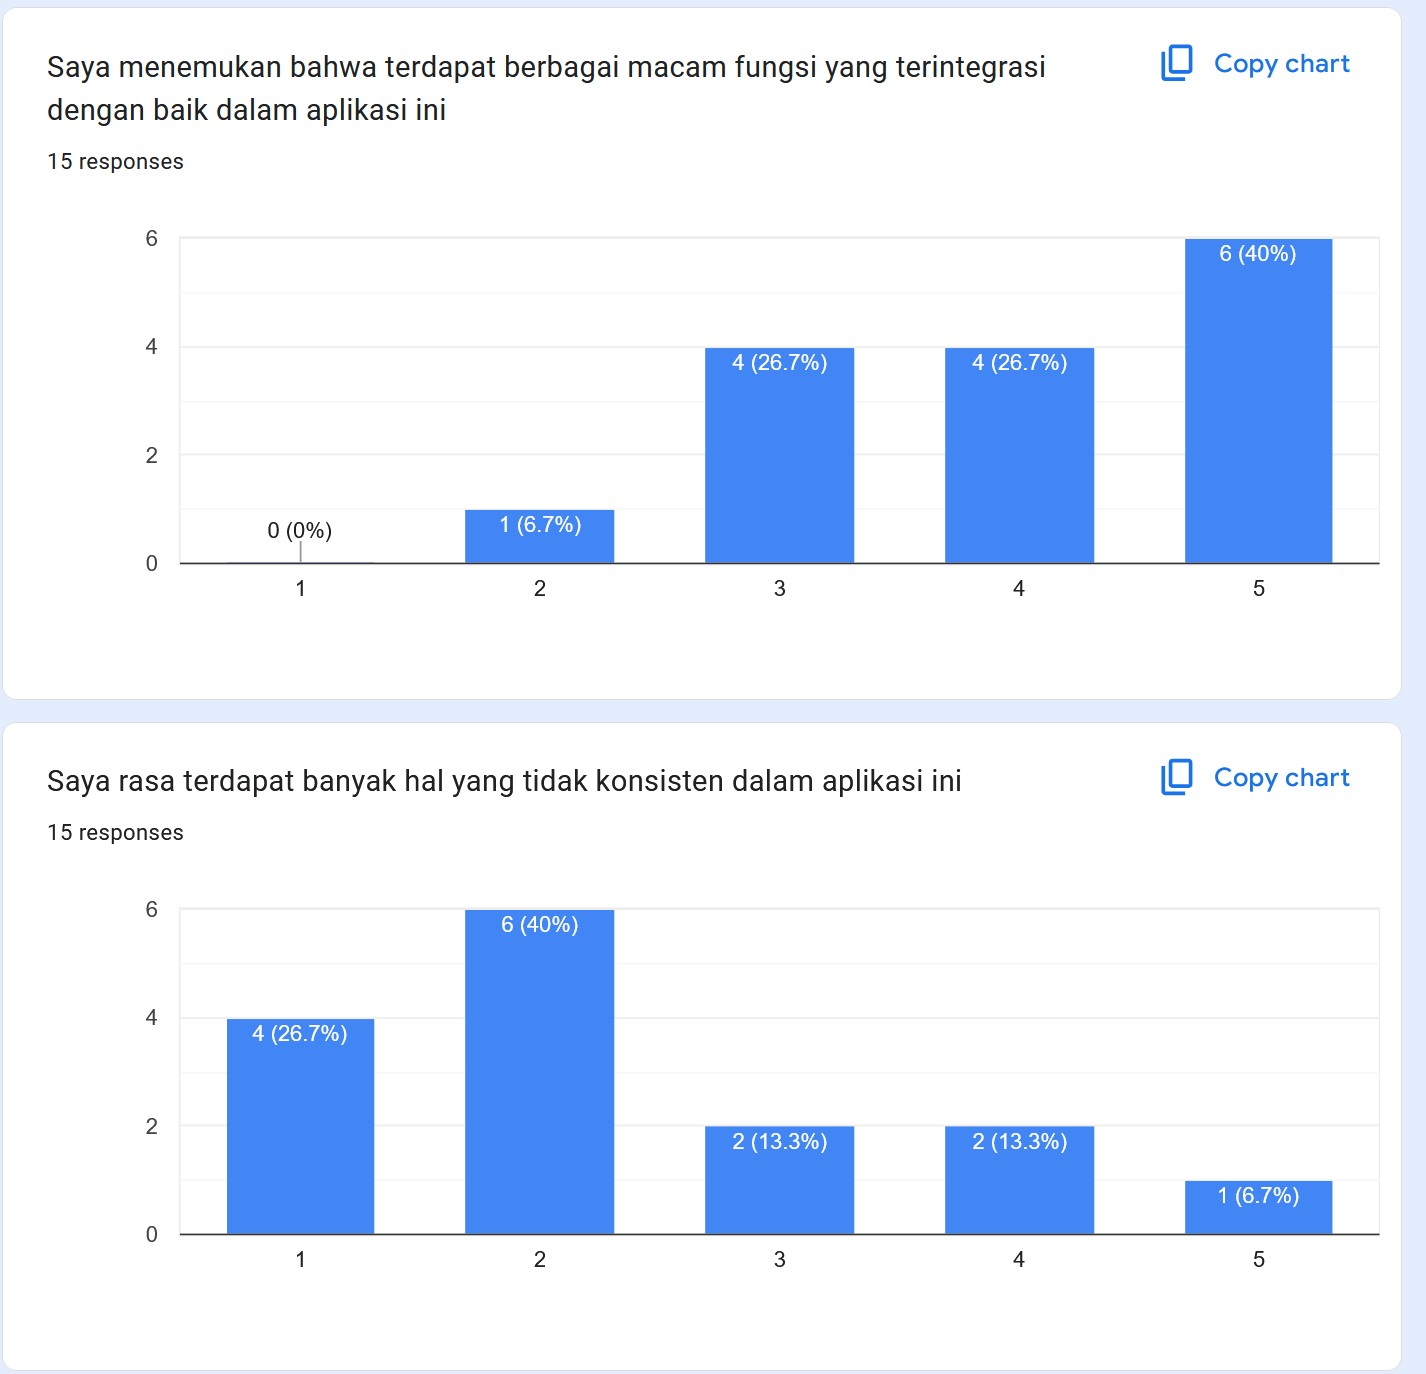
\includegraphics[width=.85\textwidth]{images/eval-pengguna/sus-5-6.jpg} 
		\\
    	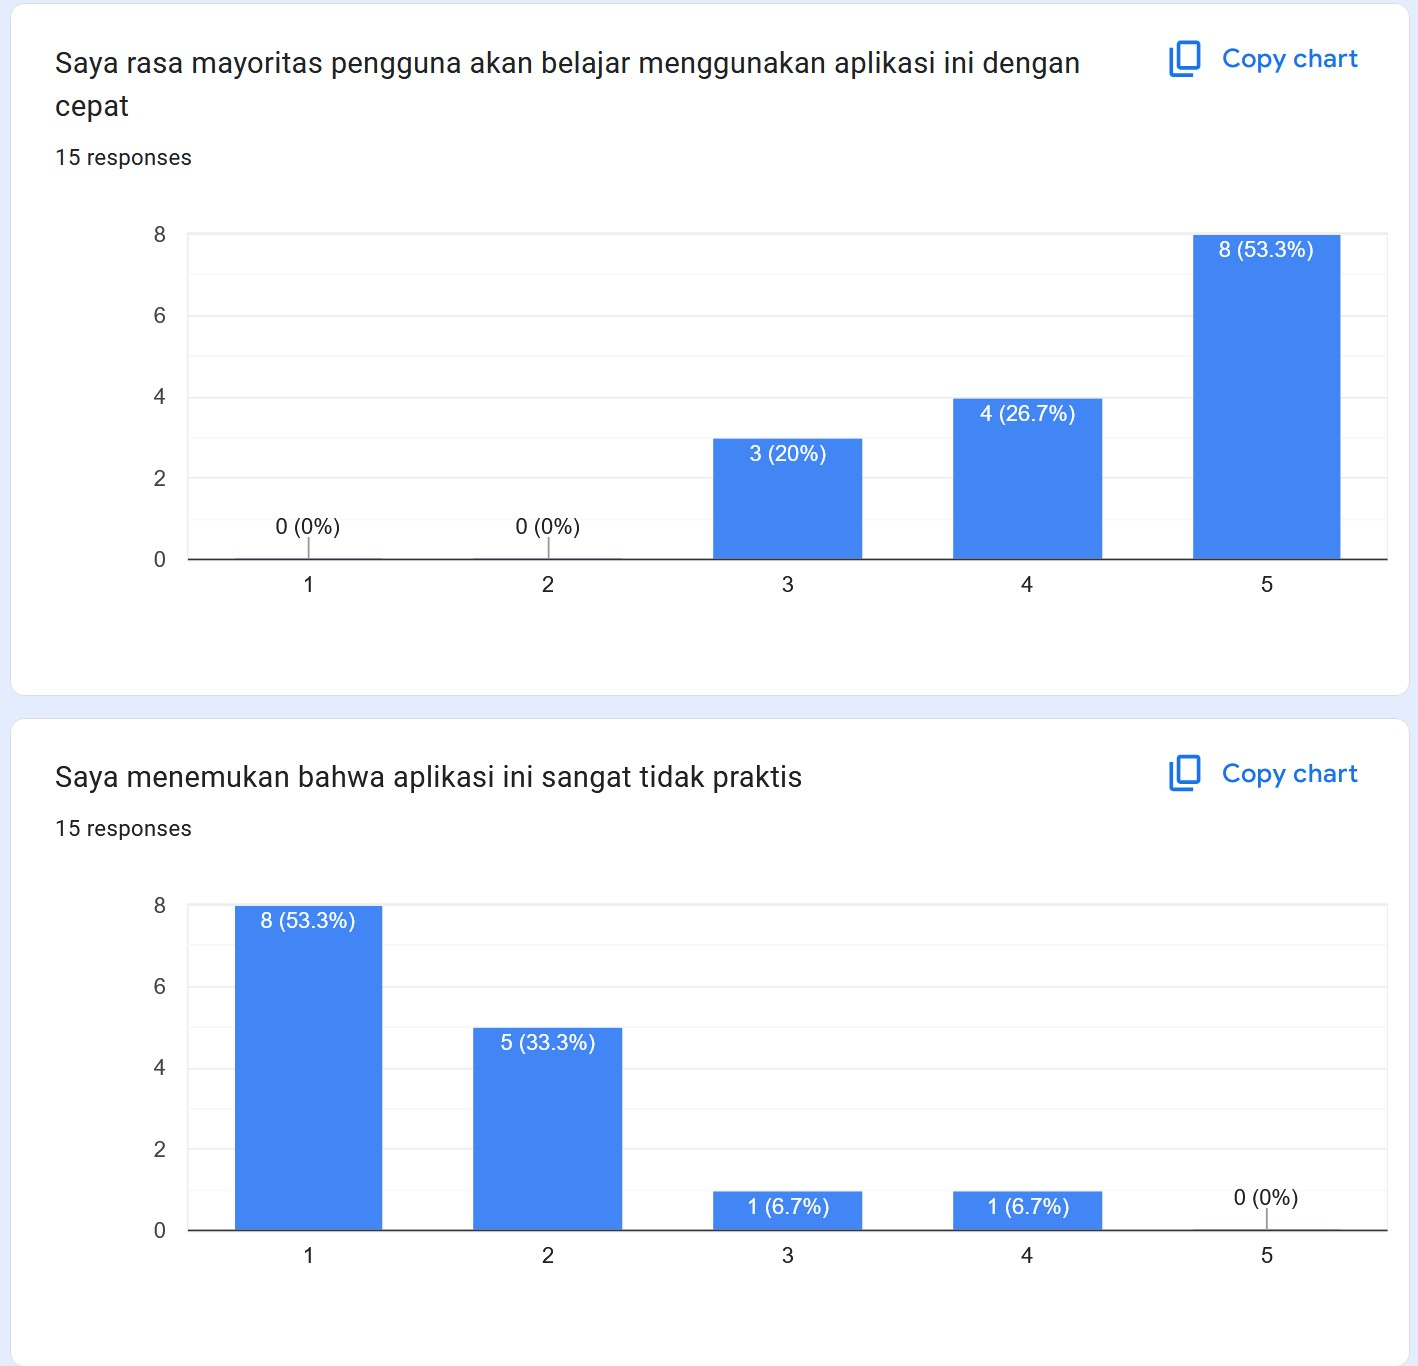
\includegraphics[width=.85\textwidth]{images/eval-pengguna/sus-7-8.jpg}
	\end{minipage}
\end{tabular}

\begin{tabular}{c}
	\begin{minipage}{\linewidth}
		\centering
    	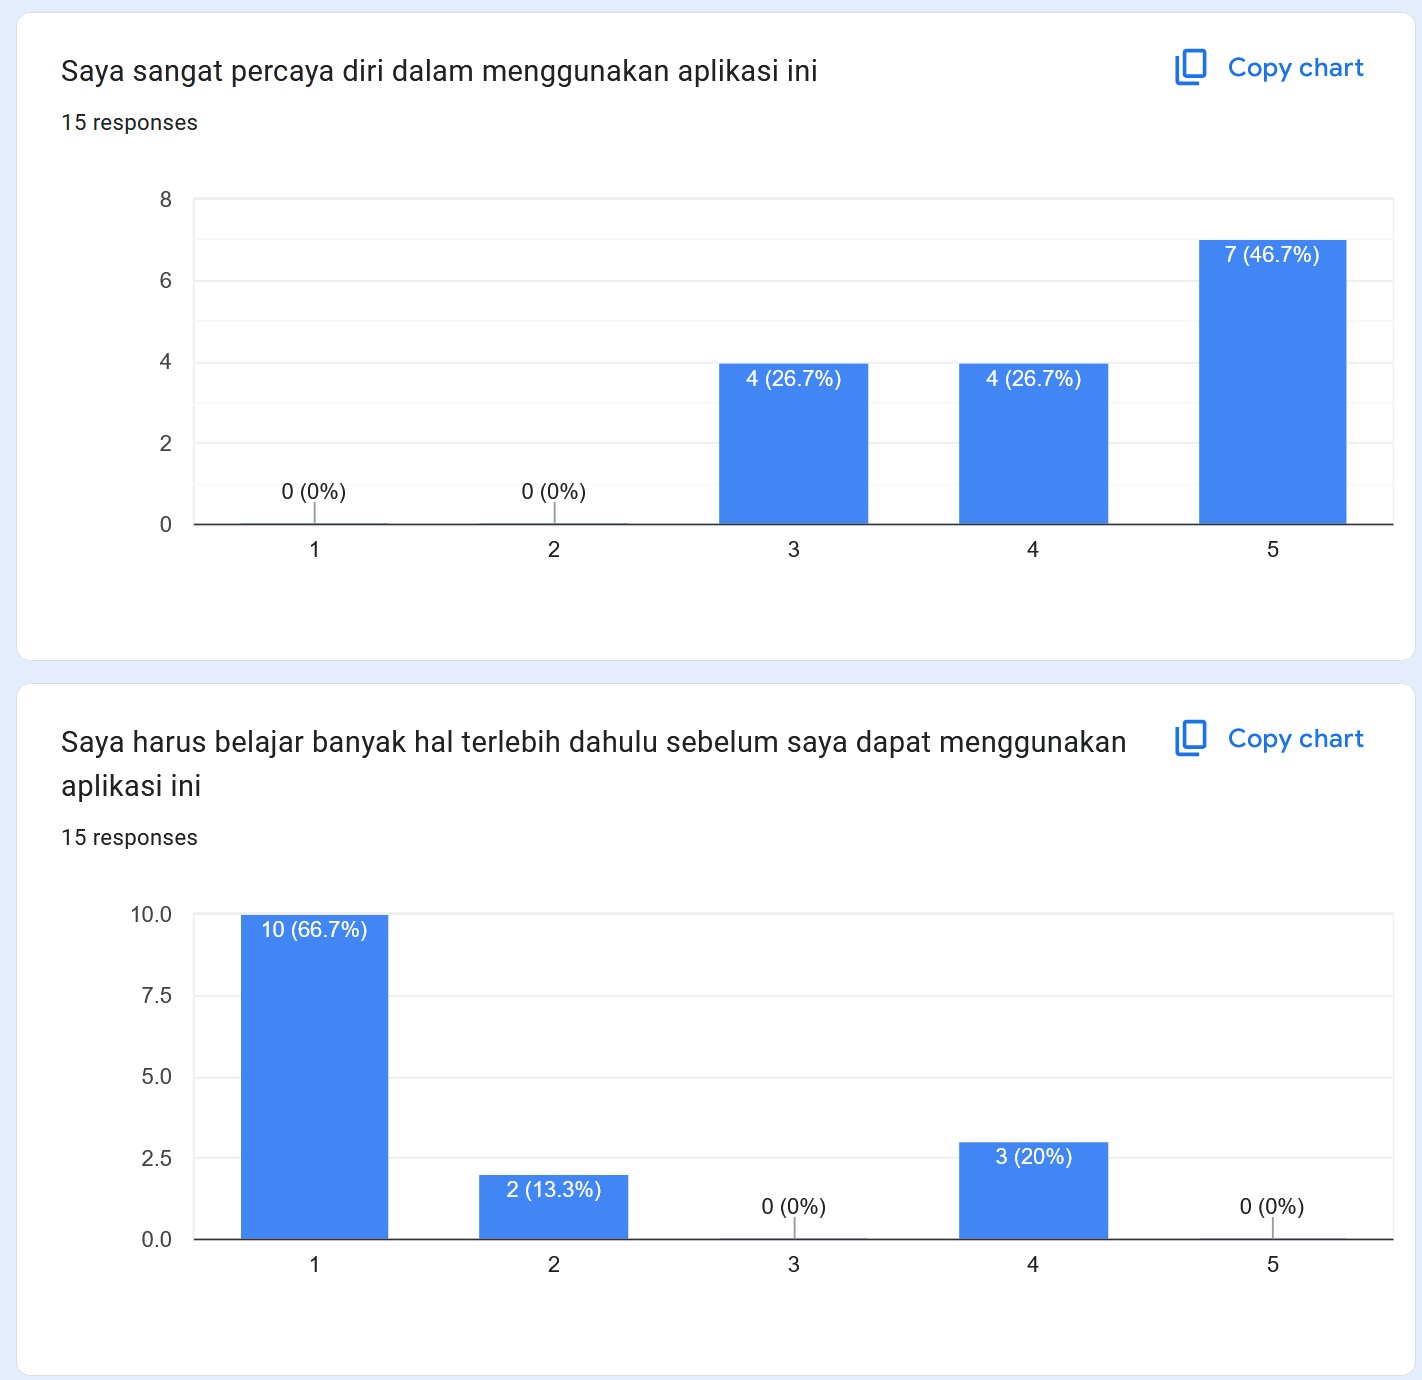
\includegraphics[width=.85\textwidth]{images/eval-pengguna/sus-9-10.jpg} 
		\\
		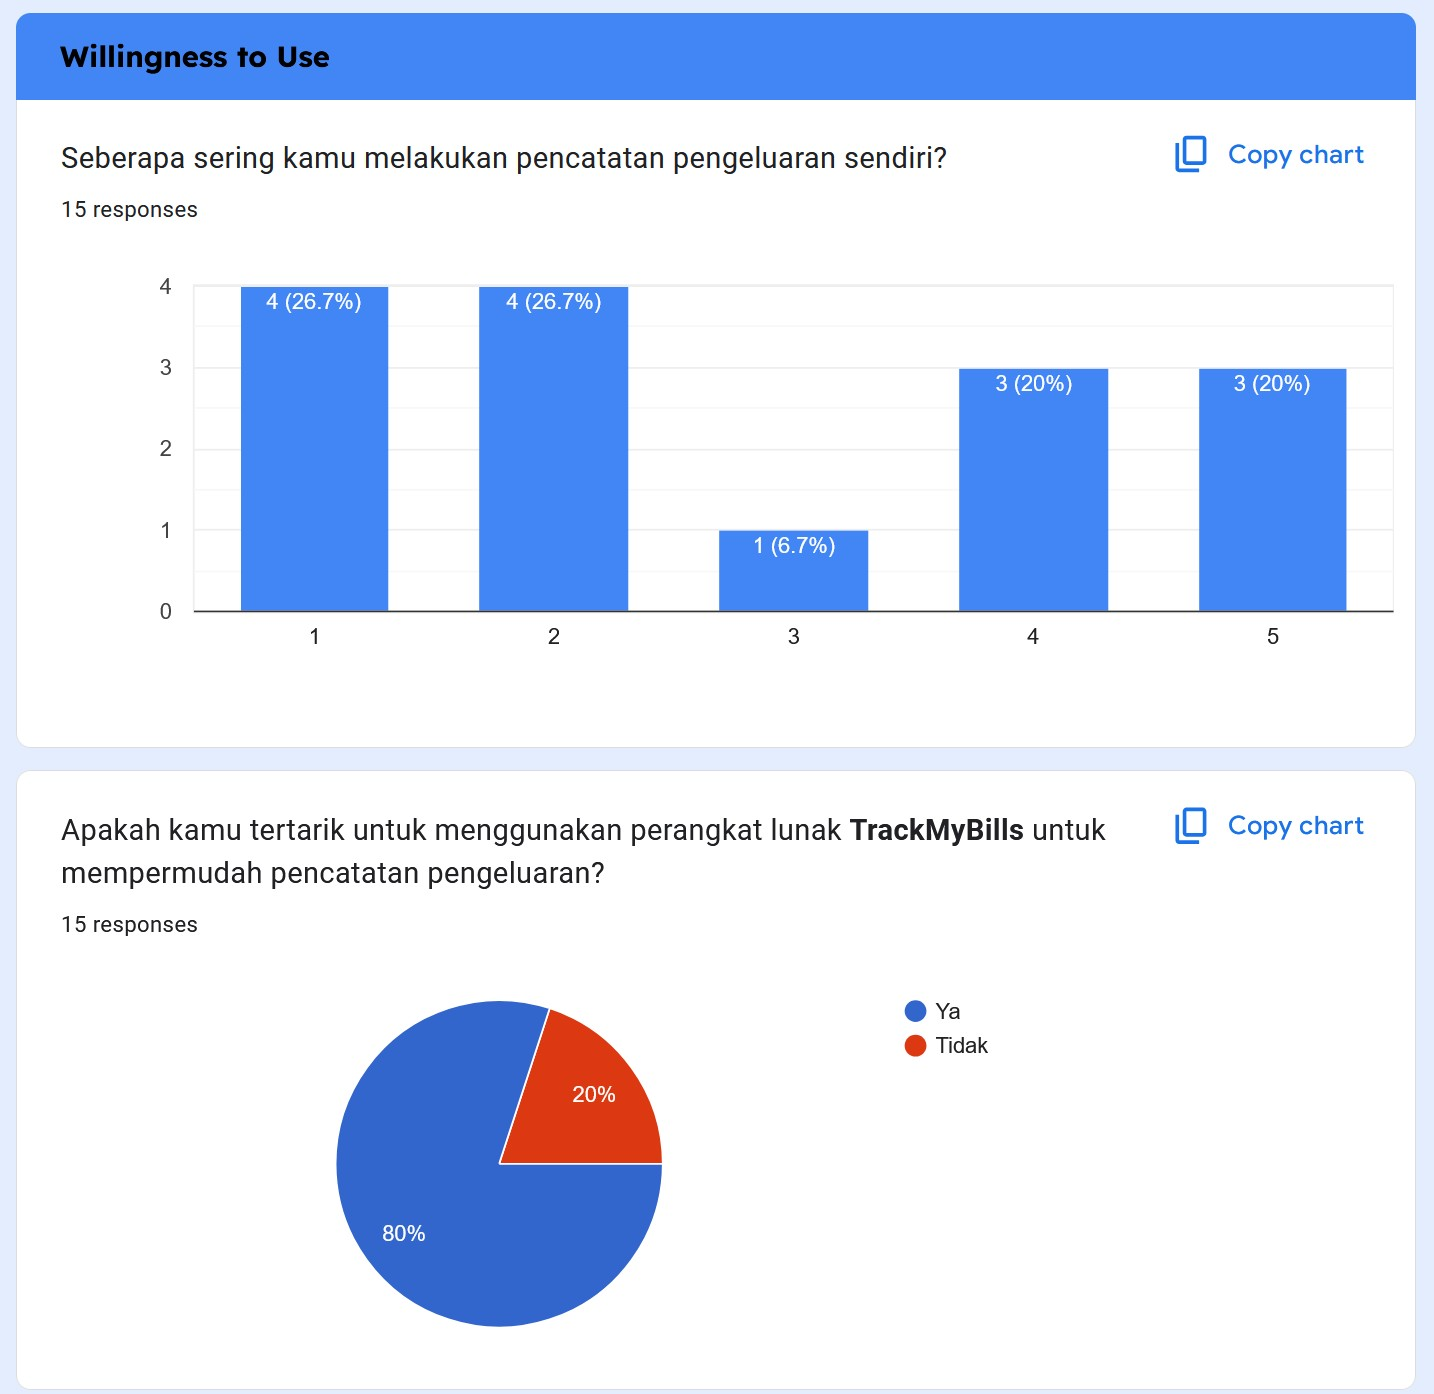
\includegraphics[width=.85\textwidth]{images/eval-pengguna/wil-1.jpg} 
	\end{minipage}
\end{tabular}

\begin{tabular}{c}
	\begin{minipage}{\linewidth}
		\centering
    	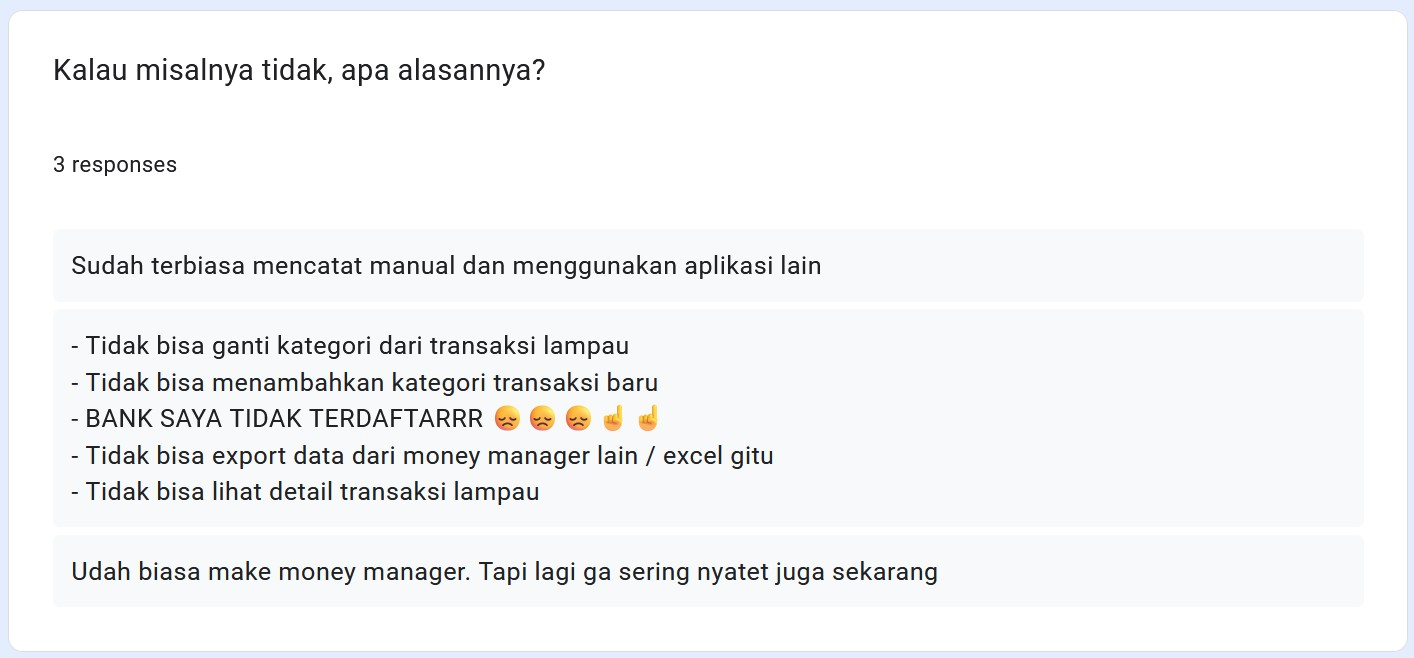
\includegraphics[width=1\textwidth]{images/eval-pengguna/wil-2.jpg} 
		\\
		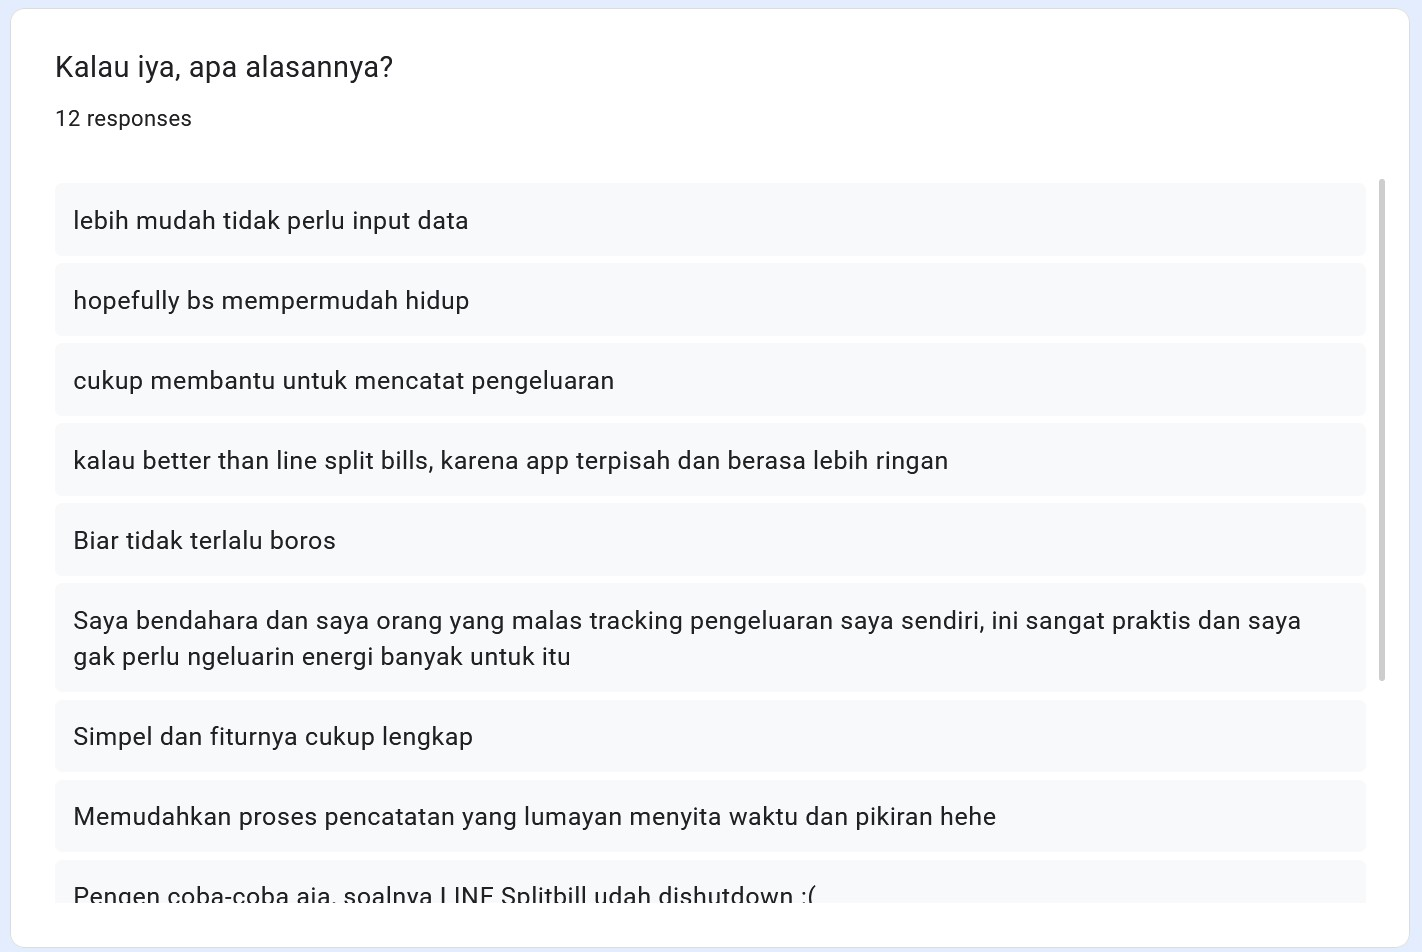
\includegraphics[width=1\textwidth]{images/eval-pengguna/wil-3.jpg} 
		\\
		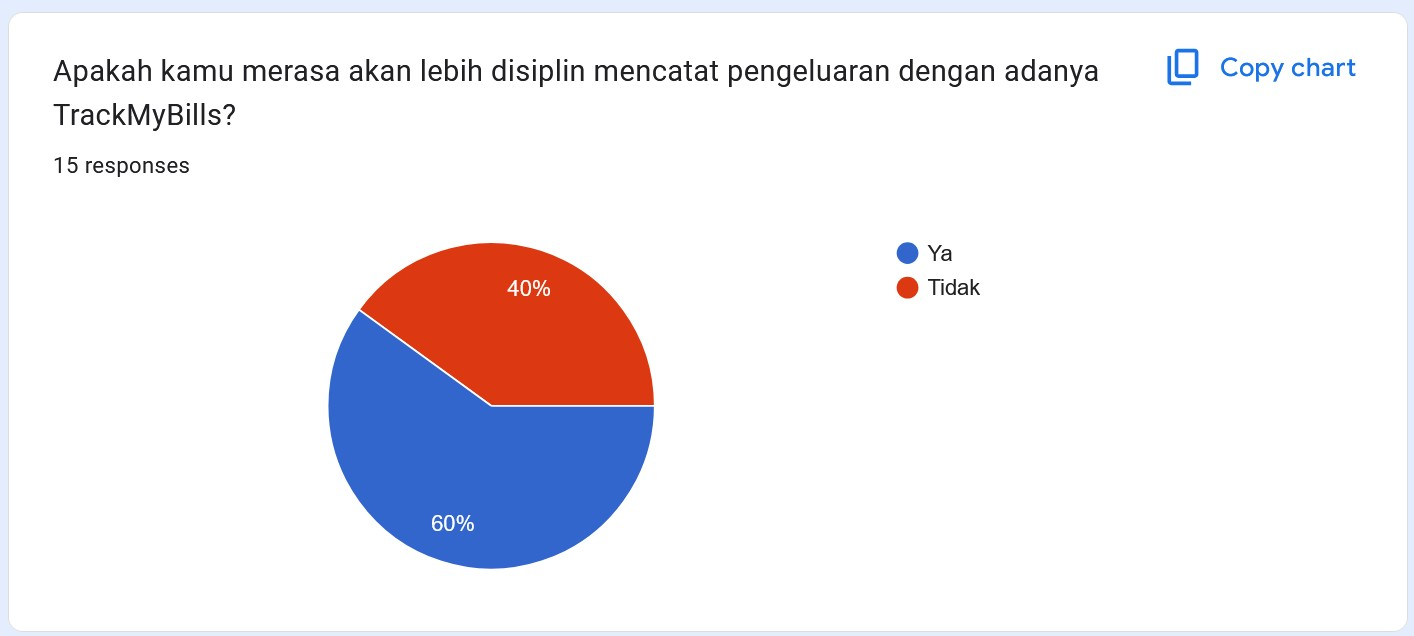
\includegraphics[width=1\textwidth]{images/eval-pengguna/wil-4.jpg}
	\end{minipage}
\end{tabular}

\begin{tabular}{c}
	\begin{minipage}{\linewidth}
		\centering
    	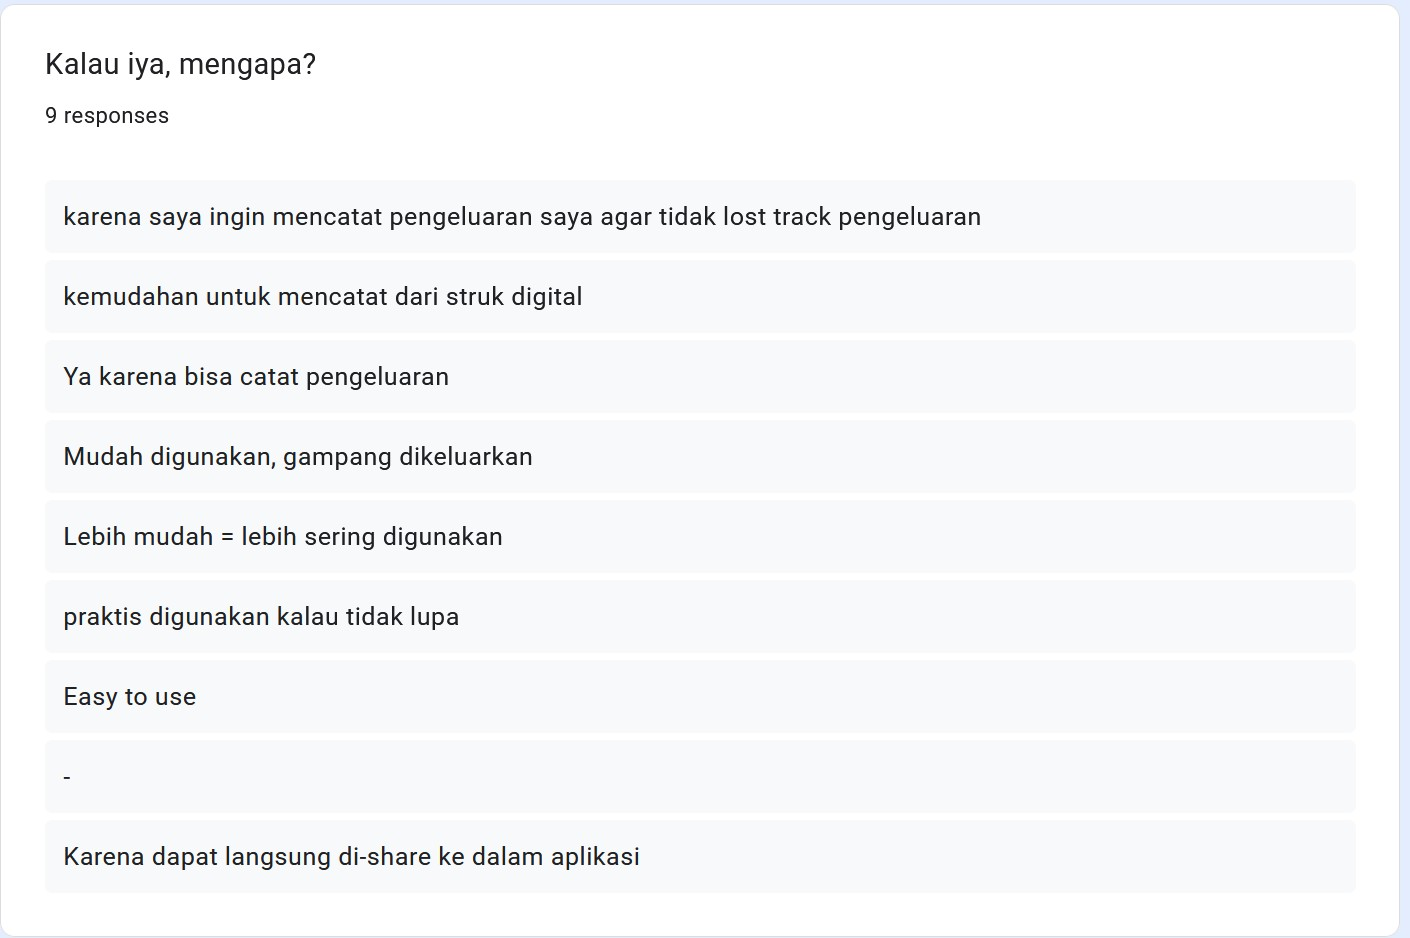
\includegraphics[width=1\textwidth]{images/eval-pengguna/wil-5.jpg} 
		\\
		\includegraphics[width=1\textwidth]{images/eval-pengguna/wil-6.jpg} 
		\\
		\includegraphics[width=1\textwidth]{images/eval-pengguna/wil-7.jpg}
	\end{minipage}
\end{tabular}


\end{document}
